
\documentclass{article}

\PassOptionsToPackage{numbers}{natbib}
\usepackage{neurips_2026}

\usepackage[utf8]{inputenc}
\usepackage[T1]{fontenc}
\usepackage{microtype}
\usepackage{amsmath,amssymb,amsfonts,amsthm,mathtools,bm,mathrsfs}
\usepackage{booktabs}
\usepackage{array}
\usepackage{enumitem}
\usepackage{xcolor}
\usepackage{hyperref}
\usepackage{graphicx}
\usepackage{float}
\usepackage{placeins}
\usepackage{tikz}
\usetikzlibrary{shapes,arrows,arrows.meta,positioning,decorations.markings,decorations.pathmorphing}
\usepackage[compat=1.1.0]{tikz-feynman}

\hypersetup{colorlinks=true,linkcolor=blue!55!black,citecolor=blue!55!black,urlcolor=blue!55!black}

\definecolor{color1}{HTML}{0077BB}
\definecolor{color2}{HTML}{EE7733}
\definecolor{color3}{HTML}{33BBEE}
\definecolor{color4}{HTML}{EE3377}
\definecolor{color5}{HTML}{CC3311}
\definecolor{color6}{HTML}{009988}
\definecolor{color7}{HTML}{BBBBBB}

\pgfdeclaredecoration{parallel}{initial}{%
  \state{initial}[width=0,next state=main]{\pgfpathmoveto{\pgfpointorigin}}%
  \state{main}[width=\pgfdecoratedinputsegmentlength/100]{\pgfpathlineto{\pgfpointorigin}}%
  \state{final}{}%
}

\tikzfeynmanset{
  smallblob/.style={
    /tikz/shape=circle,
    /tikz/draw=black,
    /tikz/fill=white!70!black,
    /tikz/minimum size=6pt,
    /tikz/inner sep=0pt,
    /tikz/graphs/as={}
  },
  quarticblob/.style={
    /tikz/shape=circle,
    /tikz/draw=black,
    /tikz/fill=white!70!black,
    /tikz/minimum size=15pt,
    /tikz/graphs/as={}
  },
  rankblob/.style={
    /tikz/shape=circle,
    /tikz/draw=color2,
    /tikz/fill=color2!18,
    /tikz/minimum size=18pt,
    /tikz/inner sep=1pt,
    /tikz/graphs/as={}
  },
  stiefelblob/.style={
    /tikz/shape=diamond,
    /tikz/draw=color4,
    /tikz/fill=color4!14,
    /tikz/minimum size=17pt,
    /tikz/inner sep=1pt,
    /tikz/graphs/as={}
  },
  projblob/.style={
    /tikz/shape=rectangle,
    /tikz/draw=color5,
    /tikz/fill=color5!10,
    /tikz/minimum size=13pt,
    /tikz/inner sep=1pt,
    /tikz/graphs/as={}
  },
  color1doubghost/.style={
    transform canvas={shift={(0,-1pt)}},
    dash pattern=on 3pt off 3pt,
    line width=1pt,
    draw=color1,
    preaction={
      transform canvas={shift={(0,1pt)}},
      dash pattern=on 3pt off 3pt,
      line width=1pt,
      draw=color1
    }
  },
  color1color2ghost/.style={
    transform canvas={shift={(0,-1pt)}},
    dash pattern=on 3pt off 3pt,
    line width=1pt,
    draw=color2,
    preaction={
      transform canvas={shift={(0,1pt)}},
      dash pattern=on 3pt off 3pt,
      line width=1pt,
      draw=color1
    }
  },
  color6color1ddntknew/.style={
    dash pattern=on 1pt off 1pt,
    line width=1pt,
    draw=color6,
    opacity=0,
    postaction={
      draw=color1,
      opacity=1,
      decorate,
      decoration={parallel,raise=-0.75pt}
    },
    postaction={
      draw=color6,
      opacity=1,
      decorate,
      decoration={parallel,raise=0.75pt}
    }
  }
}

\newtheorem{theorem}{Theorem}[section]
\newtheorem{proposition}[theorem]{Proposition}
\newtheorem{lemma}[theorem]{Lemma}
\newtheorem{corollary}[theorem]{Corollary}
\newtheorem{assumption}[theorem]{Assumption}
\newtheorem{definition}[theorem]{Definition}
\newtheorem{remark}[theorem]{Remark}

\newcommand{\E}{\mathbb E}
\newcommand{\Pp}{\mathbb P}
\newcommand{\R}{\mathbb R}
\newcommand{\cN}{\mathcal N}
\newcommand{\cF}{\mathcal F}
\newcommand{\cX}{\mathcal X}
\newcommand{\Cov}{\operatorname{Cov}}
\newcommand{\Var}{\operatorname{Var}}
\newcommand{\cumul}{\operatorname{cum}}
\newcommand{\tr}{\operatorname{tr}}
\newcommand{\diag}{\operatorname{diag}}
\newcommand{\rank}{\operatorname{rank}}
\newcommand{\relu}{\operatorname{ReLU}}
\newcommand{\op}{\mathrm{op}}
\newcommand{\eps}{\varepsilon}
\newcommand{\gam}{\gamma}
\newcommand{\wh}{\widehat}
\newcommand{\wt}{\widetilde}
\newcommand{\barE}{\bar\varepsilon}
\newcommand{\one}{\mathbf 1}
\newcommand{\NNGP}{\mathrm{NNGP}}
\newcommand{\NTK}{\mathrm{NTK}}
\newcommand{\MLP}{\mathrm{MLP}}
\newcommand{\RF}{\mathrm{RF}}
\newcommand{\LR}{\mathrm{LR}}
\newcommand{\dd}{\mathrm d}
\newcommand{\norm}[1]{\left\lVert #1\right\rVert}

\title{Low-Rank Neural Networks and Finite-Width NTK\\
at the Edge of Convexity}

\author{Anonymous Authors}

\begin{document}
\maketitle

\begin{abstract}
Low-rank neural networks are usually sold as smaller, compressed and pruned models. This paper asks a sharper question: when does low rank still preserve the optimization geometry that makes wide networks trainable? We answer this through the finite-width neural tangent kernel. Low-rank NTK training still carries an interpretable bottleneck-feature geometry, because rank controls which feature maps enter the tangent kernel. Our main result is that low-rank training is governed by a genuine three-way compromise between width, depth, and rank. To the best of our knowledge, this is the first NTK analysis showing that an optimization certificate can impose a depth-rank tradeoff of this form. In particular, for low-rank bottleneck dynamics, preserving the NTK spectral margin has a proven conservative cubic-depth sufficient rule, \(r \gtrsim L^{3}\), up to dataset-size and logarithmic factors. From the finite-network experiments, we conjecture an effective \(L^{3/2}\) law for scalar-output contracted cumulants. We also give a full-rank-compatible parametrization, separating true low-rank effects from ordinary finite-width effects. True finite-network NTK experiments confirm the exact full-rank matching, the predicted operator scaling, the rank-depth tradeoff, and the finite-network cumulant growth. The result is a criterion for when low-rank networks remain trainable for structural reasons, not merely parameter-efficient ones.
\end{abstract}

\section{Introduction}
Low-rank neural networks are usually motivated by efficiency: fewer parameters, lower memory traffic, and cheaper adaptation. This motivation is incomplete. Rank also changes the geometry of training. Low-rank bottlenecks do not merely shrink a dense model: they restrict the network to a small set of bottleneck feature maps, so feature selection already enters through the architecture. Thus saying that an NTK analysis has ``no features'' is misleading for low-rank networks; the question is whether the fixed or linearized low-rank feature geometry remains stable enough to explain training. In the NTK regime, gradient descent is close to kernel regression when the empirical NTK Gram matrix is positive and stable. Thus a low-rank network is useful not only when it is small, but when its finite NTK stays close enough to a positive limiting kernel. We call this the edge of convexity: the regime where the network is finite and structured, but the NTK Gram matrix still provides a convex local training geometry.

Empirically, low-rank bottlenecks can give a much better parameter-accuracy tradeoff than dense baselines. This raises the next theoretical question at very small rank: if only \(r\) bottleneck feature maps are available, which features are recovered, and is the recovery explained by a kernel/NTK mechanism or by genuine feature-learning dynamics such as mean-field or \(\mu\)P scaling? The present paper answers the controlled NTK side of that question. It shows that even in the nominally lazy regime, low-rank bottlenecks introduce nontrivial rank-channel geometry, memory suppression, and spectral constraints that any feature-learning theory must build on.

\begin{table}[t]
\centering
\caption{MNIST parameter-efficiency snapshot. Low-rank bottlenecks recover most of the dense baseline accuracy with far fewer trainable parameters.}
\label{tab:intro-mnist-lowrank}
\begin{tabular}{lrr}
\toprule
Model & Trainable parameters & Test accuracy (\%) \\
\midrule
Dense MLP & 669,706 & 98.39 \\
Low-rank, \(r=5\) & 7,695 & 93.72 \\
Low-rank, \(r=10\) & 10,260 & 96.24 \\
Low-rank, \(r=15\) & 12,825 & 96.97 \\
Low-rank, \(r=25\) & 17,955 & 97.00 \\
Low-rank, \(r=50\) & 30,780 & 97.01 \\
Low-rank trainable factors, \(r=32\) & 440,362 & 98.30 \\
\bottomrule
\end{tabular}
\end{table}

This question is difficult because three limits interact. Width controls ordinary finite-width fluctuations, depth amplifies NTK tensor corrections, and rank changes the channel contractions themselves. Treating low rank as merely replacing \(1/n\) by \(1/r\) misses the full-rank endpoint: if a rank-\(n\) factorization is just an orthogonal change of variables, the low-rank correction must vanish exactly. Conversely, bottleneck random-feature low-rank networks do not reduce to dense MLPs and can suppress old NTK paths geometrically. A useful theory must separate these two cases.

We study random-feature low-rank (RF-LR) scalar-output ReLU networks with layer weights of the form
\begin{equation}
W^{(\ell)}=\frac{\sigma_w}{\sqrt{n_{\ell-1}}}\sqrt{\frac{n_\ell}{r_\ell}}\,U^{(\ell)}B^{(\ell)},
\qquad (U^{(\ell)})^\top U^{(\ell)}=I_{r_\ell},
\label{eq:intro-model}
\end{equation}
where \(U^{(\ell)}\) is frozen and sampled uniformly from the Stiefel manifold
\(\mathrm{St}(n_\ell,r_\ell)=\{U\in\R^{n_\ell\times r_\ell}:U^\top U=I_{r_\ell}\}\), while \(B^{(\ell)}\) is trainable. Thus the Stiefel object is the left factor \(U^{(\ell)}\) itself: its columns form an orthonormal \(r_\ell\)-frame in \(\R^{n_\ell}\), chosen uniformly among all such frames. Equivalently, \(U^{(\ell)}\) selects a random \(r_\ell\)-dimensional subspace with no preferred direction. When \(r_\ell=n_\ell\), the map \(B^{(\ell)}\mapsto U^{(\ell)}B^{(\ell)}\) is an orthogonal reparametrization of a dense MLP. Thus the full-rank endpoint is exact, not asymptotic; Section \ref{sec:stiefel-projector-vertices} identifies the corresponding rank-defect scale.

\section{Related Work}
The NTK formalizes lazy infinite-width training as kernel regression \citep{Jacot2018,Lee2019}. Lee et al. clarified that wide networks of any depth evolve approximately as linear models around initialization, making the empirical NTK spectrum the relevant stability object \citep{Lee2019}. Many global-convergence results rely on keeping this empirical NTK close to a positive limiting kernel \citep{Du2019,AllenZhu2019,Arora2019}. Spectral refinements show that strong guarantees can hold even when only part of a deep network is very wide \citep{NguyenMondelli2020,NguyenMondelliMontufar2022}; recent EOC analyses further study concentration and spectra of MLP NTKs at the edge of chaos \citep{TerjekGonzalezSanchez2025Concentration,TerjekGonzalezSanchez2025Spectrum}. These works provide the dense full-rank baseline; they do not identify the finite-rank correction created by factorized layers or the cancellation that occurs at the full-rank endpoint.

A complementary line studies how finite networks depart from their infinite-width limits. Yang's Tensor Programs give a general language for infinite-width limits, parametrization choices, and feature-learning scalings across architectures \citep{Yang2019,Yang2021,Yang2022MuP,YangDepthMuP2024}, while the neural tangent hierarchy describes finite-width departures from frozen-kernel dynamics \citep{Huang2020}. Feynman-diagram methods organize these corrections by connected cumulants and tensor contractions \citep{DyerGurAri2019,FeynmanNTK2025}. Our analysis follows this perturbative viewpoint, but changes the stochastic source: dense channel contractions are replaced by Stiefel-projector and rank-channel cumulants.

NTK theory is also not meant to replace feature-learning theories. Mean-field limits describe distributional feature evolution beyond the fixed-kernel regime \citep{MeiMontanariNguyen2018,ChizatBach2018,RotskoffVandenEijnden2018}, and \(\mu\)P, depth-\(\mu\)P, tensor-program, and DMFT analyses identify scalings where features continue to move at infinite width \citep{Yang2022MuP,YangDepthMuP2024,BordelonPehlevan2022}. Our results are complementary: they quantify the finite-rank and finite-width stability of the lazy/proxy geometry before one studies full feature-learning dynamics.

Low-rank adaptation and low-rank training have also been analyzed in NTK-like settings, including guarantees that sufficiently large low-rank adapters avoid bad local minima in certain regimes \citep{JangLeeRyu2024LoRA}. Empirical NTK tools make direct finite-network checks feasible \citep{Novak2022}, and recent quantitative GP approximation during training gives another complementary control problem \citep{MosigGarciaAgazziTrevisan2025}. In contrast, our object is the operator deviation of a deep low-rank empirical NTK and the resulting Weyl spectral-preservation criterion.

\paragraph{Contributions.}
First, full-rank factorization is only a coordinate change: when \(r=n\), the empirical NTK matches the dense MLP pathwise. Away from full rank, the correction is a projector defect, not the naive replacement \(n\mapsto r\).

The second message is that depth turns small rank defects into a stability constraint. Low-rank randomness enters locally at each layer, but NTK legs are transported through the whole network. One transported leg creates a larger accumulated correction than a pure NNGP fluctuation, and two transported NTK legs create the worst depth growth. This is the mechanism behind the conservative cubic rank-depth rule for bottleneck dynamics: deep low-rank networks are hard to keep in the same convex NTK regime unless rank grows with depth.

The third message is practical. The theory gives an operator-level stability certificate under an explicit well-spread data assumption, and it remains closed under the NTK descendants that control short-time training drift. The experiments then check the pieces separately: exact full-rank matching, disappearance of the rank defect at \(r=n\), the predicted depth normalization, and direct finite-network cumulants. The observed slopes are effective exponents of mixed observable quantities, so they also point to a sharper future theory beyond the worst-case cubic envelope.

\section{Models and Full-Rank Matching}
This section defines the factorized network, proves exact matching at full rank, and explains why the left factor is frozen.

For a fixed dataset \(x_1,\ldots,x_m\), the scalar-output empirical NTK is
\begin{equation}
\wh\Theta_{ab}=\nabla_\theta f(x_a)\cdot \nabla_\theta f(x_b).
\end{equation}
In \eqref{eq:intro-model}, the trainable parameters are the right factors \(B^{(\ell)}\) and the readout. We keep \(U^{(\ell)}\) frozen so the tangent space is a fixed subspace and all rank-dependent randomness enters through \(G=(n/r)UU^\top\). Training \(U\) would move the subspace and add \(U\)-\(B\) dNTK interaction terms.

\begin{theorem}[Pathwise full-rank matching]
\label{thm:pathwise}
If \(r_\ell=n_\ell\) for every hidden layer, then for every realization, dataset, and depth, the empirical NTK in \(B\)-coordinates equals the dense MLP NTK in coordinates \(\wt W^{(\ell)}=U^{(\ell)}B^{(\ell)}\). The same equality holds for the NNGP, dNTK, ddNTK, and their tensor cumulants.
\end{theorem}

\begin{proof}
When \(r=n\), \(U\) is orthogonal, so \(\Delta B\mapsto U\Delta B\) preserves Frobenius inner products. Hence \(J_BJ_B^\top=J_WJ_W^\top\), and higher derivatives and cumulants are invariant under the same coordinate change.
\end{proof}

\begin{proposition}[Why the left factor is frozen]
\label{prop:frozen-left}
For one layer \(W=\alpha UB\), with \(U^\top U=I_r\) and \(H=\partial \mathcal L/\partial W\), training only \(B\) gives
\begin{equation}
\nabla_B\mathcal L=\alpha U^\top H,
\qquad
\dot W_B=-\eta\alpha^2UU^\top H.
\label{eq:frozen-left-flow}
\end{equation}
If \(U\) is also trained on the Stiefel manifold, the normal projected component contributes
\begin{equation}
\dot W_U
=-\eta\alpha^2 (I-UU^\top)H B^\top B
\quad
\text{up to rotations inside } \operatorname{span}(U)\text{ that can be absorbed into }B.
\label{eq:moving-left-flow}
\end{equation}
Thus moving \(U\) adds \(U\)-\(B\) interaction blocks proportional to \(B^\top B\), absent from the frozen-left model and not controlled solely by cumulants of \(G=(n/r)UU^\top\).
\end{proposition}

\begin{proof}[Proof idea]
Project the Euclidean gradient onto the \(B\)-directions and the Stiefel tangent space, then map both variations back to \(W=\alpha UB\); this gives \eqref{eq:frozen-left-flow} and \eqref{eq:moving-left-flow}. The full differential calculation is in Appendix \ref{app:frozen-left-full-proof}.
\end{proof}

Freezing \(U\) therefore isolates the rank-width effect and keeps the diagrammatics closed under the Stiefel projector vertices of Lemma \ref{lem:stiefel-cov}.

The RF-LR bottleneck has a different recursion,
\begin{equation}
\Theta^{(\ell)}=1+\frac1r\Theta^{(\ell-1)}\dot\Sigma^{(\ell)}+\frac1r\Sigma^{(\ell)}.
\label{eq:rflr-recursion}
\end{equation}
Here we suppress the sample pair \((x,x')\). If \((g_x^{(\ell)},g_{x'}^{(\ell)})\) is the Gaussian preactivation pair induced by the previous-layer covariance, then
\begin{equation}
\Sigma^{(\ell)}(x,x')
:=\E\!\left[\sigma(g_x^{(\ell)})\sigma(g_{x'}^{(\ell)})\right],
\qquad
\dot\Sigma^{(\ell)}(x,x')
:=\E\!\left[\sigma'(g_x^{(\ell)})\sigma'(g_{x'}^{(\ell)})\right].
\label{eq:rflr-sigma-definitions}
\end{equation}
Thus \(\Sigma^{(\ell)}\) is the NNGP covariance term injected at layer \(\ell\), while \(\dot\Sigma^{(\ell)}\) is the derivative covariance multiplying an old NTK line. At the ReLU fixed point \(\dot\Sigma^{(\ell)}\to1/2\), so an old NTK contribution is multiplied by approximately \((2r)^{-(L-k)}\). This is a different model, not a perturbation of the dense MLP.

\section{Stiefel Projector Vertices}
\label{sec:stiefel-projector-vertices}
This section explains the random projector \(G=(n/r)UU^\top\), which is the only way the frozen random left factor enters the NTK corrections.
Let \(U\in\R^{n\times r}\) be sampled uniformly from the Stiefel manifold and
\begin{equation}
G=\frac nr UU^\top.
\label{eq:projector-G}
\end{equation}
We study this Stiefel projector because the trainable gradients with respect to \(B\) are always projected through the random subspace selected by \(U\); therefore cumulants of \(G\) are the low-rank replacement for dense neuron-index contractions. Orthogonal invariance gives the full covariance tensor.

\begin{lemma}[Stiefel projector covariance]
\label{lem:stiefel-cov}
For all indices,
\begin{equation}
\begin{aligned}
\Cov(G_{ij},G_{kl})
&=\gamma_{n,r}\left(\delta_{ik}\delta_{jl}+\delta_{il}\delta_{jk}
-\frac2n\delta_{ij}\delta_{kl}\right),\\
\gamma_{n,r}
&=\frac{n(n-r)}{r(n-1)(n+2)}
=\frac1r-\frac1n+O(n^{-2}).
\end{aligned}
\label{eq:stiefel-cov}
\end{equation}
In particular \(\gamma_{n,n}=0\). The mixed perturbation parameter is therefore \(1/n+\gamma_{n,r}\): the \(1/n\) term is the ordinary dense finite-width correction, while \(\gamma_{n,r}\) is the rank defect. The rank-defect part vanishes at \(r=n\), exactly as required by pathwise full-rank matching.
\end{lemma}

\begin{proof}
The covariance of a Stiefel projector has the invariant form \(a(\delta_{ik}\delta_{jl}+\delta_{il}\delta_{jk})+b\delta_{ij}\delta_{kl}\). The identity \(\tr G=n\) gives \(2a+nb=0\). The standard second moment of a Stiefel projector gives \(a=\gamma_{n,r}\), hence \eqref{eq:stiefel-cov}.
\end{proof}

Higher cumulants are given by orthogonal Weingarten contractions. Connected \(s\)-point cumulants scale as \(O_s(r^{1-s})\) and vanish in the full-rank endpoint. Thus the low-rank Feynman rule is simple: dense Gaussian-ReLU vertices remain, and each low-rank correction inserts connected cumulants of \(G\).

\iffalse
\begin{lemma}[Rank cumulant power counting]
\label{lem:rank-cumulant-counting}
Fix a layer \(\ell\) and condition on all previous layers. For rank channel \(a\), let
\[
Z_a^{(\ell)}
:=
\left\{
\bigl(g_a^{(\ell)}(x_u),\sigma(g_a^{(\ell)}(x_u)),\sigma'(g_a^{(\ell)}(x_u))\bigr)_{u=1}^{m},
\text{ and the corresponding derivative atoms}
\right\}.
\]
Here \(g_a^{(\ell)}(x_u)\) is the scalar preactivation of rank channel \(a\) on sample \(x_u\), after the deterministic conditioning on layer \(\ell-1\). Thus \(Z_a^{(\ell)}\) is the full local random object from which one-channel quantities such as \(\sigma\sigma\), \(\sigma\sigma'\), \(\sigma'\sigma'\), and derivative insertions are evaluated. The variables \(Z_1^{(\ell)},\ldots,Z_r^{(\ell)}\) are conditionally iid. To simplify notation, write them as \(Z_a\), and assume the local functions below have uniformly bounded moments of all orders. Define empirical observables
\[
X_i^{(r)}=r^{-a_i}\sum_{a=1}^{r} f_i(Z_a),
\qquad i=1,\ldots,s.
\]
Then the connected cumulant satisfies
\begin{equation}
\cumul\left(X_1^{(r)},\ldots,X_s^{(r)}\right)
=r^{1-\sum_i a_i}\,
\cumul\left(f_1(Z),\ldots,f_s(Z)\right).
\label{eq:rank-cumulant-counting}
\end{equation}
In particular, normalized empirical averages have \(s\)-point cumulants of order \(r^{1-s}\).
\end{lemma}

\begin{proof}
By multilinearity of cumulants,
\[
\cumul(X_1^{(r)},\ldots,X_s^{(r)})
=r^{-\sum_i a_i}
\sum_{a_1,\ldots,a_s=1}^{r}
\cumul(f_1(Z_{a_1}),\ldots,f_s(Z_{a_s})).
\]
The key point is the conditional independence introduced by the rank-channel representation. If the indices \(a_1,\ldots,a_s\) split across two or more distinct rank channels, then the corresponding random variables can be partitioned into independent groups; by the connectedness property of cumulants, that term is zero. Thus independence kills every cross-channel contribution and leaves only the fully connected one-channel terms \(a_1=\cdots=a_s\). There are exactly \(r\) such terms, all identical, giving \eqref{eq:rank-cumulant-counting}. This cancellation is the heart of the low-rank bookkeeping: after conditioning on the previous layer, the analysis reduces to one-channel cumulants multiplied by the explicit power of \(r\), rather than to a large collection of interacting channel contractions.
\end{proof}

This elementary lemma is the right-factor-only analogue of the usual width power counting. It explains why finite-rank bias terms are typically \(O(r^{-1})\) after averaging over seeds, while single-seed fluctuations are \(O_{\Pp}(r^{-1/2})\). It also explains why the exact full-rank endpoint must be treated with the projector defect \(G-I\), rather than by the informal replacement \(n\mapsto r\).
\fi

The rank-channel power counting is the usual connected-cumulant counting for iid empirical averages: a connected \(s\)-point rank vertex scales as \(r^{1-s}\). Lemma \ref{lem:rank-cumulant-counting} in Appendix \ref{app:rank-power-counting} gives the precise statement and defines the channel atom \(Z_a^{(\ell)}\). This is why finite-rank bias terms are typically \(O(r^{-1})\), while the full-rank endpoint must be treated through the projector defect \(G-I\), not by the informal replacement \(n\mapsto r\).

\begin{figure}[t]
\centering
\begin{minipage}{0.30\linewidth}
\centering
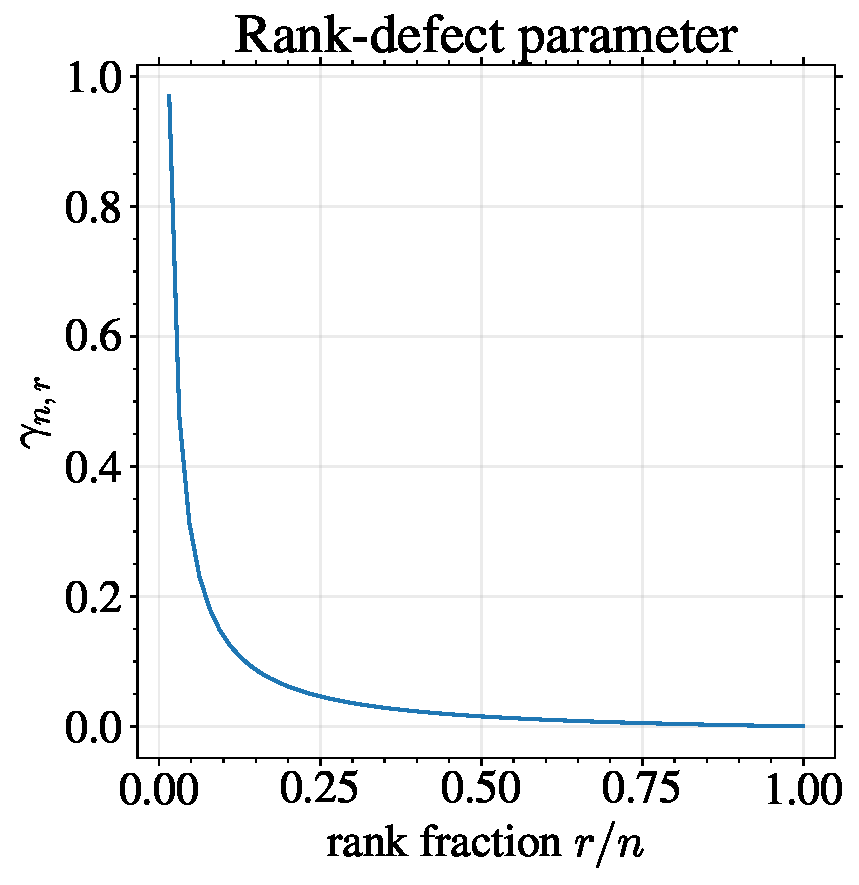
\includegraphics[width=0.92\linewidth]{../../data/feynman/lowrank_ntk_proxy_outputs_clean/rank_defect_gamma.pdf}
\end{minipage}
\hfill
\begin{minipage}{0.30\linewidth}
\centering
\begin{tikzpicture}
\node[anchor=south west,inner sep=0pt] (img) at (0,0)
{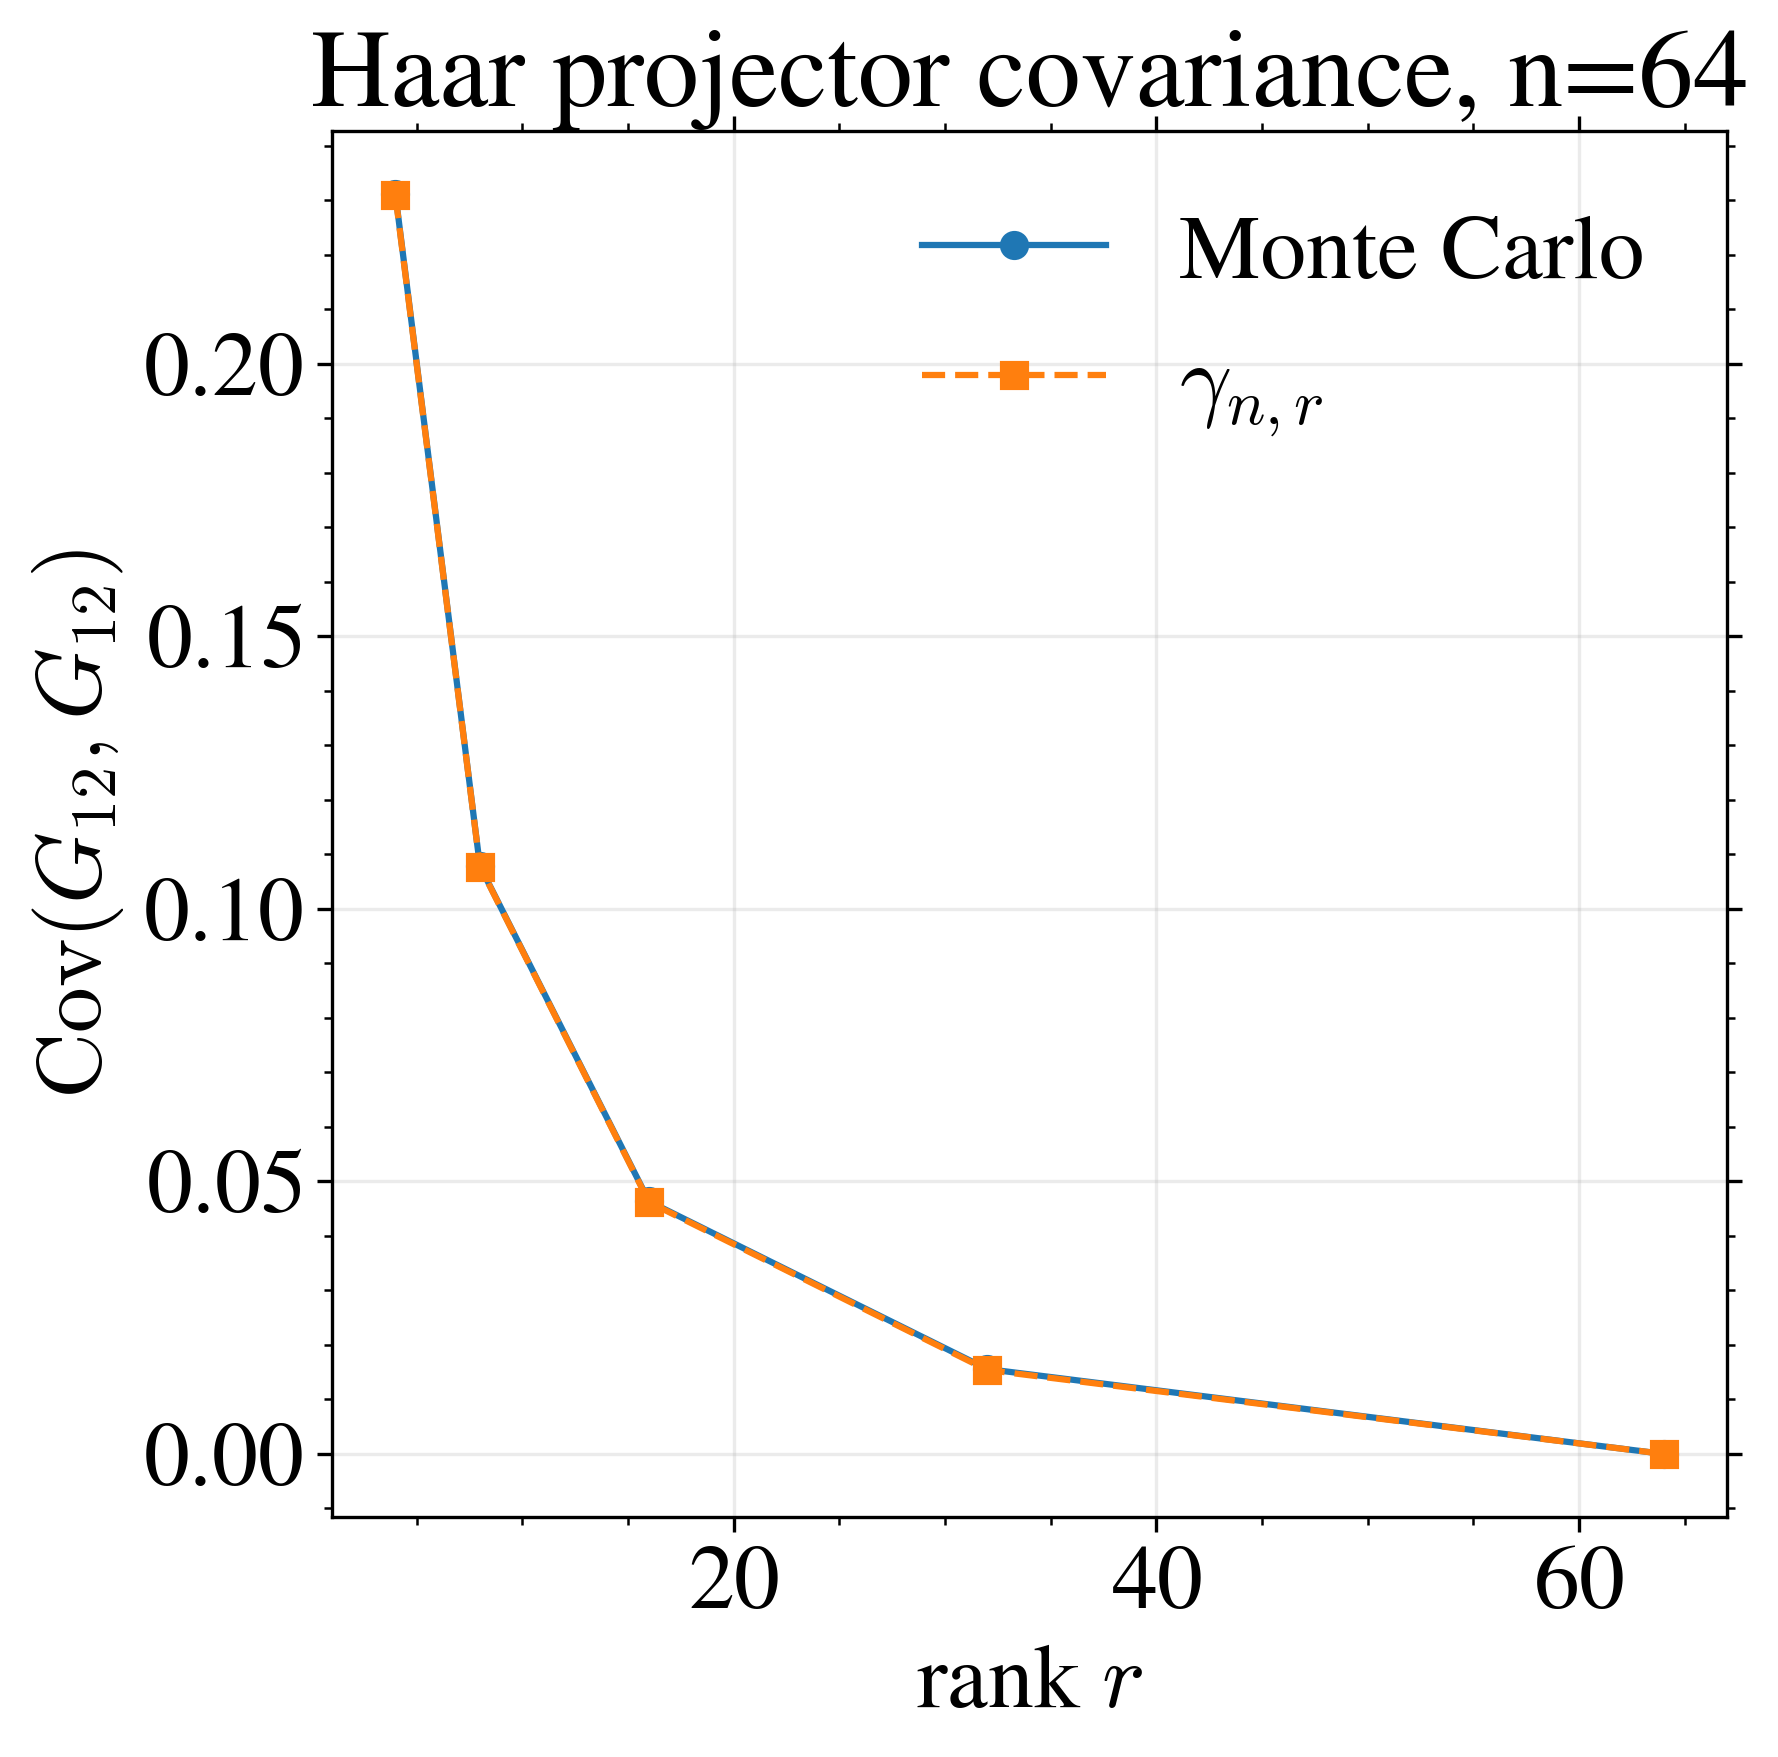
\includegraphics[width=0.92\linewidth]{../../data/feynman/lowrank_ntk_proxy_outputs_clean/stiefel_covariance.png}};
\begin{scope}[x={(img.south east)},y={(img.north west)}]
\fill[white] (0.08,0.88) rectangle (0.92,1.0);
\node[font=\scriptsize] at (0.5,0.945) {Stiefel projector covariance, \(n=64\)};
\end{scope}
\end{tikzpicture}
\end{minipage}
\hfill
\begin{minipage}{0.30\linewidth}
\centering
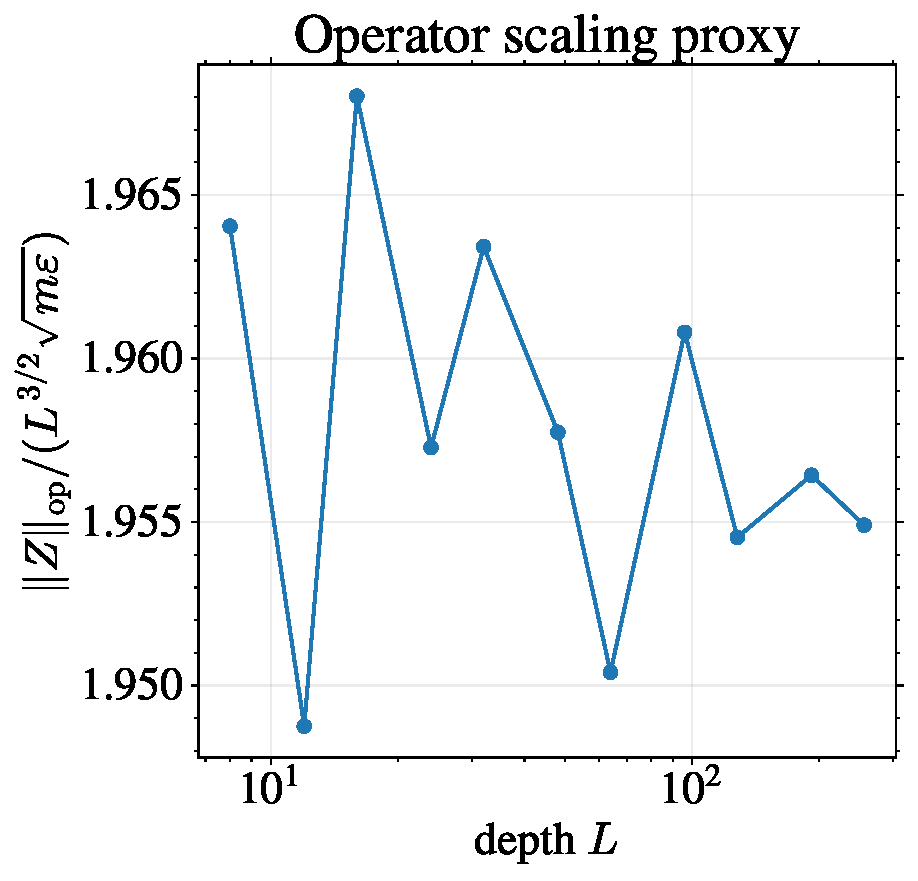
\includegraphics[width=0.92\linewidth]{../../data/feynman/lowrank_ntk_proxy_outputs_clean/operator_proxy_ratio.pdf}
\end{minipage}
\vspace{-0.5em}
\caption{Rank-projector and operator checks. Left: the rank-defect scale \(\gamma_{n,r}\) vanishes at full rank. Middle: empirical Stiefel-projector covariance matches the closed form. Right: the normalized operator proxy \(\|Z\|_{\op}/(L^{3/2}\sqrt{m\eps})\) is approximately stable across depth.}
\label{fig:proxy-stiefel-operator}
\end{figure}

\vspace{-1.0em}
\subsection{Triangular tensor recursion}
The full pairing-basis dictionary for \(V,D,F,A,B\) is in Appendix \ref{app:full-tensor-dictionary}. In the main text we use the compressed block notation \(\mathcal V=(V_{1234},V_{1324},V_{1423})\), \(\mathcal C=(D_{1234},F_{1324},F_{1423})\), and \(\mathcal A=(A_{1234},B_{1324},B_{1423})\).
\iffalse
\begin{align}
V_{1234}^{(\ell)}
&:=\cumul(\delta K_{12}^{(\ell)},\delta K_{34}^{(\ell)})
=\E[\delta K_{12}^{(\ell)}\delta K_{34}^{(\ell)}],
\nonumber\\
D_{1234}^{(\ell)}
&:=\cumul(\delta K_{12}^{(\ell)},\delta\Theta_{34}^{(\ell)})
=\E[\delta K_{12}^{(\ell)}\delta\Theta_{34}^{(\ell)}],
\nonumber\\
F_{1324}^{(\ell)}
&:=\cumul(\delta K_{13}^{(\ell)},\delta\Theta_{24}^{(\ell)})
=\E[\delta K_{13}^{(\ell)}\delta\Theta_{24}^{(\ell)}],
\nonumber\\
A_{1234}^{(\ell)}
&:=\cumul(\delta\Theta_{12}^{(\ell)},\delta\Theta_{34}^{(\ell)})
=\E[\delta\Theta_{12}^{(\ell)}\delta\Theta_{34}^{(\ell)}],
\nonumber\\
B_{1324}^{(\ell)}
&:=\cumul(\delta\Theta_{13}^{(\ell)},\delta\Theta_{24}^{(\ell)})
=\E[\delta\Theta_{13}^{(\ell)}\delta\Theta_{24}^{(\ell)}].
\label{eq:main-tensor-definitions}
\end{align}
The missing pairing coordinates \(V_{1423}\), \(F_{1423}\), and \(B_{1423}\) are obtained by replacing \((13|24)\) with \((14|23)\). Thus \(V\) is the NNGP-NNGP block, \(D,F\) are the mixed NNGP-NTK sectors, and \(A,B\) are the NTK-NTK sectors.
\fi

The layer recursion is triangular at first perturbative order:
\begin{align}
\mathcal V_{\ell+1}
&=
\mathcal L_V^{(\ell)}\mathcal V_\ell+\mathcal S_V^{(\ell)},\\
\mathcal C_{\ell+1}
&=
\mathcal L_C^{(\ell)}\mathcal C_\ell
+\mathcal B_C^{(\ell)}\mathcal V_\ell
+\mathcal S_C^{(\ell)},\\
\mathcal A_{\ell+1}
&=
\mathcal L_A^{(\ell)}\mathcal A_\ell
+\mathcal B_A^{(\ell)}\mathcal C_\ell
+\mathcal Q_A^{(\ell)}[\mathcal V_\ell,\mathcal V_\ell]
+\mathcal S_A^{(\ell)}.
\label{eq:tensor-triangular-recursion}
\end{align}

\begin{figure}[H]
\centering
\begin{minipage}{0.30\linewidth}
\centering
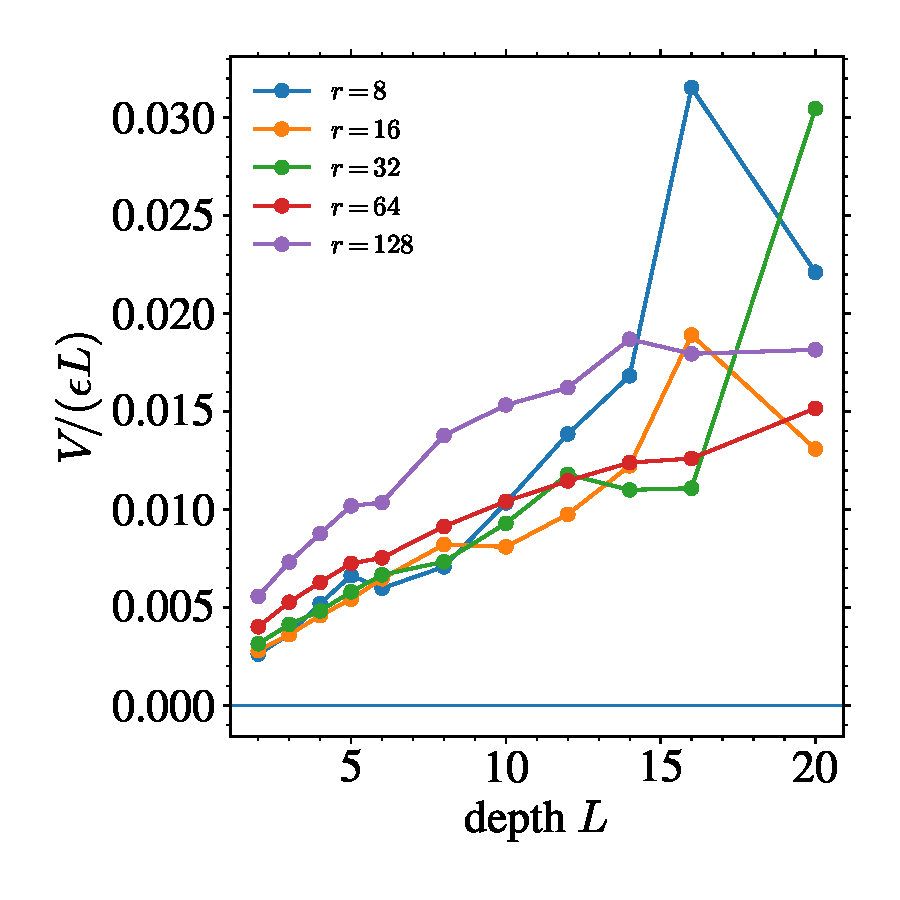
\includegraphics[width=0.92\linewidth]{../../data/feynman/true_finite_ntk_cumulants_very_long/cumulant_ratio_V_same_off_over_eps_L.pdf}
\end{minipage}
\hfill
\begin{minipage}{0.30\linewidth}
\centering
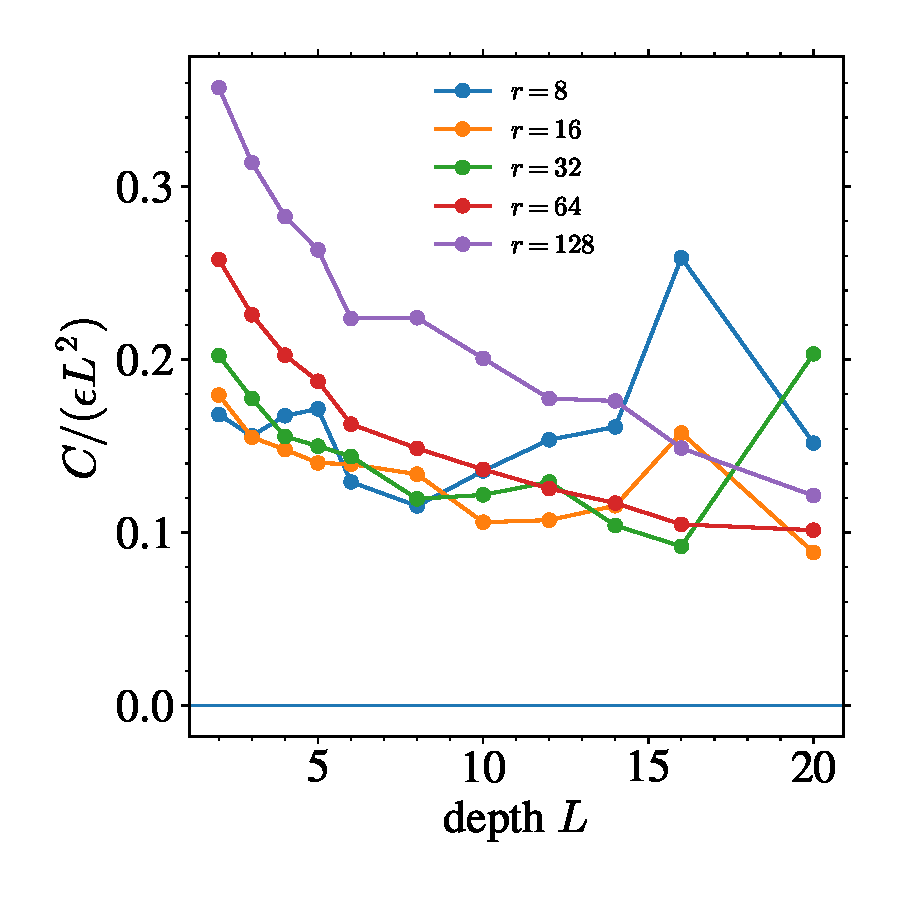
\includegraphics[width=0.92\linewidth]{../../data/feynman/true_finite_ntk_cumulants_very_long/cumulant_ratio_C_same_off_over_eps_L2.pdf}
\end{minipage}
\hfill
\begin{minipage}{0.30\linewidth}
\centering
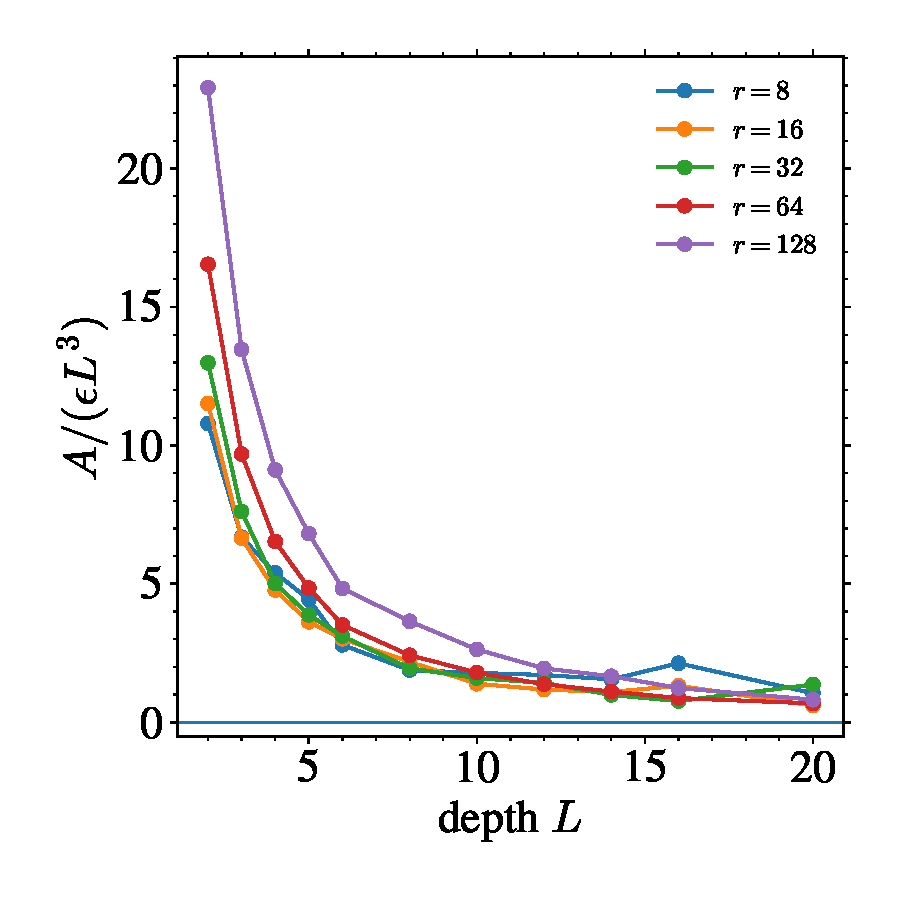
\includegraphics[width=0.92\linewidth]{../../data/feynman/true_finite_ntk_cumulants_very_long/cumulant_ratio_A_same_off_over_eps_L3.pdf}
\end{minipage}
\vspace{-0.5em}
\caption{True finite-network cumulants from autodiff NTKs. These scalar-output cumulants are not isolated Feynman coefficients; they test the predicted polynomial control and rank-width scaling on actual finite networks.}
\label{fig:true-cumulants}
\end{figure}

The source bounds used in Proposition \ref{prop:tensor-hierarchy} are
\begin{equation}
\|\mathcal S_V^{(\ell)}\|\le C,\qquad
\|\mathcal S_C^{(\ell)}\|\le C(1+\ell+\|\mathcal V_\ell\|),\qquad
\|\mathcal S_A^{(\ell)}\|\le C(1+\ell^2+\ell\|\mathcal V_\ell\|+\|\mathcal C_\ell\|+\|\mathcal V_\ell\|^2).
\label{eq:tensor-source-bounds}
\end{equation}
These formulas are the visible mechanism behind the hierarchy: \(V\) feeds \(D,F\), and \(D,F\) feed \(A,B\).

\section{Tensor Scaling at ReLU Edge of Chaos}
This section turns the projector cumulants into depth scalings for the tensor blocks \(V,D,F,A,B\).
For normalized ReLU, the edge-of-chaos correlation asymptotics used in the RF-LR analysis give
\(\theta_\ell=3\pi/\ell+O(\log \ell/\ell^2)\), and
\begin{equation}
\dot{\mathcal C}(\rho_\ell)=1-\frac3\ell+O\left(\frac{\log\ell}{\ell^2}\right).
\label{eq:relu-transport}
\end{equation}
Transporting an external NTK leg from layer \(k\) to \(L\) gives the factor \((k/L)^\lambda\) for an exponent \(\lambda\in\{0,3\}\), depending on whether the Gram entry is diagonal or off-diagonal.

\begin{lemma}[Depth-transport accumulation]
\label{lem:transport-source}
Let \(T_\ell\in\R^d\), \(\ell\ge2\), satisfy \(T_2=0\) and
\begin{equation}
T_{\ell+1}
=\left(I-\frac{M}{\ell}+E_\ell\right)T_\ell+\ell^\beta(s+e_\ell),
\label{eq:transport-source-recursion}
\end{equation}
where \(\norm{E_\ell}\le C\log^p(\ell)/\ell^2\), \(\norm{e_\ell}\le C\log^q(\ell)/\ell\), every eigenvalue of \(M\) has real part greater than \(-(\beta+1)\), and \(M+(\beta+1)I\) is invertible. Then
\begin{equation}
T_L
=L^{\beta+1}\left(M+(\beta+1)I\right)^{-1}s
+O\left(L^\beta\log^{p+q+2}L\right).
\label{eq:transport-source-solution}
\end{equation}
\end{lemma}

\begin{proof}[Proof idea]
Iterating \eqref{eq:transport-source-recursion} gives a variation-of-constants formula; Appendix \ref{app:transport-hierarchy-proof} gives the full discrete proof with the product estimates. The product of propagators from \(k\) to \(L\) is \((k/L)^M\) up to a summable perturbative error. Thus, at leading order,
\[
T_L=L^{-M}\sum_{k\le L} k^{M+\beta I}s+O(L^\beta\log^{p+q+2}L).
\]
Euler-Maclaurin yields
\[
L^{-M}\sum_{k\le L} k^{M+\beta I}
=L^{\beta+1}\int_0^1u^{M+\beta I}\,\dd u+O(L^\beta),
\]
and the matrix integral is \((M+(\beta+1)I)^{-1}\).
\end{proof}

Let \(\barE=\max_{\ell\le L}(1/n_\ell+\gamma_{n_\ell,r_\ell})\). The finite-width tensors obey
\begin{equation}
V_L=O(\barE L),\qquad C_L=O(\barE L^2),\qquad A_L=O(\barE L^3),
\label{eq:main-scales}
\end{equation}
where \(C\) denotes the mixed NNGP-NTK block \((D,F)\), and \(A\) denotes the NTK-NTK block \((A,B)\).

\begin{proposition}[Conditional tensor hierarchy]
\label{prop:tensor-hierarchy}
Assume the low-rank cumulant recursion closes on the same tensor sectors as the dense finite-width Feynman hierarchy and that the ReLU edge-of-chaos transport is uniform away from the diagonal singularity. Then the isolated tensor coordinates satisfy
\begin{equation}
V_L=O(\barE L),\qquad
D_L,F_L=O(\barE L^2),\qquad
A_L,B_L=O(\barE L^3).
\label{eq:tensor-hierarchy}
\end{equation}
Consequently, the perturbative mean-NTK correction is controlled in the regime \(L^3\barE\ll 1\).
\end{proposition}

\begin{proof}[Proof idea]
Appendix \ref{app:transport-hierarchy-proof} gives the complete block-recursion proof. The fresh NNGP four-point source contributes \(O(\barE)\) per layer and has no transported NTK leg in the dominant radial mode, so summation gives \(V_L=O(\barE L)\). The mixed blocks \(D,F\) have one transported NTK leg and therefore one depth-transport accumulation with \(\beta=1\), yielding \(O(\barE L^2)\) by Lemma \ref{lem:transport-source}. The NTK-NTK blocks \(A,B\) have two transported NTK legs, equivalently source exponent \(\beta=2\), giving \(O(\barE L^3)\). These are isolated tensor coordinates; scalar-output cumulants can mix these sectors.
\end{proof}

\paragraph{Endpoint constants.}
At the ReLU endpoint, set \(X_0=2(g_+)^2\) and \(Y_0=2\one_{\{g>0\}}\). Then
\begin{equation}
\Var(X_0)=5,
\qquad
\Cov(X_0,Y_0)=1,
\qquad
\Var(Y_0)=1.
\end{equation}
The table should be read together with the plots. On the standard long run, the visible slopes are indeed close across ranks, with effective exponents around \(1.5\)--\(2.1\) for the same-off-diagonal observables. This supports the interpretation that the proven \(L^3\) tensor bound is a safe upper envelope, not a claim that every scalar-output cumulant must scale exactly as \(L^3\). A natural conjecture is that some contracted observables obey a sharper mode-dependent law between \(L^{3/2}\) and \(L^2\), while the cubic tensor hierarchy remains the conservative certificate. These are effective slopes over the plotted depth range, not asymptotic exponents.

\begin{figure}[H]
\centering
\begin{minipage}{0.30\linewidth}
\centering
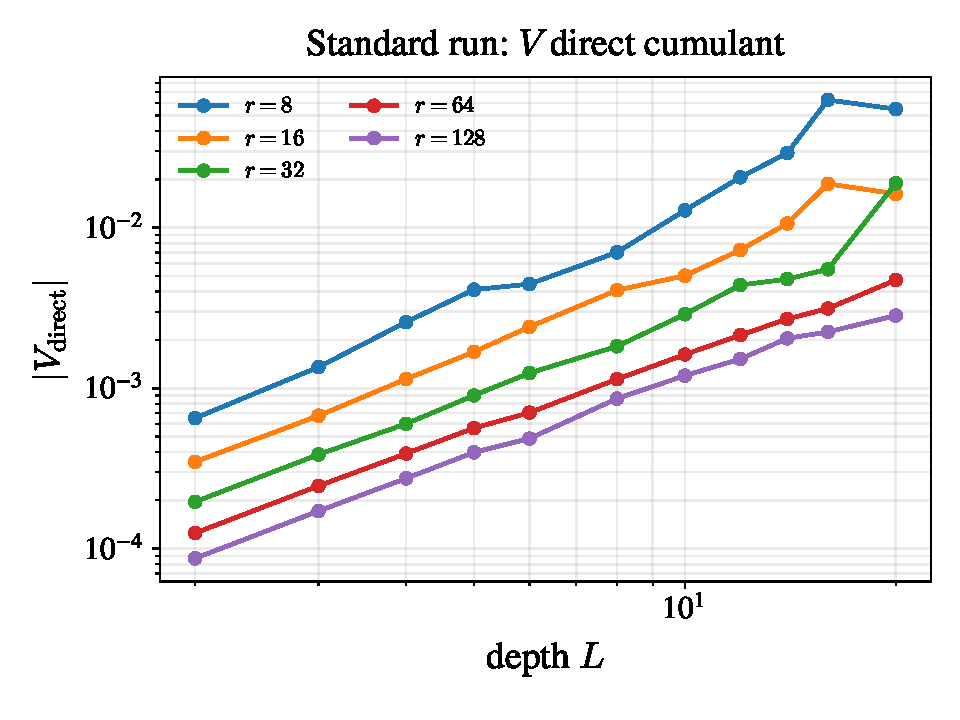
\includegraphics[width=0.92\linewidth]{../../data/feynman/true_finite_ntk_cumulants_very_long/cumulant_loglog_V_same_off.pdf}
\end{minipage}
\hfill
\begin{minipage}{0.30\linewidth}
\centering
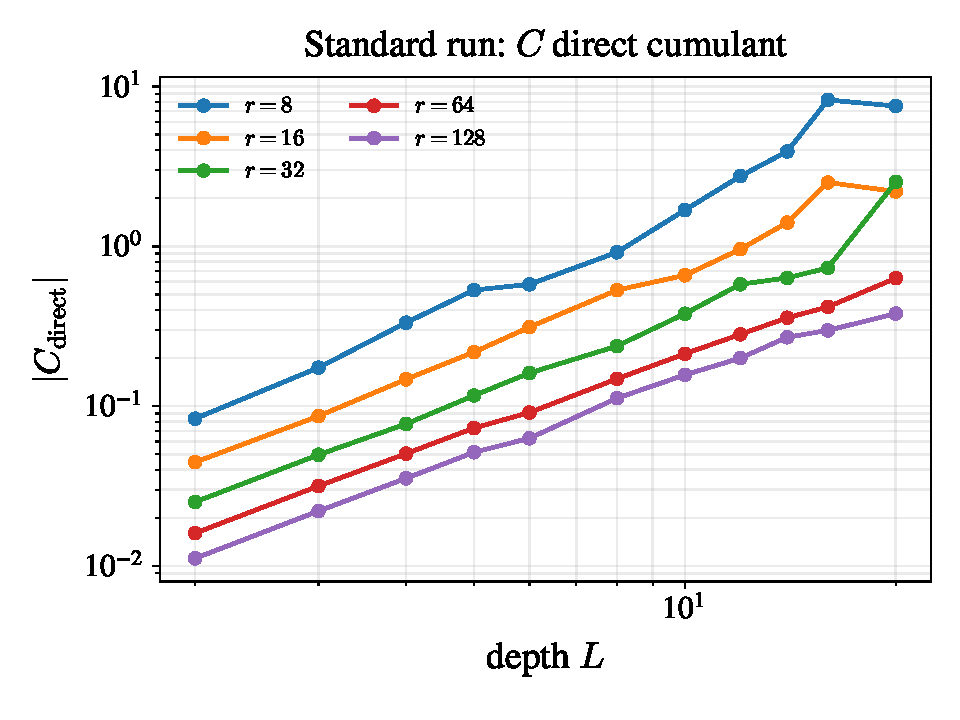
\includegraphics[width=0.92\linewidth]{../../data/feynman/true_finite_ntk_cumulants_very_long/cumulant_loglog_C_same_off.pdf}
\end{minipage}
\hfill
\begin{minipage}{0.30\linewidth}
\centering
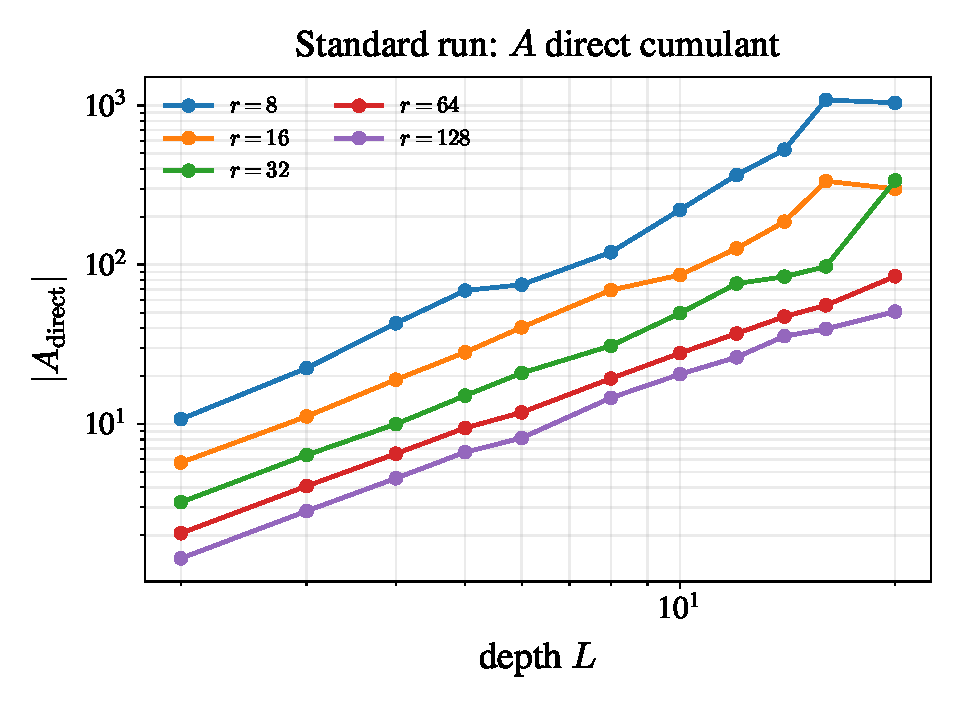
\includegraphics[width=0.92\linewidth]{../../data/feynman/true_finite_ntk_cumulants_very_long/cumulant_loglog_A_same_off.pdf}
\end{minipage}
\vspace{-0.5em}
\caption{Direct finite-network cumulant magnitudes from the standard long run. From left to right: \(V_{\mathrm{direct}}\), \(C_{\mathrm{direct}}\), and \(A_{\mathrm{direct}}\). These scalar-output observables mix several diagrammatic sectors, so their slopes are effective diagnostics rather than isolated tensor exponents.}
\label{fig:main-cumulant-loglog}
\end{figure}

\begin{table}[H]
\centering
\caption{Effective log-log depth slopes from the same standard long run as Figure \ref{fig:main-cumulant-loglog}, using \(L\in\{2,3,4,5,6,8,10,12,14,16,20\}\). These slopes are diagnostics of scalar-output contracted observables, not isolated diagrammatic tensor exponents.}
\label{tab:effective-cumulant-slopes}
\begin{tabular}{rrrr}
\toprule
Rank \(r\) & \(V_{\mathrm{direct}}\) & \(C_{\mathrm{direct}}\) & \(A_{\mathrm{direct}}\) \\
\midrule
8 & \(2.01\) & \(2.03\) & \(2.06\) \\
16 & \(1.76\) & \(1.79\) & \(1.81\) \\
32 & \(1.79\) & \(1.81\) & \(1.83\) \\
64 & \(1.56\) & \(1.58\) & \(1.59\) \\
128 & \(1.55\) & \(1.57\) & \(1.58\) \\
\bottomrule
\end{tabular}
\end{table}
For a transported off-diagonal leg, \(\lambda=3\). Indeed, the leg is multiplied from layer \(k\) to layer \(L\) by
\[
\prod_{j=k+1}^{L}\dot{\mathcal C}(\rho_j)
=\prod_{j=k+1}^{L}\left(1-\frac3j+O\left(\frac{\log j}{j^2}\right)\right)
=\left(\frac{k}{L}\right)^3(1+o(1)),
\]
because the logarithm of the product is \(-3\sum_{j=k+1}^{L}j^{-1}+O(1/k)\). This is the source of the exponent \(3\). Appendix \ref{app:proof-endpoint-constants} gives the ReLU moment and Riemann-sum calculation behind the mixed and NTK-NTK endpoint integrals:
\begin{equation}
B_\lambda=\frac1{\lambda+1}\left(5-\frac4{\lambda+2}\right),
\qquad
A_{\lambda,\mu}=\frac{1}{(\lambda+1)(\mu+1)}\left(5-\frac4{\lambda+2}-\frac4{\mu+2}+\frac4{\lambda+\mu+3}\right).
\end{equation}
Thus for off-diagonal modes,
\begin{equation}
V: 5,
\qquad
C: B_3=\frac{21}{20},
\qquad
A: A_{3,3}=\frac{173}{720}.
\label{eq:endpoint-constants}
\end{equation}
The diagonal/off-diagonal endpoint table is
\begin{center}
\begin{tabular}{lc}
\toprule
Tensor coordinate & leading coefficient \\
\midrule
\(V(e,f)\) & \(5\) \\
\(D(e,f),F(e,f)\), transported leg diagonal & \(B_0=3\) \\
\(D(e,f),F(e,f)\), transported leg off-diagonal & \(B_3=21/20\) \\
\(A(e,f),B(e,f)\), both legs diagonal & \(A_{0,0}=7/3\) \\
\(A(e,f),B(e,f)\), one diagonal and one off-diagonal leg & \(A_{0,3}=43/60\) \\
\(A(e,f),B(e,f)\), both legs off-diagonal & \(A_{3,3}=173/720\) \\
\bottomrule
\end{tabular}
\end{center}
Equivalently, for four distinct generic inputs and the three pairing vectors in \eqref{eq:V-full-dictionary}--\eqref{eq:A-full-dictionary},
\begin{align}
\mathcal V_L
&=
5\,\barE L\,\mathbf 1_3+O(\barE\log^2L),\\
\mathcal C_L
&=
\frac{21}{20}\,\barE L^2\,\mathbf 1_3+O(\barE L\log^2L),\\
\mathcal A_L
&=
\frac{173}{720}\,\barE L^3\,\mathbf 1_3+O(\barE L^2\log^2L),
\label{eq:pairing-vector-asymptotics}
\end{align}
up to the finite pairing-basis projection factors already absorbed in the \(O(\barE)\) normalization. This is the calculation from which the main \(L,L^2,L^3\) hierarchy is extracted.

\begin{figure}[H]
\centering
\begin{minipage}{0.235\linewidth}
\centering
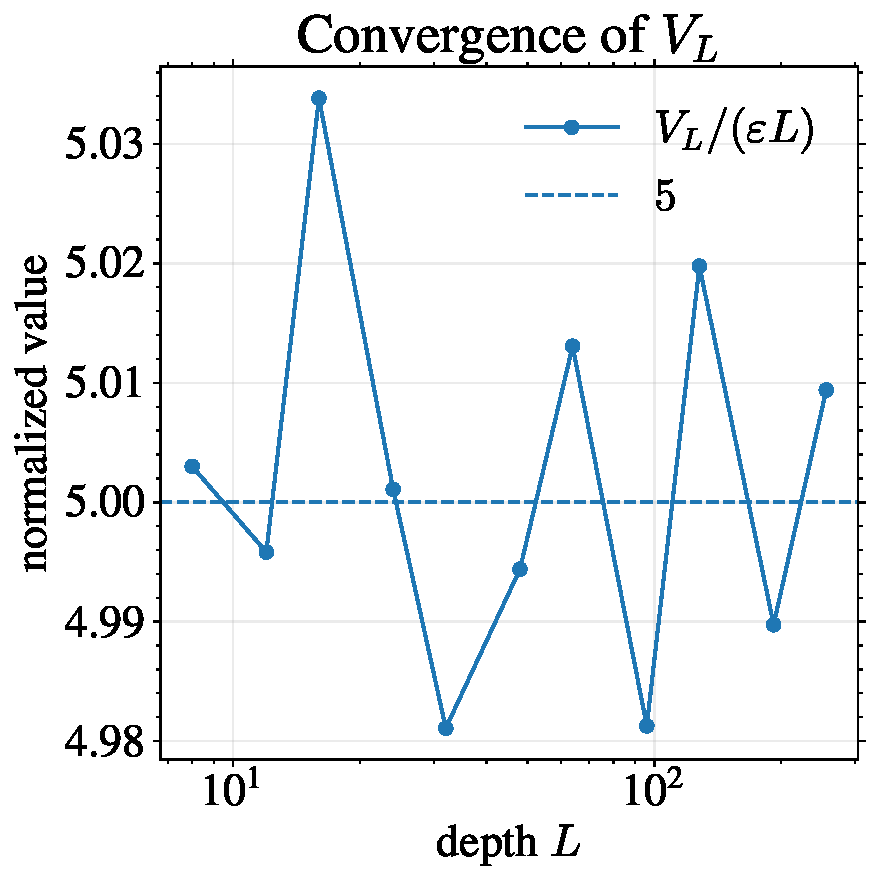
\includegraphics[width=0.92\linewidth]{../../data/feynman/lowrank_ntk_proxy_outputs_clean/convergence_V.pdf}
\end{minipage}
\hfill
\begin{minipage}{0.235\linewidth}
\centering
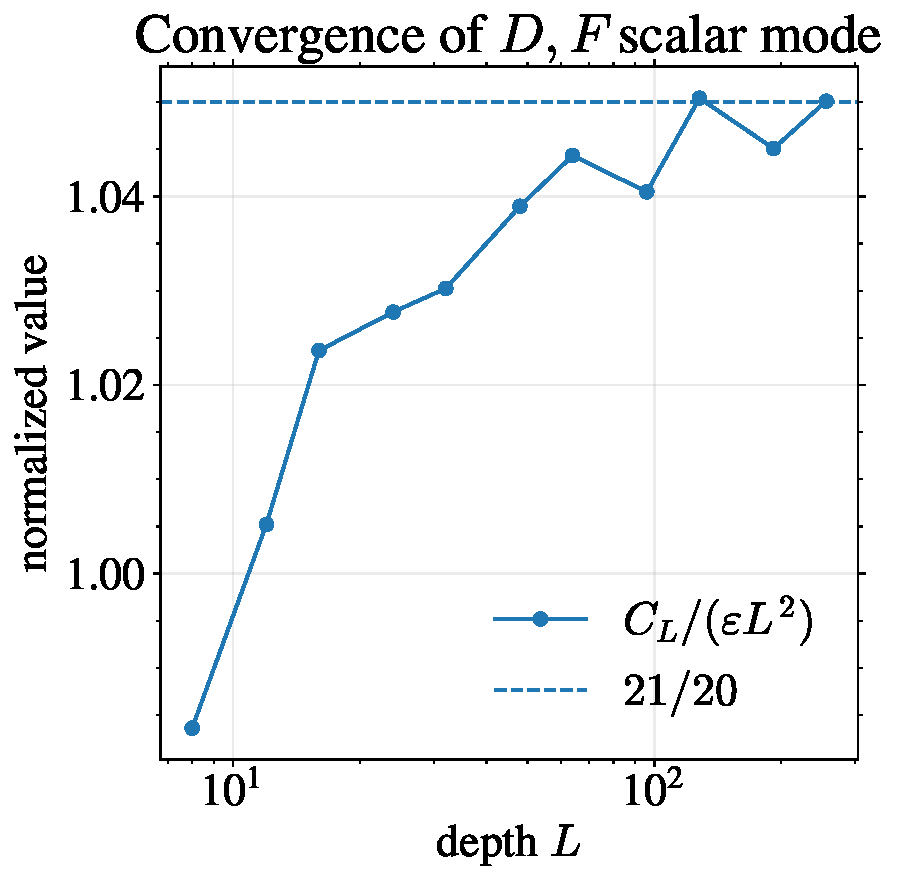
\includegraphics[width=0.92\linewidth]{../../data/feynman/lowrank_ntk_proxy_outputs_clean/convergence_C.pdf}
\end{minipage}
\hfill
\begin{minipage}{0.235\linewidth}
\centering
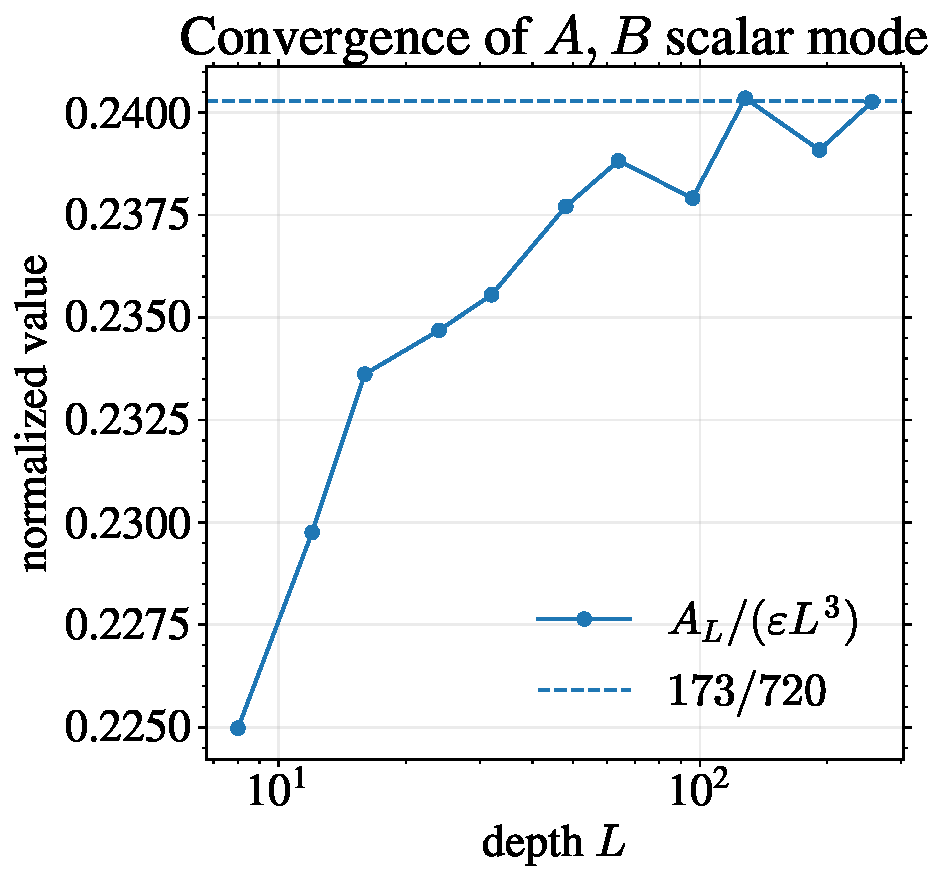
\includegraphics[width=0.92\linewidth]{../../data/feynman/lowrank_ntk_proxy_outputs_clean/convergence_A.pdf}
\end{minipage}
\hfill
\begin{minipage}{0.235\linewidth}
\centering
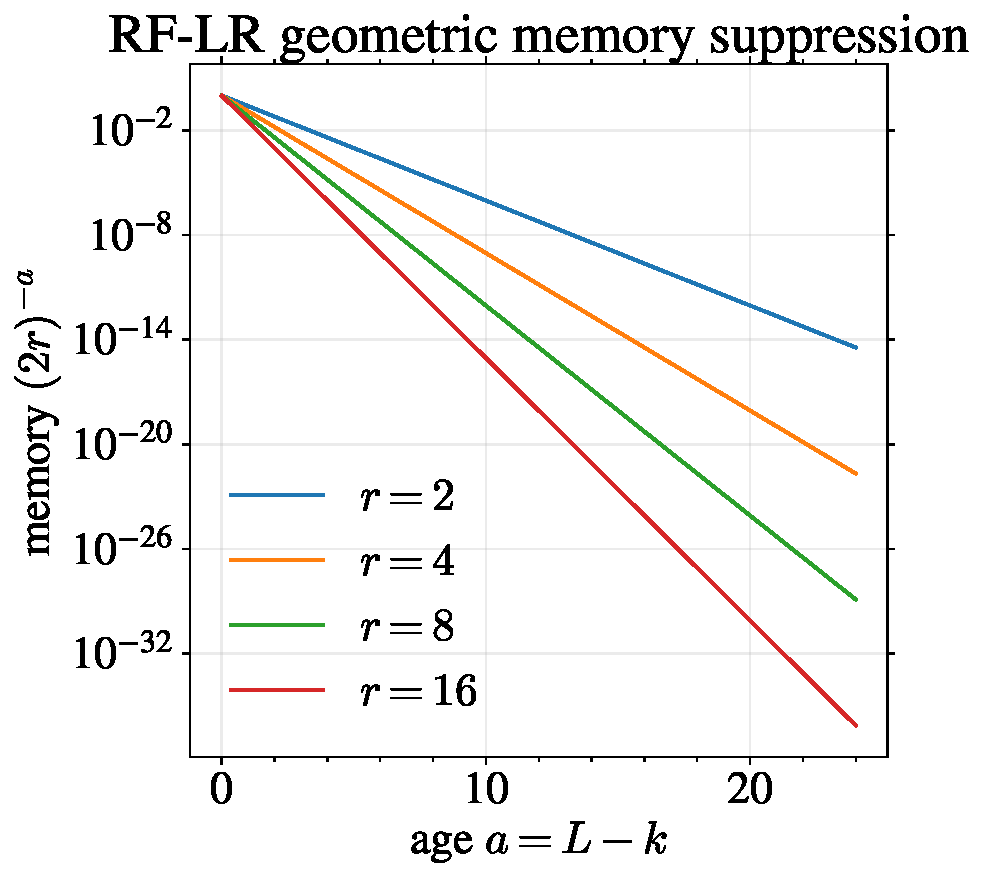
\includegraphics[width=0.92\linewidth]{../../data/feynman/lowrank_ntk_proxy_outputs_clean/rflr_memory_suppression.pdf}
\end{minipage}
\vspace{-0.5em}
\caption{Tensor constants and RF-LR memory. The first three panels show convergence to the isolated constants \(5\), \(21/20\), and \(173/720\). The last panel shows geometric suppression of old NTK memory in the RF-LR bottleneck.}
\label{fig:proxy-constants}
\end{figure}

These constants are tensor coefficients after pairing-basis extraction, not arbitrary scalar-output cumulants. Direct finite-network cumulants mix Wick/Wishart terms, radial modes, readout contractions, and several Feynman sectors; Appendix \ref{app:extended-experiments} reports the corresponding log-log diagnostics.

\iffalse
\subsection{A three-layer finite-rank calculation}
The simplest place where the low-rank simplification is visible is a three-layer network, i.e. two ReLU feature maps. Let
\[
Q_x=\frac1r\sum_{a=1}^{r}X_a^2,\qquad
Q_y=\frac1r\sum_{a=1}^{r}Y_a^2,\qquad
S=\frac1r\sum_{a=1}^{r}X_aY_a,
\qquad
C_r=\frac{S}{\sqrt{Q_xQ_y}}.
\]
For the right-factor-only low-rank model, the empirical second hidden-layer kernel has the schematic form
\[
K_{2,r}=\sqrt{Q_xQ_y}\,\kappa(C_r),
\qquad
\dot K_{2,r}=\dot\kappa(C_r),
\qquad
\wh\Theta^{(3)}_r=K_{2,r}+S\,\dot K_{2,r},
\]
where \(\kappa\) is the normalized ReLU covariance map.

\begin{proposition}[Delta-method correction for three layers]
\label{prop:three-layer-delta}
For fixed correlation \(\rho\in(-1,1)\), there is an explicit smooth function \(\Delta^{(3)}(\rho)\), depending only on \(\kappa,\dot\kappa\) and the covariance matrix of \((X^2,Y^2,XY)\), such that
\begin{equation}
\E\,\wh\Theta^{(3)}_r(\rho)
=\Theta^{(3)}_\infty(\rho)+\frac1r\Delta^{(3)}(\rho)+O(r^{-2}),
\qquad
\wh\Theta^{(3)}_r-\E\wh\Theta^{(3)}_r=O_{\Pp}(r^{-1/2}).
\label{eq:three-layer-delta}
\end{equation}
For scale-invariant ReLU on the diagonal, \(\Delta^{(3)}(1)=0\).
\end{proposition}

\begin{proof}
Write \(\wh\Theta^{(3)}_r=F(Q_x,Q_y,S)\). By the multivariate central limit theorem and Lemma \ref{lem:rank-cumulant-counting},
\[
(Q_x,Q_y,S)=(1,1,\rho)+r^{-1/2}\xi+O_{\Pp}(r^{-1})
\]
with \(\xi\) asymptotically Gaussian and covariance determined by the moments of \((X^2,Y^2,XY)\). Taylor expansion gives
\[
\E F(Q_x,Q_y,S)
=F(1,1,\rho)+\frac1{2r}\tr\left(\nabla^2F(1,1,\rho)\,\Sigma_\rho\right)+O(r^{-2}),
\]
which is \eqref{eq:three-layer-delta}. The \(O_{\Pp}(r^{-1/2})\) fluctuation is the first-order delta-method term. On the diagonal \(X=Y\), ReLU scale invariance makes the normalized correlation and derivative atoms deterministic along the radial direction, cancelling the first mean correction.
\end{proof}
\fi

A concrete three-layer delta-method calculation is given in Appendix \ref{app:three-layer-delta}. It shows explicitly that right-factor-only low rank produces an \(r^{-1}\) mean correction and \(r^{-1/2}\) single-seed fluctuations, while the diagonal ReLU correction cancels by scale invariance.

\section{Operator Concentration and Spectral Preservation}
The previous tensor estimates control individual NTK entries. For training stability, the relevant question is stronger: whether the whole empirical NTK matrix stays close enough to its limiting kernel that its smallest useful eigenvalue remains positive.
Let \(\Theta_{\infty,L}\) be the deterministic limiting NTK and \(\wh\Theta_L\) the empirical finite NTK. Entrywise tensor bounds give
\begin{equation}
\Var((\wh\Theta_L)_{ab})\lesssim L^3\barE,
\qquad
|\E(\wh\Theta_L)_{ab}-(\Theta_{\infty,L})_{ab}|\lesssim L^3\barE.
\end{equation}
A layer martingale and Matrix Freedman yield the operator form. Matrix Freedman is the matrix-valued analogue of Freedman's martingale concentration inequality: it controls the operator norm of a sum of conditionally mean-zero random matrices using a bound on the largest increment and on the predictable quadratic variation. The well-spread data assumption below means that no small group of examples dominates the random feature directions; equivalently, the matrix variance of the empirical NTK fluctuation grows like \(m\), not \(m^2\). This is not true for every deterministic dataset: duplicated, nearly duplicated, or highly aligned examples can violate it. It is a standard incoherence-type assumption, and it holds with high probability for many random generic datasets, for example iid sub-Gaussian or spherical inputs with bounded aspect ratio and no near-collisions, but we keep it explicit rather than hiding it inside the theorem.

\begin{theorem}[Finite-network operator concentration]
\label{thm:operator}
Assume \(L^3\barE\le c\). Assume further that the data are well-spread in the layerwise feature bases, so the entrywise tensor variance bounds upgrade to a matrix variance proxy of order \(mL^3\barE\). With probability at least \(1-\delta\),
\begin{equation}
\|\wh\Theta_L-\Theta_{\infty,L}\|_{\op}
\le
C L^{3/2}\sqrt{m\barE}\,\operatorname{polylog}(m,L,1/\delta)
+C mL^3\barE\,\operatorname{polylog}(m,L,1/\delta).
\label{eq:operator-bound}
\end{equation}
Without the well-spread data assumption, the same argument still gives a robust bound, but the variance term is weaker:
\[
C L^{3/2}\sqrt{m\barE}
\quad\text{is replaced by}\quad
C mL^{3/2}\sqrt{\barE}.
\]
The deterministic bias term \(C mL^3\barE\) is unchanged.
\end{theorem}

\begin{proof}[Proof sketch]
Expose the random weights and projectors layer by layer and decompose \(\wh\Theta_L-\E\wh\Theta_L\) as a matrix martingale. Proposition \ref{prop:tensor-hierarchy} gives conditional entrywise variance \(O(L^3\barE)\) and conditional bias \(O(L^3\barE)\). Under the well-spread data assumption, the predictable quadratic variation is \(O(mL^3\barE)\) in operator norm rather than \(O(m^2L^3\barE)\). Matrix Freedman gives the first term in \eqref{eq:operator-bound}, with logarithmic losses from truncation and union over tensor coordinates. The deterministic bias contributes the second term. Without this assumption, the same argument uses the Frobenius-to-operator bound on the variance proxy and loses a factor \(\sqrt m\).
\end{proof}

If \(\mu_\infty(L)=\lambda_{\min}(P_m\Theta_{\infty,L}P_m)\) is the limiting centered spectral margin, Weyl's inequality gives preservation whenever the right-hand side of \eqref{eq:operator-bound} is at most \(\mu_\infty(L)/2\). In the RF-LR bottleneck, the baseline is not the dense MLP margin; the centered proxy margin can scale as \(1/(rL)\). Combining this with the bottleneck deviation gives the conservative design rule \(r\gtrsim mL^3\), up to logarithmic factors, when the RF-LR perturbation scale is \(1/r\).

\subsection{RF-LR memory and rank-depth rules}
The RF-LR recursion \eqref{eq:rflr-recursion} is not a full-rank-compatible perturbation. Its old-kernel memory obeys an exact product rule:
\begin{equation}
\Theta^{(L)}_{\mathrm{old}\leftarrow k}
=\Theta^{(k)}\prod_{j=k+1}^{L}\frac{\dot\Sigma^{(j)}}{r}.
\label{eq:rflr-memory-product}
\end{equation}
At the normalized ReLU edge of chaos, \(\dot\Sigma^{(j)}=1/2+O(j^{-1})\), hence
\begin{equation}
\left|\Theta^{(L)}_{\mathrm{old}\leftarrow k}\right|
\le C\left(\frac1{2r}\right)^{L-k}\left(\frac{L}{k}\right)^C.
\label{eq:rflr-memory-bound}
\end{equation}
Low rank therefore shortens old NTK memory geometrically. The cost is that the centered deterministic margin can shrink with \(r\) and \(L\).

\begin{proposition}[Unprojected and centered RF-LR stability rules]
\label{prop:rflr-rules}
Consider an RF-LR bottleneck whose centered limiting margin satisfies
\(\mu_{\mathrm{RF}}(L,r)\gtrsim (rL)^{-1}\). If the empirical operator deviation is controlled by the conservative scale \(L^{3/2}\sqrt{m/r}+mL^3/r\), then spectral preservation follows from
\begin{equation}
r\gtrsim mL^3\,\operatorname{polylog}(m,L,1/\delta).
\label{eq:rflr-unprojected-rule}
\end{equation}
If the radial mode is projected out and an angularized centered decomposition improves the variance scale by one power of \(L\), then the sufficient rule improves to
\begin{equation}
r\gtrsim mL^2\,\operatorname{polylog}(m,L,1/\delta).
\label{eq:rflr-centered-rule}
\end{equation}
\end{proposition}

\begin{proof}
Weyl's inequality requires the operator deviation to be at most a fixed fraction of \(\mu_{\mathrm{RF}}(L,r)\). In the unprojected RF-LR model, the radial contribution remains present in the \(A\)-sector, whose tensor scale is cubic in depth. The sufficient inequality is therefore dominated by the \(mL^3/r\) contribution after absorbing logarithms and constants, giving \eqref{eq:rflr-unprojected-rule}. In the centered/angularized model, the radial sector is removed before concentration and the dominant tensor variance is quadratic in depth. Repeating the same Weyl argument gives \eqref{eq:rflr-centered-rule}. The second statement is conditional on this projection and should not be read as the default RF-LR rule.
\end{proof}

\iffalse
\section{NTK Descendants and Training-Time Drift}
This section checks that dNTK and ddNTK objects use the same probabilistic vertices, so training-time NTK drift does not introduce a new low-rank random mechanism.
Let \(J_c=\nabla_\theta f(x_c)\) and define the dNTK and ddNTK descendants
\begin{equation}
\Xi_{ab;c}=D\Theta_{ab}[J_c],
\qquad
\Psi_{ab;cd}=D^2\Theta_{ab}[J_c,J_d].
\end{equation}
These descendants add derivative legs to the same layer maps. They do not introduce new independent random variables.

\begin{proposition}[No new low-rank vertices]
\label{prop:no-new-vertices}
The joint cumulants of \((K,\Theta,\Xi,\Psi)\) are generated by the same Gaussian-ReLU atoms and Stiefel-projector cumulants of \(G=(n/r)UU^\top\). Differentiation changes deterministic contractions but not the probabilistic vertex set.
\end{proposition}

\begin{proof}
Each derivative of the network output with respect to a trainable right factor \(B^{(\ell)}\) inserts an additional deterministic backpropagated leg and a factor of the same frozen projector \(UU^\top\). Higher derivatives differentiate ReLU gates and covariance maps, changing the local deterministic tensors \(\kappa,\dot\kappa,\ddot\kappa\), but all randomness still comes from the original Gaussian preactivations, readout weights, and frozen projectors. Since \(U\) is fixed, there is no moving-projector derivative. Thus the connected diagrams for \(K,\Theta,\Xi,\Psi\) have the same random vertices as the NTK diagrams and only differ in their deterministic leg labels.
\end{proof}

Under square-loss gradient flow, \(\dot\Theta_{ab,t}=-\sum_c\Xi_{ab;c,t}e_{c,t}\). The descendant concentration bound therefore yields, in a lazy window,
\begin{equation}
\|\Theta_t-\Theta_0\|_{\op}
\le
C t\|e_0\|_2\left(L^3\sqrt{m\barE}+mL^3\barE\right)\operatorname{polylog}(m,L,1/\delta).
\end{equation}
\fi

\paragraph{Training-time drift.}
dNTK and ddNTK descendants use the same Gaussian-ReLU atoms and Stiefel-projector cumulants as the NTK itself; differentiation changes deterministic leg labels, not the low-rank random vertex set. The full statement is in Appendix \ref{app:ntk-descendants}.

\paragraph{Experiments.}
The main figures above give the projector, tensor-constant, memory, and slope diagnostics next to the claims they support. Appendix \ref{app:extended-experiments} reports the remaining true finite-network empirical NTKs, the deep cumulant stress test, and exact full-rank matching.

The true finite-network NTK plots, log-log cumulant panels, effective slope table, and depth-\(200\) full-rank matching table are reported in Appendix \ref{app:extended-experiments}. They support the same claims: operator deviations follow the predicted normalization, finite-network cumulants exhibit polynomial effective slopes, and the full-rank endpoint matches the dense NTK to numerical precision.

\FloatBarrier

\section{Conclusion}
Low rank changes finite-width NTK theory not only by reducing parameters, but by changing the stability threshold for training. The MLP-compatible model isolates full-rank-compatible rank defects, whereas RF-LR bottlenecks suppress old NTK memory by approximately \((2r)^{-(L-k)}\) while also shrinking the centered deterministic gap. Combining these effects gives the main design message: preserving the NTK edge of convexity has a conservative cubic-depth sufficient rule, \(r\gtrsim mL^3\), up to logarithmic factors. The experiments do not contradict this theorem; they show that scalar-output contracted observables can have smaller effective exponents, around \(1.5\)--\(2.1\), suggesting a sharper mode-dependent law between \(L^{3/2}\) and \(L^2\). The rank-width diagrammatics developed here connect these criteria to conditional operator concentration and to finite-network experiments.

The consequence is that rank should be treated as a stability budget, not only as a compression knob. If the rank is too small, the model may still have fewer parameters, but its empirical NTK can drift far enough from the dense geometry to lose the spectral margin that makes lazy training predictable. The results also explain why full-rank factorization is harmless, why RF-LR bottlenecks behave differently, and why finite-network experiments can show milder effective depth laws than the conservative theorem. In practice, the theory gives a cautious certificate: it identifies when low rank is expected to preserve the optimization geometry, and where sharper mode-dependent predictions are still needed.

To our knowledge, this is the first framework that reconciles low-rank feature geometry with an NTK convexity certificate: low rank can select interpretable bottleneck features while still preserving the spectral conditions that make lazy training predictable.

\clearpage
\begin{thebibliography}{99}
\bibitem{Jacot2018}
A. Jacot, F. Gabriel, and C. Hongler.
\newblock Neural tangent kernel: convergence and generalization in neural networks.
\newblock \emph{NeurIPS}, 2018.

\bibitem{Lee2019}
J. Lee, L. Xiao, S. Schoenholz, Y. Bahri, J. Sohl-Dickstein, and J. Pennington.
\newblock Wide neural networks of any depth evolve as linear models under gradient descent.
\newblock \emph{NeurIPS}, 2019.

\bibitem{Du2019}
S. Du, J. Lee, H. Li, L. Wang, and X. Zhai.
\newblock Gradient descent finds global minima of deep neural networks.
\newblock \emph{ICML}, 2019.

\bibitem{AllenZhu2019}
Z. Allen-Zhu, Y. Li, and Z. Song.
\newblock A convergence theory for deep learning via over-parameterization.
\newblock \emph{ICML}, 2019.

\bibitem{Arora2019}
S. Arora, S. Du, W. Hu, Z. Li, R. Salakhutdinov, and R. Wang.
\newblock On exact computation with an infinitely wide neural net.
\newblock \emph{NeurIPS}, 2019.

\bibitem{NguyenMondelli2020}
Q. Nguyen and M. Mondelli.
\newblock Global convergence of deep networks with one wide layer followed by pyramidal topology.
\newblock \emph{NeurIPS}, 2020.

\bibitem{NguyenMondelliMontufar2022}
Q. Nguyen, M. Mondelli, and G. Montúfar.
\newblock Tight bounds on the smallest eigenvalue of the neural tangent kernel for deep ReLU networks.
\newblock \emph{ICML}, 2021.

\bibitem{TerjekGonzalezSanchez2025Concentration}
D. Terjék and D. González-Sánchez.
\newblock MLPs at the EOC: Concentration of the NTK.
\newblock arXiv:2501.14724, 2025.

\bibitem{TerjekGonzalezSanchez2025Spectrum}
D. Terjék and D. González-Sánchez.
\newblock MLPs at the EOC: Spectrum of the NTK.
\newblock arXiv:2501.13225, 2025.

\bibitem{Yang2019}
G. Yang.
\newblock Wide feedforward or recurrent neural networks of any architecture are Gaussian processes.
\newblock \emph{NeurIPS}, 2019.

\bibitem{Yang2021}
G. Yang and E. Hu.
\newblock Tensor programs IV: Feature learning in infinite-width neural networks.
\newblock \emph{ICML}, 2021.

\bibitem{Yang2022MuP}
G. Yang, E. J. Hu, I. Babuschkin, S. Sidor, X. Liu, D. Farhi, N. Ryder, J. Pachocki, W. Chen, and J. Gao.
\newblock Tensor programs V: Tuning large neural networks via zero-shot hyperparameter transfer.
\newblock \emph{NeurIPS}, 2021.

\bibitem{YangDepthMuP2024}
G. Yang, D. Yu, C. Zhu, and S. Hayou.
\newblock Tensor programs VI: Feature learning in infinite-depth neural networks.
\newblock \emph{ICLR}, 2024.

\bibitem{BordelonPehlevan2022}
B. Bordelon and C. Pehlevan.
\newblock Self-consistent dynamical field theory of kernel evolution in wide neural networks.
\newblock \emph{NeurIPS}, 2022.

\bibitem{MeiMontanariNguyen2018}
S. Mei, A. Montanari, and P.-M. Nguyen.
\newblock A mean field view of the landscape of two-layer neural networks.
\newblock \emph{PNAS}, 2018.

\bibitem{ChizatBach2018}
L. Chizat and F. Bach.
\newblock On the global convergence of gradient descent for over-parameterized models using optimal transport.
\newblock \emph{NeurIPS}, 2018.

\bibitem{RotskoffVandenEijnden2018}
G. M. Rotskoff and E. Vanden-Eijnden.
\newblock Neural networks as interacting particle systems: Asymptotic convexity of the loss landscape and universal scaling of the approximation error.
\newblock arXiv:1805.00915, 2018.

\bibitem{Huang2020}
J. Huang and H.-T. Yau.
\newblock Dynamics of deep neural networks and neural tangent hierarchy.
\newblock \emph{ICML}, 2020.

\bibitem{DyerGurAri2019}
E. Dyer and G. Gur-Ari.
\newblock Asymptotics of wide networks from Feynman diagrams.
\newblock arXiv:1909.11304, 2019.

\bibitem{FeynmanNTK2025}
M. Guillen, P. Misof, and J. E. Gerken.
\newblock Finite-width neural tangent kernels from Feynman diagrams.
\newblock arXiv:2508.11522, 2025.

\bibitem{Novak2022}
R. Novak, J. Sohl-Dickstein, and S. Schoenholz.
\newblock Fast finite width neural tangent kernel.
\newblock \emph{ICML}, 2022.

\bibitem{JangLeeRyu2024LoRA}
U. Jang, J. D. Lee, and E. K. Ryu.
\newblock LoRA training in the NTK regime has no spurious local minima.
\newblock \emph{ICML}, 2024.

\bibitem{MosigGarciaAgazziTrevisan2025}
E. Mosig García, A. Agazzi, and D. Trevisan.
\newblock Quantitative convergence of trained single layer neural networks to Gaussian processes.
\newblock arXiv:2509.24544, 2025.
\end{thebibliography}

\section*{NeurIPS Paper Checklist}

\begin{enumerate}[leftmargin=1.5em]

\item {\bf Claims}
    \item[] Question: Do the main claims made in the abstract and introduction accurately reflect the paper's contributions and scope?
    \item[] Answer: \answerYes{}
    \item[] Justification: The abstract and introduction state the paper's scope as a finite-width and finite-rank NTK analysis, and the assumptions are made explicit in the theorem statements. The empirical MNIST table is presented only as motivation, not as evidence for the main theoretical claims.
    \item[] Guidelines:
    \begin{itemize}
        \item The answer \answerNA{} means that the abstract and introduction do not include the claims made in the paper.
        \item The abstract and/or introduction should clearly state the claims made, including the contributions made in the paper and important assumptions and limitations. A \answerNo{} or \answerNA{} answer to this question will not be perceived well by the reviewers.
        \item The claims made should match theoretical and experimental results, and reflect how much the results can be expected to generalize to other settings.
        \item It is fine to include aspirational goals as motivation as long as it is clear that these goals are not attained by the paper.
    \end{itemize}

\item {\bf Limitations}
    \item[] Question: Does the paper discuss the limitations of the work performed by the authors?
    \item[] Answer: \answerYes{}
    \item[] Justification: The conclusion states the narrow scope of the results, including the restriction to signed/isometric low-rank factors and RF-LR bottlenecks, the status of the endpoint constants, the logarithmic losses, and the open dNTK/ddNTK coefficient problem.
    \item[] Guidelines:
    \begin{itemize}
        \item The answer \answerNA{} means that the paper has no limitation while the answer \answerNo{} means that the paper has limitations, but those are not discussed in the paper.
        \item The authors are encouraged to create a separate ``Limitations'' section in their paper.
        \item The paper should point out any strong assumptions and how robust the results are to violations of these assumptions.
        \item The authors should reflect on the scope of the claims made.
        \item The authors should reflect on the factors that influence the performance of the approach.
        \item The authors should discuss the computational efficiency of the proposed algorithms and how they scale with dataset size.
        \item If applicable, the authors should discuss possible limitations of their approach to address problems of privacy and fairness.
        \item While the authors might fear that complete honesty about limitations might be used by reviewers as grounds for rejection, reviewers will be specifically instructed to not penalize honesty concerning limitations.
    \end{itemize}

\item {\bf Theory assumptions and proofs}
    \item[] Question: For each theoretical result, does the paper provide the full set of assumptions and a complete proof?
    \item[] Answer: \answerYes{}
    \item[] Justification: The theorem, proposition, and lemma statements specify the finite-rank, projector, ReLU transport, well-spread-data, and RF-LR assumptions. Proof sketches are in the main text, with the tensor hierarchy, projector cumulants, descendant arguments, and endpoint calculations expanded in the appendices.
    \item[] Guidelines:
    \begin{itemize}
        \item The answer \answerNA{} means that the paper does not include theoretical results.
        \item All the theorems, formulas, and proofs in the paper should be numbered and cross-referenced.
        \item All assumptions should be clearly stated or referenced in the statement of any theorems.
        \item The proofs can either appear in the main paper or the supplemental material.
        \item Any informal proof provided in the core of the paper should be complemented by formal proofs provided in appendix or supplemental material.
        \item Theorems and lemmas that the proof relies upon should be properly referenced.
    \end{itemize}

\item {\bf Experimental result reproducibility}
    \item[] Question: Does the paper fully disclose all the information needed to reproduce the main experimental results of the paper?
    \item[] Answer: \answerYes{}
    \item[] Justification: Appendix \ref{app:extended-experiments} gives widths, ranks, depths, sample sizes, dimensions, repetitions, normalizations, and metrics for the true finite-network and proxy experiments. Appendix \ref{app:mnist-details} gives the MNIST architecture, optimizer, learning rate, batch size, epochs, seed, and clipping rule.
    \item[] Guidelines:
    \begin{itemize}
        \item The answer \answerNA{} means that the paper does not include experiments.
        \item If the paper includes experiments, a \answerNo{} answer to this question will not be perceived well by the reviewers.
        \item If the contribution is a dataset and\slash or model, the authors should describe the steps taken to make their results reproducible or verifiable.
        \item Reproducibility can be accomplished through code, detailed instructions, model access, or other means appropriate to the research performed.
    \end{itemize}

\item {\bf Open access to data and code}
    \item[] Question: Does the paper provide open access to the data and code, with sufficient instructions to faithfully reproduce the main experimental results, as described in supplemental material?
    \item[] Answer: \answerYes{}
    \item[] Justification: An anonymized supplemental code bundle contains the Feynman/NTK experiment scripts and the MNIST scripts, together with a README describing the contents. Synthetic data are generated by the scripts, and MNIST is downloaded through the standard dataset loader.
    \item[] Guidelines:
    \begin{itemize}
        \item The answer \answerNA{} means that paper does not include experiments requiring code.
        \item Please see the NeurIPS code and data submission guidelines for more details.
        \item While code release is encouraged, a justified \answerNo{} is acceptable.
        \item The instructions should contain the exact command and environment needed to reproduce the results.
        \item The authors should provide instructions on data access and preparation.
        \item The authors should provide scripts to reproduce all experimental results for the new proposed method and baselines.
        \item At submission time, anonymized versions should be released if applicable.
    \end{itemize}

\item {\bf Experimental setting/details}
    \item[] Question: Does the paper specify all the training and test details necessary to understand the results?
    \item[] Answer: \answerYes{}
    \item[] Justification: The appendices specify the finite-network initialization protocol, uniform Stiefel sampling, autograd NTK computation, ranks, widths, depths, sample sizes, seeds or repetition counts, and MNIST optimizer/training settings.
    \item[] Guidelines:
    \begin{itemize}
        \item The answer \answerNA{} means that the paper does not include experiments.
        \item The experimental setting should be presented in the core of the paper to a level of detail that is necessary to appreciate the results and make sense of them.
        \item The full details can be provided either with the code, in appendix, or as supplemental material.
    \end{itemize}

\item {\bf Experiment statistical significance}
    \item[] Question: Does the paper report error bars suitably and correctly defined or other appropriate information about the statistical significance of the experiments?
    \item[] Answer: \answerYes{}
    \item[] Justification: The true finite-network and proxy experiments report repeated-initialization summaries, including medians and means, with repetition counts stated in Appendix \ref{app:extended-experiments}. The MNIST snapshot is explicitly described as a compact motivating run rather than a statistical claim.
    \item[] Guidelines:
    \begin{itemize}
        \item The answer \answerNA{} means that the paper does not include experiments.
        \item The authors should answer \answerYes{} if the results are accompanied by error bars, confidence intervals, or statistical significance tests, at least for the experiments that support the main claims.
        \item The factors of variability that the error bars are capturing should be clearly stated.
        \item The method for calculating the error bars should be explained.
        \item The assumptions made should be given.
        \item It should be clear whether the error bar is the standard deviation or the standard error of the mean.
        \item For asymmetric distributions, authors should avoid misleading symmetric error bars.
        \item If error bars are reported, the text should explain how they were calculated and reference the corresponding figures or tables.
    \end{itemize}

\item {\bf Experiments compute resources}
    \item[] Question: For each experiment, does the paper provide sufficient information on the computer resources needed to reproduce the experiments?
    \item[] Answer: \answerNo{}
    \item[] Justification: The paper reports the model sizes and repetition counts but does not yet give precise hardware, memory, wall-clock time, or total compute estimates. The experiments are small PyTorch/autograd studies and MNIST runs, but the exact compute resources should be added before submission if required.
    \item[] Guidelines:
    \begin{itemize}
        \item The answer \answerNA{} means that the paper does not include experiments.
        \item The paper should indicate the type of compute workers CPU or GPU, internal cluster, or cloud provider, including relevant memory and storage.
        \item The paper should provide the amount of compute required for each of the individual experimental runs as well as estimate the total compute.
        \item The paper should disclose whether the full research project required more compute than the experiments reported in the paper.
    \end{itemize}

\item {\bf Code of ethics}
    \item[] Question: Does the research conducted in the paper conform, in every respect, with the NeurIPS Code of Ethics?
    \item[] Answer: \answerYes{}
    \item[] Justification: The work is a theoretical and diagnostic study using synthetic data and MNIST, with no human-subject study, private data, deployment, or high-risk released model.
    \item[] Guidelines:
    \begin{itemize}
        \item The answer \answerNA{} means that the authors have not reviewed the NeurIPS Code of Ethics.
        \item If the authors answer \answerNo{}, they should explain the special circumstances that require a deviation from the Code of Ethics.
        \item The authors should make sure to preserve anonymity.
    \end{itemize}

\item {\bf Broader impacts}
    \item[] Question: Does the paper discuss both potential positive societal impacts and negative societal impacts of the work performed?
    \item[] Answer: \answerNA{}
    \item[] Justification: The work is foundational NTK theory and finite-network diagnostics, with no deployed system, user-facing model, human-subject data, or direct application domain. Its plausible impact is indirect, through better understanding of efficient low-rank training.
    \item[] Guidelines:
    \begin{itemize}
        \item The answer \answerNA{} means that there is no societal impact of the work performed.
        \item If the authors answer \answerNA{} or \answerNo{}, they should explain why their work has no societal impact or why the paper does not address societal impact.
        \item Examples of negative societal impacts include malicious or unintended uses, fairness considerations, privacy considerations, and security considerations.
        \item The conference expects that many papers will be foundational research and not tied to particular applications.
        \item The authors should consider possible harms from intended use, incorrect results, and misuse.
        \item If there are negative societal impacts, authors may discuss mitigation strategies.
    \end{itemize}

\item {\bf Safeguards}
    \item[] Question: Does the paper describe safeguards that have been put in place for responsible release of data or models that have a high risk for misuse?
    \item[] Answer: \answerNA{}
    \item[] Justification: The paper does not release a high-risk dataset or model. The released material is code for synthetic NTK diagnostics and a standard MNIST benchmark.
    \item[] Guidelines:
    \begin{itemize}
        \item The answer \answerNA{} means that the paper poses no such risks.
        \item Released models that have a high risk for misuse or dual-use should be released with necessary safeguards.
        \item Datasets scraped from the Internet could pose safety risks.
        \item Many papers do not require safeguards, but authors should make a best faith effort.
    \end{itemize}

\item {\bf Licenses for existing assets}
    \item[] Question: Are the creators or original owners of assets used in the paper properly credited and are the license and terms of use explicitly mentioned and properly respected?
    \item[] Answer: \answerNo{}
    \item[] Justification: The paper uses MNIST through standard loaders and does not redistribute the dataset, but the current manuscript does not explicitly list MNIST license terms. This should be added to the final supplemental documentation if strict asset-license disclosure is required.
    \item[] Guidelines:
    \begin{itemize}
        \item The answer \answerNA{} means that the paper does not use existing assets.
        \item The authors should cite the original paper that produced the code package or dataset.
        \item The authors should state which version of the asset is used and, if possible, include a URL.
        \item The name of the license should be included for each asset.
        \item For scraped data, copyright and terms of service should be provided.
        \item If assets are released, license, copyright information, and terms of use should be provided.
        \item For existing datasets that are re-packaged, both the original and derived licenses should be provided.
        \item If this information is not available online, authors are encouraged to reach out to the asset's creators.
    \end{itemize}

\item {\bf New assets}
    \item[] Question: Are new assets introduced in the paper well documented and is the documentation provided alongside the assets?
    \item[] Answer: \answerYes{}
    \item[] Justification: The new supplemental asset is the experiment-code bundle, documented by a README that lists the Feynman/NTK scripts, MNIST scripts, and compact result files.
    \item[] Guidelines:
    \begin{itemize}
        \item The answer \answerNA{} means that the paper does not release new assets.
        \item Researchers should communicate the details of the dataset\slash code\slash model as part of their submissions via structured templates.
        \item The paper should discuss whether and how consent was obtained from people whose asset is used.
        \item At submission time, remember to anonymize your assets if applicable.
    \end{itemize}

\item {\bf Crowdsourcing and research with human subjects}
    \item[] Question: For crowdsourcing experiments and research with human subjects, does the paper include the full text of instructions given to participants and screenshots, if applicable, as well as details about compensation?
    \item[] Answer: \answerNA{}
    \item[] Justification: The paper does not involve crowdsourcing or human-subject research.
    \item[] Guidelines:
    \begin{itemize}
        \item The answer \answerNA{} means that the paper does not involve crowdsourcing nor research with human subjects.
        \item Including this information in the supplemental material is fine.
        \item According to the NeurIPS Code of Ethics, workers involved in data collection, curation, or other labor should be paid at least the minimum wage in the country of the data collector.
    \end{itemize}

\item {\bf Institutional review board (IRB) approvals or equivalent for research with human subjects}
    \item[] Question: Does the paper describe potential risks incurred by study participants, whether such risks were disclosed to the subjects, and whether Institutional Review Board approvals or equivalent approvals were obtained?
    \item[] Answer: \answerNA{}
    \item[] Justification: The paper does not involve crowdsourcing or human-subject research, so IRB approval is not applicable.
    \item[] Guidelines:
    \begin{itemize}
        \item The answer \answerNA{} means that the paper does not involve crowdsourcing nor research with human subjects.
        \item Depending on the country in which research is conducted, IRB approval may be required for human-subject research.
        \item Procedures may vary significantly between institutions and locations.
        \item For initial submissions, do not include any information that would break anonymity.
    \end{itemize}

\item {\bf Declaration of LLM usage}
    \item[] Question: Does the paper describe the usage of LLMs if it is an important, original, or non-standard component of the core methods in this research?
    \item[] Answer: \answerNA{}
    \item[] Justification: LLMs are not an important, original, or non-standard component of the mathematical methods, experiments, or scientific conclusions.
    \item[] Guidelines:
    \begin{itemize}
        \item The answer \answerNA{} means that the core method development in this research does not involve LLMs as any important, original, or non-standard components.
        \item Please refer to the NeurIPS LLM policy for what should or should not be described.
    \end{itemize}

\end{enumerate}

\FloatBarrier
\appendix
\renewcommand{\theHfigure}{appendix.\arabic{figure}}
\renewcommand{\theHtable}{appendix.\arabic{table}}

\section{Proof Details for Transport and Tensor Hierarchy}
\label{app:transport-hierarchy-proof}
This appendix gives the full proof behind Lemma \ref{lem:transport-source} and Proposition \ref{prop:tensor-hierarchy}. The main text keeps only the proof idea.

\paragraph{Proof of Lemma \ref{lem:transport-source}.}
Write
\[
A_\ell:=I-\frac{M}{\ell}+E_\ell,
\qquad
\Phi_{L,k}:=A_{L-1}A_{L-2}\cdots A_k
\quad (L>k),
\]
and \(\Phi_{k,k}:=I\). Since \(T_2=0\), iteration of \eqref{eq:transport-source-recursion} gives the exact variation-of-constants identity
\begin{equation}
T_L
=
\sum_{k=2}^{L-1}\Phi_{L,k+1}\,k^\beta(s+e_k).
\label{eq:appendix-voc}
\end{equation}
Let \(\Phi^0_{L,k}\) denote the unperturbed product with \(E_\ell=0\). Standard finite-dimensional product estimates for regularly varying matrix products give
\begin{equation}
\Phi^0_{L,k+1}
=
\exp\!\left(-M\sum_{j=k+1}^{L-1}\log\left(1+\frac1j\right)\right)
\left(I+O(k^{-1})\right)
=
L^{-M}k^{M}+O\!\left(L^{-M}k^{M-1}\right),
\label{eq:appendix-unperturbed-product}
\end{equation}
uniformly for \(2\le k<L\), with the usual harmless logarithmic enlargement when \(M\) is not diagonalizable. The perturbation is summable:
\[
\sum_{\ell\ge2}\|E_\ell\|
\le
C\sum_{\ell\ge2}\frac{\log^p\ell}{\ell^2}
<\infty.
\]
Discrete Duhamel expansion of the product,
\[
\Phi_{L,k+1}-\Phi^0_{L,k+1}
=
\sum_{j=k+1}^{L-1}
\Phi_{L,j+1}E_j\Phi^0_{j,k+1},
\]
together with \eqref{eq:appendix-unperturbed-product} and the summability of \(E_j\), yields
\begin{equation}
\Phi_{L,k+1}
=
L^{-M}k^M+R_{L,k},
\qquad
\sum_{k=2}^{L-1} k^\beta\|R_{L,k}\|
=
O\!\left(L^\beta\log^{p+2}L\right).
\label{eq:appendix-transport-product}
\end{equation}
Substituting \eqref{eq:appendix-transport-product} into \eqref{eq:appendix-voc} gives
\begin{equation}
T_L
=
L^{-M}\sum_{k=2}^{L-1}k^{M+\beta I}s
+O\!\left(L^\beta\log^{p+2}L\right)
+L^{-M}\sum_{k=2}^{L-1}k^{M+\beta I}e_k
+O\!\left(L^\beta\log^{p+q+2}L\right).
\label{eq:appendix-transport-sum}
\end{equation}
The error from \(e_k\) is \(O(L^\beta\log^{q+1}L)\), hence is absorbed by the displayed remainder. The spectral assumption \(\Re\lambda(M)>-(\beta+1)\) makes the matrix Riemann integral convergent. Euler-Maclaurin summation for matrix powers gives
\begin{equation}
L^{-M}\sum_{k=2}^{L-1}k^{M+\beta I}
=
L^{\beta+1}\int_0^1 u^{M+\beta I}\,\dd u
+O(L^\beta\log L).
\label{eq:appendix-matrix-riemann}
\end{equation}
Since
\[
\int_0^1 u^{M+\beta I}\,\dd u
=
\left(M+(\beta+1)I\right)^{-1},
\]
we obtain \eqref{eq:transport-source-solution}. This proves the lemma.

\paragraph{Proof of Proposition \ref{prop:tensor-hierarchy}.}
The diagrammatic recursion closes on the three blocks
\[
\mathcal V_\ell,\qquad \mathcal C_\ell=(D_\ell,F_\ell),\qquad \mathcal A_\ell=(A_\ell,B_\ell).
\]
The ReLU transport assumptions imply deterministic block recursions of the form
\begin{align}
\mathcal V_{\ell+1}
&=
\left(I-\frac{M_V}{\ell}+E^V_\ell\right)\mathcal V_\ell
+\Xi^V_\ell,
\label{eq:appendix-rigorous-V}\\
\mathcal C_{\ell+1}
&=
\left(I-\frac{M_C}{\ell}+E^C_\ell\right)\mathcal C_\ell
+B^C_\ell\mathcal V_\ell
+\Xi^C_\ell,
\label{eq:appendix-rigorous-C}\\
\mathcal A_{\ell+1}
&=
\left(I-\frac{M_A}{\ell}+E^A_\ell\right)\mathcal A_\ell
+B^A_\ell\mathcal C_\ell
+Q^A_\ell[\mathcal V_\ell,\mathcal V_\ell]
+\Xi^A_\ell,
\label{eq:appendix-rigorous-A}
\end{align}
where each \(E^*_l\) satisfies the summable bound in Lemma \ref{lem:transport-source}. The source tensors \(\Xi^V,\Xi^C,\Xi^A\) are connected rank-state or projector vertices. By Lemma \ref{lem:rank-cumulant-counting} and Lemma \ref{lem:stiefel-cov}, their second-order size is bounded by \(C\barE\) uniformly in \(\ell\):
\begin{equation}
\|\Xi^V_\ell\|+\|\Xi^C_\ell\|+\|\Xi^A_\ell\|
\le C\barE.
\label{eq:appendix-source-bound}
\end{equation}
The deterministic feed-through maps are uniformly bounded in the pairing basis, and the off-diagonal NTK transport contributes one power of \(\ell\) per transported NTK leg after summation. Equivalently, the source exponents entering Lemma \ref{lem:transport-source} are \(\beta=0\) for \(\mathcal V\), \(\beta=1\) for \(\mathcal C\), and \(\beta=2\) for \(\mathcal A\).

For \(\mathcal V\), \eqref{eq:appendix-rigorous-V} and \eqref{eq:appendix-source-bound} give Lemma \ref{lem:transport-source} with \(\beta=0\), hence
\[
\|\mathcal V_L\|\le C\barE L.
\]
For \(\mathcal C\), the effective source in \eqref{eq:appendix-rigorous-C} is \(B^C_\ell\mathcal V_\ell+\Xi^C_\ell\). The bound on \(\mathcal V_\ell\) gives
\[
\|B^C_\ell\mathcal V_\ell+\Xi^C_\ell\|
\le C\barE \ell,
\]
so Lemma \ref{lem:transport-source} with \(\beta=1\) yields
\[
\|\mathcal C_L\|\le C\barE L^2.
\]
For \(\mathcal A\), the effective source in \eqref{eq:appendix-rigorous-A} is
\[
B^A_\ell\mathcal C_\ell
+Q^A_\ell[\mathcal V_\ell,\mathcal V_\ell]
+\Xi^A_\ell.
\]
Using the previous two bounds,
\[
\|B^A_\ell\mathcal C_\ell\|
\le C\barE \ell^2,
\qquad
\|Q^A_\ell[\mathcal V_\ell,\mathcal V_\ell]\|
\le C\barE^2\ell^2.
\]
In the perturbative regime \(\barE\le1\), the quadratic term is bounded by \(C\barE\ell^2\), and \(\Xi^A_\ell\le C\barE\) is smaller. Lemma \ref{lem:transport-source} with \(\beta=2\) gives
\[
\|\mathcal A_L\|\le C\barE L^3.
\]
Projecting these vector-block estimates onto the coordinates \(V,D,F,A,B\) gives \eqref{eq:tensor-hierarchy}. Since the perturbative NTK mean correction is a finite linear combination of these blocks, its largest contribution is controlled by \(C\barE L^3\), which is small when \(L^3\barE\ll1\).

\section{Three-Layer Finite-Rank Calculation}
\label{app:three-layer-delta}
The simplest place where the low-rank simplification is visible is a three-layer network, i.e. two ReLU feature maps. Let
\[
Q_x=\frac1r\sum_{a=1}^{r}X_a^2,\qquad
Q_y=\frac1r\sum_{a=1}^{r}Y_a^2,\qquad
S=\frac1r\sum_{a=1}^{r}X_aY_a,
\qquad
C_r=\frac{S}{\sqrt{Q_xQ_y}}.
\]
For the right-factor-only low-rank model, the empirical second hidden-layer kernel has the schematic form
\[
K_{2,r}=\sqrt{Q_xQ_y}\,\kappa(C_r),
\qquad
\dot K_{2,r}=\dot\kappa(C_r),
\qquad
\wh\Theta^{(3)}_r=K_{2,r}+S\,\dot K_{2,r},
\]
where \(\kappa\) is the normalized ReLU covariance map.

\begin{proposition}[Delta-method correction for three layers]
\label{prop:three-layer-delta}
For fixed correlation \(\rho\in(-1,1)\), there is an explicit smooth function \(\Delta^{(3)}(\rho)\), depending only on \(\kappa,\dot\kappa\) and the covariance matrix of \((X^2,Y^2,XY)\), such that
\begin{equation}
\E\,\wh\Theta^{(3)}_r(\rho)
=\Theta^{(3)}_\infty(\rho)+\frac1r\Delta^{(3)}(\rho)+O(r^{-2}),
\qquad
\wh\Theta^{(3)}_r-\E\wh\Theta^{(3)}_r=O_{\Pp}(r^{-1/2}).
\label{eq:three-layer-delta}
\end{equation}
For scale-invariant ReLU on the diagonal, \(\Delta^{(3)}(1)=0\).
\end{proposition}

\begin{proof}
Write \(\wh\Theta^{(3)}_r=F(Q_x,Q_y,S)\). By the multivariate central limit theorem and Lemma \ref{lem:rank-cumulant-counting},
\[
(Q_x,Q_y,S)=(1,1,\rho)+r^{-1/2}\xi+O_{\Pp}(r^{-1})
\]
with \(\xi\) asymptotically Gaussian and covariance determined by the moments of \((X^2,Y^2,XY)\). Taylor expansion gives
\[
\E F(Q_x,Q_y,S)
=F(1,1,\rho)+\frac1{2r}\tr\left(\nabla^2F(1,1,\rho)\,\Sigma_\rho\right)+O(r^{-2}),
\]
which is \eqref{eq:three-layer-delta}. The \(O_{\Pp}(r^{-1/2})\) fluctuation is the first-order delta-method term. On the diagonal \(X=Y\), ReLU scale invariance makes the normalized correlation and derivative atoms deterministic along the radial direction, cancelling the first mean correction.
\end{proof}

\section{NTK Descendants and Training-Time Drift}
\label{app:ntk-descendants}
This appendix records the short argument behind the training-time drift statement. Let \(J_c=\nabla_\theta f(x_c)\), \(\Xi_{ab;c}=D\Theta_{ab}[J_c]\), and \(\Psi_{ab;cd}=D^2\Theta_{ab}[J_c,J_d]\). These descendants add derivative legs to the same layer maps; they do not introduce new independent random variables.

\noindent\textbf{Claim.}
The joint cumulants of \((K,\Theta,\Xi,\Psi)\) are generated by the same Gaussian-ReLU atoms and Stiefel-projector cumulants of \(G=(n/r)UU^\top\). Indeed, each derivative with respect to a trainable right factor \(B^{(\ell)}\) inserts a deterministic backpropagated leg and the same frozen projector \(UU^\top\). Higher derivatives only differentiate ReLU gates and covariance maps, replacing \(\kappa,\dot\kappa\) by tensors such as \(\ddot\kappa\). Since \(U\) is fixed, there is no moving-projector derivative. Thus the connected diagrams for \(K,\Theta,\Xi,\Psi\) have the same random vertices as the NTK diagrams and differ only in deterministic leg labels.

Under square-loss gradient flow, \(\dot\Theta_{ab,t}=-\sum_c\Xi_{ab;c,t}e_{c,t}\). The descendant concentration bound therefore yields, in a lazy window,
\[
\|\Theta_t-\Theta_0\|_{\op}
\le
C t\|e_0\|_2\left(L^3\sqrt{m\barE}+mL^3\barE\right)\operatorname{polylog}(m,L,1/\delta).
\]

\section{Full Proof of the Frozen-Left Decomposition}
\label{app:frozen-left-full-proof}
We prove Proposition \ref{prop:frozen-left}. Consider one layer
\[
W=\alpha UB,\qquad U^\top U=I_r,\qquad B\in\R^{r\times d},
\]
and let \(H=\partial \mathcal L/\partial W\) be the Euclidean loss gradient in dense-weight coordinates. The Frobenius inner product is used throughout.

First freeze \(U\). For a variation \(dB\),
\[
dW=\alpha U\,dB,
\qquad
d\mathcal L
=\langle H,\alpha U\,dB\rangle
=\langle \alpha U^\top H,dB\rangle.
\]
Hence \(\nabla_B\mathcal L=\alpha U^\top H\). Gradient descent in \(B\) gives
\[
\dot B=-\eta\alpha U^\top H,
\qquad
\dot W_B=\alpha U\dot B
=-\eta\alpha^2UU^\top H,
\]
which is \eqref{eq:frozen-left-flow}. Therefore the \(B\)-only tangent directions are exactly the fixed linear subspace
\[
\mathcal T_B W=\{\alpha U\Delta B:\Delta B\in\R^{r\times d}\}.
\]
The corresponding contribution to the empirical NTK is a fixed-projector block, because every dense gradient is projected through \(UU^\top\).

Now allow \(U\) to vary on the Stiefel manifold \(\mathrm{St}(n,r)=\{U:U^\top U=I_r\}\). Its tangent space is
\[
T_U\mathrm{St}(n,r)
=\{\Delta U:U^\top\Delta U+\Delta U^\top U=0\}.
\]
Every tangent vector decomposes as
\[
\Delta U=U\Omega+U_\perp K,
\qquad
\Omega^\top=-\Omega,
\qquad
U^\top U_\perp=0,
\]
where \(U\Omega\) rotates the basis inside \(\operatorname{span}(U)\) and \(U_\perp K=(I-UU^\top)\Delta U\) moves the subspace itself. For a variation \(dU\),
\[
dW=\alpha\,dU\,B,
\qquad
d\mathcal L
=\langle H,\alpha dU B\rangle
=\langle \alpha H B^\top,dU\rangle.
\]
Thus the Euclidean gradient in \(U\)-coordinates is \(\alpha HB^\top\). Its normal subspace-moving component is
\[
(I-UU^\top)\alpha HB^\top.
\]
The skew component \(U\Omega\) only rotates coordinates inside the same represented subspace: by replacing \(U\) with \(UR\) and \(B\) with \(R^\top B\), the product \(UB\) is unchanged. This is why the main text states \eqref{eq:moving-left-flow} up to rotations inside \(\operatorname{span}(U)\) that can be absorbed into \(B\).

Keeping only the subspace-moving component, Stiefel gradient descent contributes
\[
\dot U_{\perp}
=-\eta\alpha(I-UU^\top)HB^\top.
\]
Mapping this velocity back to dense-weight coordinates gives
\[
\dot W_U
=\alpha \dot U_{\perp}B
=-\eta\alpha^2(I-UU^\top)H B^\top B,
\]
which is \eqref{eq:moving-left-flow}. This term is absent when \(U\) is frozen. It depends on the current right factor through \(B^\top B\), so it cannot be represented by cumulants of the fixed Stiefel projector \(G=(n/r)UU^\top\) alone.

Finally, if both \(U\) and \(B\) are trained, the tangent space contains the sum of \(B\)-directions \(\alpha U\Delta B\), Stiefel subspace directions \(\alpha\Delta U B\), and their cross terms in the NTK Gram matrix. Along gradient flow these directions also vary in time, producing dNTK terms involving \(\dot U\), \(\dot B\), and products such as \(B^\top B\). The frozen-left model deliberately removes these moving-subspace interactions, leaving a closed fixed-projector diagrammatic calculus.

\section{Rank Cumulant Power Counting}
\label{app:rank-power-counting}
\begin{lemma}[Rank cumulant power counting]
\label{lem:rank-cumulant-counting}
Fix a layer \(\ell\) and condition on all previous layers. For rank channel \(a\), let
\[
Z_a^{(\ell)}
:=
\left\{
\bigl(g_a^{(\ell)}(x_u),\sigma(g_a^{(\ell)}(x_u)),\sigma'(g_a^{(\ell)}(x_u))\bigr)_{u=1}^{m},
\text{ and the corresponding derivative atoms}
\right\}.
\]
Here \(g_a^{(\ell)}(x_u)\) is the scalar preactivation of rank channel \(a\) on sample \(x_u\), after conditioning on layer \(\ell-1\). Thus \(Z_a^{(\ell)}\) is the local random object from which one-channel quantities such as \(\sigma\sigma\), \(\sigma\sigma'\), \(\sigma'\sigma'\), and derivative insertions are evaluated. The variables \(Z_1^{(\ell)},\ldots,Z_r^{(\ell)}\) are conditionally iid. Write them as \(Z_a\), and assume the local functions below have uniformly bounded moments of all orders. For
\[
X_i^{(r)}=r^{-a_i}\sum_{a=1}^{r} f_i(Z_a),
\qquad i=1,\ldots,s,
\]
the connected cumulant satisfies
\begin{equation}
\cumul\left(X_1^{(r)},\ldots,X_s^{(r)}\right)
=r^{1-\sum_i a_i}\,
\cumul\left(f_1(Z),\ldots,f_s(Z)\right).
\label{eq:rank-cumulant-counting}
\end{equation}
In particular, normalized empirical averages have \(s\)-point cumulants of order \(r^{1-s}\).
\end{lemma}

\begin{proof}
By multilinearity,
\[
\cumul(X_1^{(r)},\ldots,X_s^{(r)})
=r^{-\sum_i a_i}
\sum_{a_1,\ldots,a_s=1}^{r}
\cumul(f_1(Z_{a_1}),\ldots,f_s(Z_{a_s})).
\]
Independence kills every term whose indices are not all in the same connected block. Only \(a_1=\cdots=a_s\) contributes, giving \(r\) identical terms and hence \eqref{eq:rank-cumulant-counting}.
\end{proof}

\section{Projector Cumulants Beyond Second Order}
This appendix records the higher-order cumulant scaling of the same projector \(G\) used in the main proof.
For \(G=(n/r)UU^\top\), the mean is \(\E G=I_n\), the trace is deterministic, and every connected cumulant containing the trace direction vanishes. Orthogonal Weingarten calculus gives, for fixed cumulant order \(s\),
\begin{equation}
\cumul(G_{i_1j_1},\ldots,G_{i_sj_s})
=O_s(r^{1-s})
\end{equation}
uniformly when \(r\le n\) and \(r\to\infty\), with the full-rank endpoint cancelling after replacing \(r^{-1}\) by the defect scale \(\gamma_{n,r}\) at second order. Diagrammatically, this is why a connected rank vertex is counted by the number of connected projector insertions, not simply by the number of factors \(U\) in the algebraic expression.

\section{Low-Rank Diagrammatic Rules}
\label{app:diagrammatic-rules}
This appendix gives the graphical rules behind the main tensor recursions.
This appendix records the graphical calculus underlying the perturbative statements in the main text. The external objects are the same as in finite-width NTK Feynman diagrams: NNGP/preactivation legs, NTK fluctuation legs, and derivative-NTK descendants. The difference is internal. In the low-rank model, stochastic vertices are empirical rank cumulants and frozen-projector cumulants rather than unconstrained neural-index contractions.

\begin{figure}[H]
\centering
\resizebox{0.77\linewidth}{!}{%
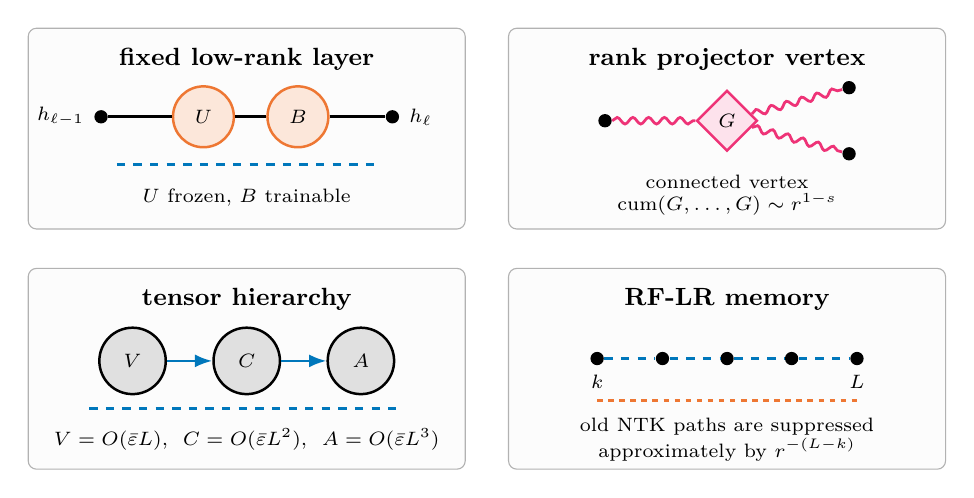
\begin{tikzpicture}[
  x=1cm,
  y=1cm,
  every node/.style={font=\small},
  panel/.style={draw=black!30, rounded corners=3pt, fill=black!1, minimum width=5.55cm, minimum height=2.55cm},
  title/.style={font=\bfseries\small},
  note/.style={font=\scriptsize, align=center},
  sidenote/.style={font=\scriptsize, align=center, text width=2.35cm},
  ext/.style={circle, fill=black, inner sep=1.7pt},
  rankv/.style={circle, draw=color2, fill=color2!18, line width=0.9pt, minimum size=22pt, inner sep=1pt},
  stiefelv/.style={diamond, draw=color4, fill=color4!14, line width=0.9pt, minimum size=22pt, inner sep=1pt},
  tensorv/.style={circle, draw=black, fill=black!12, line width=0.9pt, minimum size=24pt, inner sep=1pt},
  flow/.style={-{Latex[length=2.2mm]}, line width=0.95pt},
  nngp/.style={line width=1pt},
  ntk/.style={color=color1, dash pattern=on 3pt off 3pt, line width=1.1pt},
  rankline/.style={color=color2, dash pattern=on 2pt off 2pt, line width=1.05pt},
  stiefelline/.style={color=color4, decorate, decoration={snake, amplitude=0.42mm, segment length=2mm}, line width=1pt}
]
\node[panel] at (0,0) {};
\node[title] at (0,0.88) {fixed low-rank layer};
\node[ext,label=left:{\scriptsize \(h_{\ell-1}\)}] (h0) at (-1.85,0.15) {};
\node[rankv] (u) at (-0.55,0.15) {\scriptsize \(U\)};
\node[rankv] (b) at (0.65,0.15) {\scriptsize \(B\)};
\node[ext,label=right:{\scriptsize \(h_\ell\)}] (h1) at (1.85,0.15) {};
\draw[nngp] (h0) -- (u) -- (b) -- (h1);
\draw[ntk] (-1.65,-0.46) -- (1.65,-0.46);
\node[note] at (0,-0.87) {\(U\) frozen, \(B\) trainable};

\node[panel] at (6.1,0) {};
\node[title] at (6.1,0.88) {rank projector vertex};
\node[ext] (g1) at (4.55,0.1) {};
\node[stiefelv] (g) at (6.1,0.1) {\scriptsize \(G\)};
\node[ext] (g2) at (7.65,0.52) {};
\node[ext] (g3) at (7.65,-0.32) {};
\draw[stiefelline] (g1) -- (g);
\draw[stiefelline] (g) -- (g2);
\draw[stiefelline] (g) -- (g3);
\node[note] at (6.1,-0.85) {connected vertex\\\(\cumul(G,\ldots,G)\sim r^{1-s}\)};

\node[panel] at (0,-3.05) {};
\node[title] at (0,-2.17) {tensor hierarchy};
\node[tensorv] (V) at (-1.45,-2.95) {\scriptsize \(V\)};
\node[tensorv] (C) at (0,-2.95) {\scriptsize \(C\)};
\node[tensorv] (A) at (1.45,-2.95) {\scriptsize \(A\)};
\draw[flow, color=color1] (V) -- (C);
\draw[flow, color=color1] (C) -- (A);
\draw[ntk] (-2.0,-3.55) -- (2.0,-3.55);
\node[note] at (0,-3.95) {\(V=O(\barE L)\), \(\ C=O(\barE L^2)\), \(\ A=O(\barE L^3)\)};

\node[panel] at (6.1,-3.05) {};
\node[title] at (6.1,-2.17) {RF-LR memory};
\node[ext,label=below:{\scriptsize \(k\)}] (m1) at (4.45,-2.92) {};
\node[ext] (m2) at (5.28,-2.92) {};
\node[ext] (m3) at (6.1,-2.92) {};
\node[ext] (m4) at (6.92,-2.92) {};
\node[ext,label=below:{\scriptsize \(L\)}] (m5) at (7.75,-2.92) {};
\draw[ntk] (m1) -- (m2) -- (m3) -- (m4) -- (m5);
\draw[rankline] (4.45,-3.45) -- (7.75,-3.45);
\node[note] at (6.1,-3.95) {old NTK paths are suppressed\\approximately by \(r^{-(L-k)}\)};
\end{tikzpicture}
}
\caption{Main diagrammatic objects. Solid black lines denote NNGP/preactivation transport, dashed blue lines denote NTK legs, orange vertices denote low-rank factors, pink diamonds denote Stiefel-projector cumulants, and gray blobs denote transported tensor cumulants.}
\label{fig:main-diagrammatic-overview}
\end{figure}

\subsection{Dense NTK rules and low-rank replacement}
\label{app:misof-rule-comparison}
This subsection makes explicit how the finite-width NTK Feynman rules are imported and modified \citep{FeynmanNTK2025}. The dense calculus has the following ingredients.
\begin{enumerate}[leftmargin=1.5em]
\item External filled dots are the observed sample labels. Solid external lines denote preactivation or NNGP objects \(z_\alpha,K_{\alpha\beta}\). Colored dashed external lines denote NTK fluctuations \(\widehat{\Delta\Theta}_{\alpha\beta}\). Double or multi-dashed descendants denote dNTK and ddNTK insertions.
\item Cubic vertices attach two external legs to one internal line. The decoration of the internal line is the local Gaussian-ReLU atom generated by Taylor expansion of the layer map, for example \(\widehat{\Delta\Omega}_{i,\alpha\beta}\), \(\sigma_{i,\alpha}\sigma'_{i,\beta}\), or \(\sigma'_{i,\alpha}\sigma'_{i,\beta}\). In the dense network each such vertex carries the usual \(n_\ell^{-1}\) counting from the neural index.
\item A white propagator is a Gaussian expectation \(\langle\cdot\rangle_{K^{(\ell)}}\). It contracts the decorations of internal lines under the infinite-width NNGP covariance. The selection rules say that propagators connect allowed internal lines, equal neural indices are identified, undecorated dashed NTK lines do not enter the Gaussian expectation, and paired tangent colors contribute the corresponding \(\Theta_{\alpha\beta}^{(\ell)}\) factor.
\item Quartic blobs encode the rank-four tensors that close the order-\(1/n\) dense hierarchy. The \(V\) blob has four \(K\)-legs, \(D,F\) have two \(K\)-legs and two \(\Theta\)-legs, and \(A,B\) have four \(\Theta\)-legs. The same external grammar also defines the higher-derivative tensors \(P,Q,R,S,T,U\) for dNTK and ddNTK.
\item To compute a cumulant or mean correction, one draws all connected diagrams with the prescribed external legs and the desired order in \(1/n\), applies the propagator selection rules, translates each diagram into a Gaussian expectation of derivatives of local atoms, and sums the admissible diagrams.
\end{enumerate}

Our low-rank rules keep this external grammar exactly. The replacement happens only inside the stochastic source:
\[
\scriptstyle
\begin{aligned}
\text{dense neural-index source}
&\longrightarrow
\begin{gathered}[t]
\text{rank-state cumulants } r_\ell^{1-s}\kappa_s^{(\ell)}\\
\text{and projector cumulants }\cumul(G^{(\ell)},\ldots,G^{(\ell)})
\end{gathered}
\\[0.4em]
\frac1{n_\ell}\text{ dense second cumulant}
&\longrightarrow
\frac1{n_\ell}\text{ dense part }
+\gamma_{n_\ell,r_\ell}\text{ projector part }
+\frac1{r_\ell}\text{ rank-state part}.
\end{aligned}
\]
At second order the projector contribution is exactly Lemma \ref{lem:stiefel-cov}. It is proportional to
\[
\gamma_{n,r}=\frac{n(n-r)}{r(n-1)(n+2)},
\]
so it vanishes at \(r=n\). This is the main structural difference from a naive dense replacement \(n\mapsto r\): dense Feynman rules have no reason to cancel at full rank, whereas the isometric low-rank projector rules do.

\subsection{Worked example: one NTK-mean correction}
\label{app:worked-lowrank-diagram}
We now compute one representative diagram in algebraic form. Let \(M_A^{(\ell)}=r_\ell^{-1}\sum_{a=1}^{r_\ell}\phi_A^{(\ell)}(Z_a)\) be a rank-state observable, where \(A\) labels a local atom such as \(\sigma\sigma\), \(\sigma\sigma'\), or \(\sigma'\sigma'\). Suppose the one-layer NTK update can be written locally as a smooth map
\[
\widehat\Theta_{12}^{(\ell+1)}
=\Phi_{12}\!\left(M^{(\ell)},G^{(\ell)}\right)
\text{transported lower-layer terms}.
\]
Taylor expand \(\Phi_{12}\) around the deterministic state \((\bar M,I)\). The connected rank-state part of the mean correction is
\begin{equation}
\E\widehat\Theta_{12}^{(\ell+1)}-\Theta_{12}^{(\ell+1)}
=
\frac{1}{2r_\ell}
\sum_{A,B}
\partial_A\partial_B\Phi_{12}(\bar M,I)\,
\kappa_{AB}^{(\ell)}
+\cdots,
\label{eq:worked-rank-mean}
\end{equation}
where
\[
\kappa_{AB}^{(\ell)}
=\cumul\left(\phi_A^{(\ell)}(Z),\phi_B^{(\ell)}(Z)\right).
\]
This is the low-rank analogue of a Misof propagator diagram: their white Gaussian propagator evaluates a dense neural-index contraction; here the connected empirical-rank vertex evaluates the cumulant of one rank channel and contributes the explicit factor \(r_\ell^{-1}\).

The frozen projector gives a second, full-rank-compatible correction. If \(G=I+\Delta G\), then the leading projector diagram is
\begin{equation}
\begin{aligned}
&\frac12
\sum_{ij,kl}
\partial_{G_{ij}}\partial_{G_{kl}}\Phi_{12}(\bar M,I)\,
\Cov(G_{ij},G_{kl})\\
&\qquad =
\frac{\gamma_{n_\ell,r_\ell}}2
\sum_{ij,kl}
\partial_{G_{ij}}\partial_{G_{kl}}\Phi_{12}(\bar M,I)
\left(\delta_{ik}\delta_{jl}+\delta_{il}\delta_{jk}
-\frac2{n_\ell}\delta_{ij}\delta_{kl}\right).
\end{aligned}
\label{eq:worked-projector-mean}
\end{equation}
Equations \eqref{eq:worked-rank-mean} and \eqref{eq:worked-projector-mean} are the same diagrammatic operation as in the dense NTK calculus: choose the external \(\Theta_{12}\) legs, attach the allowed local vertices, evaluate the connected stochastic source, and sum. The only change is the source value. Dense Misof diagrams count neural-index loops by \(1/n\); our diagrams count rank-channel cumulants by \(1/r\) and Stiefel-projector cumulants by \(\gamma_{n,r}\).

For comparison, the dense next-to-leading NTK mean calculation has five admissible diagrams \citep{FeynmanNTK2025}: transported \(\Theta^{\{1\}}\), transported \(K^{\{1\}}\), and source diagrams from \(V,D,F\). In our notation this becomes the schematic low-rank expansion
\begin{equation}
\Theta^{\{1\}(\ell+1)}_{\mathrm{LR},12}
=
\mathsf T_\Theta[\Theta^{\{1\}(\ell)}_{\mathrm{LR}}]_{12}
\mathsf T_K[K^{\{1\}(\ell)}_{\mathrm{LR}}]_{12}
\mathsf S_V[V_\ell]_{12}
\mathsf S_D[D_\ell]_{12}
\mathsf S_F[F_\ell]_{12},
\label{eq:worked-lowrank-ntk-mean}
\end{equation}
but the tensors \(V,D,F\) now decompose into dense finite-width, rank-state, and projector-defect sources. Thus the external five-diagram grammar is imported unchanged, while the internal weights are changed so that exact full-rank matching is preserved.

\subsection{Summary of the low-rank results encoded by the rules}
\label{app:diagrammatic-results-summary}
The diagrammatic rules above encode the paper's main results as follows.
\begin{enumerate}[leftmargin=1.5em]
\item Exact full-rank matching: when \(r_\ell=n_\ell\), \(U^{(\ell)}\) is orthogonal, \(G=I\), every centered projector vertex vanishes, and the factorized NTK equals the dense NTK pathwise.
\item Stiefel projector covariance: the second projector vertex is \(\Cov(G_{ij},G_{kl})=\gamma_{n,r}(\delta_{ik}\delta_{jl}+\delta_{il}\delta_{jk}-2\delta_{ij}\delta_{kl}/n)\), with \(\gamma_{n,n}=0\).
\item Rank cumulant power counting: a connected \(s\)-point rank-state vertex contributes \(r^{1-s}\). Normalized rank averages therefore have \(s\)-point cumulants of order \(r^{1-s}\).
\item Tensor hierarchy: the imported \(V,C,A\) external grammar remains triangular, with \(V=O(\barE L)\), \(C=O(\barE L^2)\), and \(A=O(\barE L^3)\) under the stated ReLU transport assumptions.
\item Endpoint constants: after pairing-basis extraction, the isolated off-diagonal constants are \(5\) for \(V\), \(21/20\) for the mixed \(C\) sector, and \(173/720\) for the \(A\) sector.
\item Operator criterion: the tensor bounds imply \(\|\widehat\Theta_L-\Theta_{\infty,L}\|_{\op}\lesssim L^{3/2}\sqrt{m\barE}+mL^3\barE\), up to logarithmic factors and the well-spread data condition.
\item RF-LR memory and rank-depth rule: in the bottleneck model, old NTK lines are multiplied by \(\prod_{j=k+1}^L \dot\Sigma^{(j)}/r\), giving geometric memory suppression and the conservative stability rule \(r\gtrsim mL^3\), with the centered/angularized \(mL^2\) rule only under the additional projection hypothesis.
\end{enumerate}

\vspace{-0.8em}
\subsection{Feynman diagram building blocks and tensor assembly}
\label{app:feynman-building-blocks}
The diagrams below should be read as Feynman diagrams, not as decorative notation. A filled dot is an observed sample label. A solid external leg represents a preactivation or NNGP entry \(K_{ab}\). A dashed colored leg represents an NTK fluctuation \(\Delta\Theta_{ab}\). Double or multi-dashed legs represent dNTK and ddNTK descendants. The tensor is determined by the external legs:
\vspace{-0.4em}
\[
\begin{array}{ccl}
K,K &\leadsto& V,\\
K,\Theta &\leadsto& D,F,\\
\Theta,\Theta &\leadsto& A,B,\\
\mathrm d\Theta,K &\leadsto& P,Q,\\
\mathrm{dd}\Theta \text{ external legs} &\leadsto& R,S,T,U.
\end{array}
\]
\vspace{0.2em}
The ordering of sample labels chooses the pairing coordinate. For example, the two \(K\)-leg cumulants \(\cumul(\delta K_{12},\delta K_{34})\), \(\cumul(\delta K_{13},\delta K_{24})\), and \(\cumul(\delta K_{14},\delta K_{23})\) give \(V_{1234}\), \(V_{1324}\), and \(V_{1423}\). Similarly, one solid pair and one dashed pair give \(D_{1234}\), \(F_{1324}\), \(F_{1423}\), while two dashed pairs give \(A_{1234}\), \(B_{1324}\), \(B_{1423}\).

Once the external legs are fixed, every connected diagram is built from the same three operations: transport an older tensor through deterministic \(K\)- or \(\Theta\)-leg derivatives, feed a lower block into a higher block, or attach a fresh low-rank source. The fresh source is where our rules differ from the dense Misof rules: dense neural-index contractions are replaced by rank-state cumulants \(r^{1-s}\kappa_s\) and Stiefel-projector cumulants, whose second-order scale is \(\gamma_{n,r}\).
\iffalse
\begin{figure}[H]
\centering
\resizebox{\linewidth}{!}{%
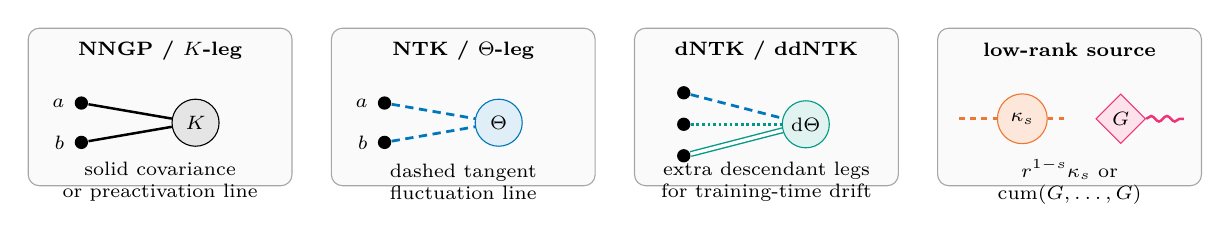
\begin{tikzpicture}[
  x=1cm,
  y=1cm,
  ext/.style={circle, fill=black, inner sep=1.7pt},
  kleg/.style={line width=0.9pt},
  thetaleg/.style={color=color1, dash pattern=on 3pt off 2pt, line width=1pt},
  dleg/.style={color=color6, dash pattern=on 1pt off 1pt, line width=1pt},
  box/.style={draw=black!35, rounded corners, fill=black!2, minimum width=3.35cm, minimum height=2.0cm},
  smalltensor/.style={circle, draw=black, fill=black!10, minimum size=17pt, inner sep=1pt},
  ranklocal/.style={circle, draw=color2, fill=color2!18, minimum size=18pt, inner sep=1pt},
  stiefellocal/.style={diamond, draw=color4, fill=color4!14, minimum size=18pt, inner sep=1pt},
  every node/.style={font=\small}
]
\node[box] at (0,0) {};
\node[font=\bfseries\scriptsize] at (0,0.72) {NNGP / \(K\)-leg};
\node[ext,label=left:{\scriptsize \(a\)}] (k1) at (-1.0,0.05) {};
\node[ext,label=left:{\scriptsize \(b\)}] (k2) at (-1.0,-0.45) {};
\node[smalltensor] (kn) at (0.45,-0.2) {\scriptsize \(K\)};
\draw[kleg] (k1) -- (kn);
\draw[kleg] (k2) -- (kn);
\node[font=\scriptsize, align=center] at (0,-0.95) {solid covariance\\or preactivation line};

\node[box] at (3.85,0) {};
\node[font=\bfseries\scriptsize] at (3.85,0.72) {NTK / \(\Theta\)-leg};
\node[ext,label=left:{\scriptsize \(a\)}] (t1) at (2.85,0.05) {};
\node[ext,label=left:{\scriptsize \(b\)}] (t2) at (2.85,-0.45) {};
\node[smalltensor, draw=color1, fill=color1!12] (tn) at (4.3,-0.2) {\scriptsize \(\Theta\)};
\draw[thetaleg] (t1) -- (tn);
\draw[thetaleg] (t2) -- (tn);
\node[font=\scriptsize, align=center] at (3.85,-0.95) {dashed tangent\\fluctuation line};

\node[box] at (7.7,0) {};
\node[font=\bfseries\scriptsize] at (7.7,0.72) {dNTK / ddNTK};
\node[ext] (d1) at (6.65,0.18) {};
\node[ext] (d2) at (6.65,-0.22) {};
\node[ext] (d3) at (6.65,-0.62) {};
\node[smalltensor, draw=color6, fill=color6!12] (dn) at (8.2,-0.22) {\scriptsize \(\mathrm d\Theta\)};
\draw[thetaleg] (d1) -- (dn);
\draw[dleg] (d2) -- (dn);
\draw[color=color6, double, double distance=1.2pt, line width=0.5pt] (d3) -- (dn);
\node[font=\scriptsize, align=center] at (7.7,-0.95) {extra descendant legs\\for training-time drift};

\node[box] at (11.55,0) {};
\node[font=\bfseries\scriptsize] at (11.55,0.72) {low-rank source};
\node[ranklocal] (rv) at (10.95,-0.15) {\scriptsize \(\kappa_s\)};
\node[stiefellocal] (hv) at (12.2,-0.15) {\scriptsize \(G\)};
\draw[color2, dash pattern=on 2pt off 2pt, line width=1pt] (10.15,-0.15) -- (rv);
\draw[color2, dash pattern=on 2pt off 2pt, line width=1pt] (rv) -- (11.55,-0.15);
\draw[color4, decorate, decoration={snake, amplitude=0.35mm, segment length=2mm}, line width=0.9pt] (hv) -- (13.0,-0.15);
\node[font=\scriptsize, align=center] at (11.55,-0.95) {\(r^{1-s}\kappa_s\) or\\\(\cumul(G,\ldots,G)\)};
\end{tikzpicture}
}
\caption{Feynman diagram building blocks. A \(K\)-leg is a covariance/preactivation external leg, a \(\Theta\)-leg is an NTK fluctuation leg, descendant legs encode dNTK/ddNTK insertions, and the only new low-rank internal vertices are rank cumulants and Stiefel-projector cumulants.}
\label{fig:appendix-visual-dictionary}
\end{figure}
\iffalse
\begin{align}
z_\alpha
&\equiv
\begin{tikzpicture}[baseline=-0.1cm]
  \begin{feynman}
    \vertex[right=0pt, dot, minimum size=3pt, label={left:{\footnotesize \(\alpha\)}}] (x) {};
    \vertex[right=30pt of x, dot, minimum size=0pt] (b) {};
    \diagram*{(x) -- [inner sep=4pt] (b)};
  \end{feynman}
\end{tikzpicture}
\qquad
\widehat{\Delta\Theta}_{\textcolor{color1}{\alpha\beta}}
\equiv
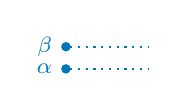
\begin{tikzpicture}[baseline=0.05cm]
  \begin{feynman}
    \vertex[color1, dot, minimum size=3pt, label={left:{\footnotesize \(\textcolor{color1}{\alpha}\)}}] (x1) {};
    \vertex[above=8pt of x1, color1, dot, minimum size=3pt, label={left:{\footnotesize \(\textcolor{color1}{\beta}\)}}] (x2) {};
    \vertex[right=30pt of x1, dot, minimum size=0pt] (b1) {};
    \vertex[right=30pt of x2, dot, minimum size=0pt] (b2) {};
    \diagram*{
      (x1) -- [color1, ghost, inner sep=4pt] (b1),
      (x2) -- [color1, ghost, inner sep=4pt] (b2)
    };
  \end{feynman}
\end{tikzpicture}
\qquad
\widehat{\mathrm d\Theta}
\equiv
\begin{tikzpicture}[baseline=0.05cm]
  \begin{feynman}
    \vertex[color3, dot, minimum size=3pt] (x0) {};
    \vertex[above=8pt of x0, color1, dot, minimum size=3pt] (x1) {};
    \vertex[above=8pt of x1, color6, dot, minimum size=3pt] (x2) {};
    \vertex[right=30pt of x0, dot, minimum size=0pt] (b0) {};
    \vertex[right=30pt of x1, dot, minimum size=0pt] (b1) {};
    \vertex[right=30pt of x2, dot, minimum size=0pt] (b2) {};
    \diagram*{
      (x0) -- [color6color1ddntknew, inner sep=4pt] (b0),
      (x1) -- [color1, ghost, inner sep=4pt] (b1),
      (x2) -- [color6, ghost, inner sep=4pt] (b2)
    };
  \end{feynman}
\end{tikzpicture}.
\label{eq:appendix-visual-external}
\end{align}
The new internal low-rank vertices are:
\begin{align}
\text{rank cumulant}
&\equiv
\begin{tikzpicture}[baseline=(r)]
  \begin{feynman}
    \vertex[rankblob] (r) {\scriptsize \(\kappa_s\)};
    \vertex[left=25pt of r, dot, minimum size=0pt] (l) {};
    \vertex[above right=18pt and 25pt of r, dot, minimum size=0pt] (u) {};
    \vertex[right=25pt of r, dot, minimum size=0pt] (rr) {};
    \vertex[below right=18pt and 25pt of r, dot, minimum size=0pt] (d) {};
    \diagram*{
      (l) -- [color2, ghost] (r),
      (u) -- [color2, ghost] (r),
      (rr) -- [color2, ghost] (r),
      (d) -- [color2, ghost] (r)
    };
  \end{feynman}
\end{tikzpicture}
\sim r^{1-s}\kappa_s,
\qquad
\text{projector cumulant}
\equiv
\begin{tikzpicture}[baseline=(h)]
  \begin{feynman}
    \vertex[stiefelblob] (h) {\scriptsize \(G\)};
    \vertex[left=26pt of h, dot, minimum size=0pt] (l) {};
    \vertex[above right=16pt and 26pt of h, dot, minimum size=0pt] (u) {};
    \vertex[below right=16pt and 26pt of h, dot, minimum size=0pt] (d) {};
    \diagram*{
      (l) -- [color4, photon] (h),
      (u) -- [color4, photon] (h),
      (d) -- [color4, photon] (h)
    };
  \end{feynman}
\end{tikzpicture}
\sim \cumul(G,\ldots,G).
\label{eq:appendix-visual-lowrank}
\end{align}
\fi

\subsection{Rank-state vertices}
Let
\begin{equation}
M_A^{(\ell)}
=\frac1{r_\ell}\sum_{a=1}^{r_\ell}\phi_A^{(\ell)}(Z_a),
\label{eq:appendix-rank-state}
\end{equation}
where \(A\) labels a local atom such as \(\sigma\sigma\), \(\sigma\sigma'\), \(\sigma'\sigma'\), or a derivative analogue. Conditional on the past, the rank atoms are iid. Therefore
\(Z_a\) is the same channel-local random object defined in Lemma \ref{lem:rank-cumulant-counting}, with the layer superscript suppressed.
\begin{equation}
\cumul(M_{A_1}^{(\ell)},\ldots,M_{A_s}^{(\ell)})
=r_\ell^{1-s}\kappa_{A_1\cdots A_s}^{(\ell)},
\qquad
\kappa_{A_1\cdots A_s}^{(\ell)}
=\cumul(\phi_{A_1}^{(\ell)}(Z),\ldots,\phi_{A_s}^{(\ell)}(Z)).
\label{eq:appendix-rank-vertex}
\end{equation}
Thus every connected rank vertex of valence \(s\) has weight \(r_\ell^{1-s}\). In the isometric model, one also has frozen-projector vertices given by cumulants of \(G=(n/r)UU^\top\). At valence two this is Lemma \ref{lem:stiefel-cov}; at higher valence the weights are orthogonal Weingarten contractions. When \(r=n\), \(G=I\), so every centered projector vertex vanishes.

\begin{theorem}[Low-rank Feynman rules]
\label{thm:lowrank-feynman-rules}
Let \(F\) be a smooth observable of finitely many layer states \(M^{(\ell)}\) and frozen projectors \(G^{(\ell)}\). Its expansion in powers of \(1/r_\ell\) and projector cumulants is obtained by summing connected low-rank diagrams with the prescribed external legs. Algebraically:
\begin{enumerate}[leftmargin=1.5em]
\item a rank vertex of valence \(s\) contributes \(r_\ell^{1-s}\kappa_s^{(\ell)}\);
\item a projector vertex contributes the corresponding cumulant of \(G^{(\ell)}\), with second-order scale \(\gamma_{n_\ell,r_\ell}\);
\item a deterministic layer vertex contributes a Frechet derivative \(D^q\Phi_\ell\) of the layer map;
\item a transport edge contributes the product of first derivatives along the depth path;
\item for cumulants, disconnected diagrams cancel by the moment-cumulant relation.
\end{enumerate}
\end{theorem}

\begin{proof}
Taylor expand \(F\) around the deterministic trajectory of the rank states. The cumulant generating operator for an empirical rank average is
\begin{equation}
\exp\left(
\sum_{s\ge2}\frac{r^{1-s}}{s!}
\kappa_{A_1\cdots A_s}
\partial_{A_1}\cdots\partial_{A_s}
\right),
\label{eq:appendix-edgeworth}
\end{equation}
up to the usual finite-order smoothness remainder. Expanding \eqref{eq:appendix-edgeworth} gives the rank vertices and their deterministic derivative contractions. The same argument applies to \(G\), replacing empirical-rank cumulants by frozen-projector cumulants. Taking connected cumulants removes disconnected products.
\end{proof}

\subsection{How large diagrams reduce to the formulas}
\label{app:diagram-reduction}
The diagrams are not only notation for the vertices; they are a bookkeeping device for reducing a large Taylor-cumulant expansion to the compact recursions used in the main text. A diagram has three kinds of pieces. External legs are sample-pair observables such as \(K_{12}\), \(K_{34}\), \(\Theta_{12}\), and \(\Theta_{34}\). Deterministic layer boxes are derivatives of the infinite-width layer map, and they transport external legs from layer \(\ell\) to layer \(\ell+1\). Rank or projector blobs are the only random connected sources; they insert either \(r^{1-s}\kappa_s\) or a Stiefel-projector cumulant, whose second-order size is \(\gamma_{n,r}\).

The reduction rule is the following. First fix the external observable, for example
\[
\cumul(\delta\Theta^{(\ell+1)}_{12},\delta\Theta^{(\ell+1)}_{34}).
\]
Then Taylor expand each \(\Theta^{(\ell+1)}\) in the previous layer variables \(K^{(\ell)}\), \(\Theta^{(\ell)}\), and the new rank/projector atoms. Each term becomes a diagram. If a diagram disconnects after removing the external labels, it cancels in the connected cumulant. If it stays connected, all internal sample indices are contracted by the Kronecker deltas from Gaussian-ReLU derivatives and Stiefel cumulants. The remaining expression is a deterministic derivative coefficient multiplying one lower-layer tensor or one new source.

\begin{figure}[H]
\centering
\resizebox{\linewidth}{!}{%
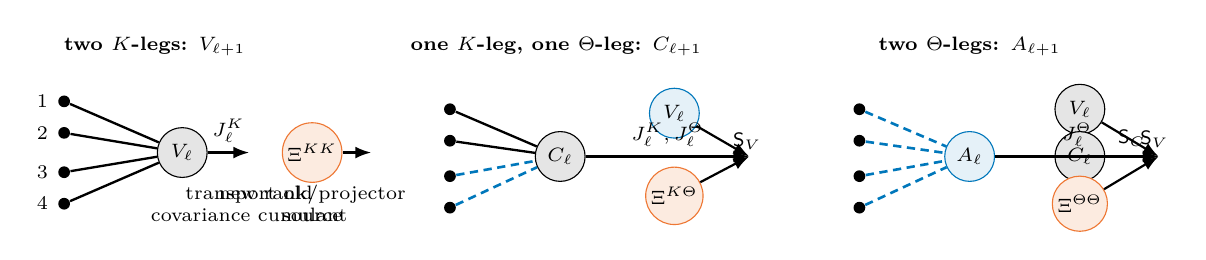
\begin{tikzpicture}[
  x=1cm,
  y=1cm,
  ext/.style={circle, fill=black, inner sep=1.5pt},
  kleg/.style={line width=0.85pt},
  thetaleg/.style={color=color1, dash pattern=on 3pt off 2pt, line width=0.95pt},
  flow/.style={-{Latex[length=2mm]}, line width=0.8pt},
  tensor/.style={circle, draw=black, fill=black!10, minimum size=18pt, inner sep=1pt},
  source/.style={circle, draw=color2, fill=color2!15, minimum size=18pt, inner sep=1pt},
  proj/.style={diamond, draw=color4, fill=color4!12, minimum size=18pt, inner sep=1pt},
  every node/.style={font=\small}
]
\node[font=\bfseries\scriptsize] at (0,1.15) {two \(K\)-legs: \(V_{\ell+1}\)};
\node[ext,label=left:{\scriptsize \(1\)}] (v1) at (-1.15,0.45) {};
\node[ext,label=left:{\scriptsize \(2\)}] (v2) at (-1.15,0.05) {};
\node[ext,label=left:{\scriptsize \(3\)}] (v3) at (-1.15,-0.45) {};
\node[ext,label=left:{\scriptsize \(4\)}] (v4) at (-1.15,-0.85) {};
\node[tensor] (Vold) at (0.35,-0.2) {\scriptsize \(V_\ell\)};
\draw[kleg] (v1) -- (Vold);
\draw[kleg] (v2) -- (Vold);
\draw[kleg] (v3) -- (Vold);
\draw[kleg] (v4) -- (Vold);
\node[source] (Vsrc) at (2.0,-0.2) {\scriptsize \(\Xi^{KK}\)};
\draw[flow] (Vold) -- node[above,font=\scriptsize] {\(J^K_\ell\)} (1.2,-0.2);
\node[font=\scriptsize, align=center] at (1.2,-0.85) {transport old\\covariance cumulant};
\draw[flow] (Vsrc) -- (2.75,-0.2);
\node[font=\scriptsize, align=center] at (2.0,-0.85) {new rank/projector\\source};

\node[font=\bfseries\scriptsize] at (5.1,1.15) {one \(K\)-leg, one \(\Theta\)-leg: \(C_{\ell+1}\)};
\node[ext] (c1) at (3.75,0.35) {};
\node[ext] (c2) at (3.75,-0.05) {};
\node[ext] (c3) at (3.75,-0.5) {};
\node[ext] (c4) at (3.75,-0.9) {};
\node[tensor] (Cold) at (5.15,-0.25) {\scriptsize \(C_\ell\)};
\draw[kleg] (c1) -- (Cold);
\draw[kleg] (c2) -- (Cold);
\draw[thetaleg] (c3) -- (Cold);
\draw[thetaleg] (c4) -- (Cold);
\node[tensor, draw=color1, fill=color1!10] (Cfeed) at (6.6,0.3) {\scriptsize \(V_\ell\)};
\node[source] (Csrc) at (6.6,-0.75) {\scriptsize \(\Xi^{K\Theta}\)};
\draw[flow] (Cold) -- node[above,font=\scriptsize] {\(J^K_\ell,J^\Theta_\ell\)} (7.55,-0.25);
\draw[flow] (Cfeed) -- node[right,font=\scriptsize] {\(\mathsf S_V\)} (7.55,-0.25);
\draw[flow] (Csrc) -- (7.55,-0.25);

\node[font=\bfseries\scriptsize] at (10.35,1.15) {two \(\Theta\)-legs: \(A_{\ell+1}\)};
\node[ext] (a1) at (8.95,0.35) {};
\node[ext] (a2) at (8.95,-0.05) {};
\node[ext] (a3) at (8.95,-0.5) {};
\node[ext] (a4) at (8.95,-0.9) {};
\node[tensor, draw=color1, fill=color1!10] (Aold) at (10.35,-0.25) {\scriptsize \(A_\ell\)};
\draw[thetaleg] (a1) -- (Aold);
\draw[thetaleg] (a2) -- (Aold);
\draw[thetaleg] (a3) -- (Aold);
\draw[thetaleg] (a4) -- (Aold);
\node[tensor] (AfeedV) at (11.75,0.35) {\scriptsize \(V_\ell\)};
\node[tensor] (AfeedC) at (11.75,-0.25) {\scriptsize \(C_\ell\)};
\node[source] (Asrc) at (11.75,-0.85) {\scriptsize \(\Xi^{\Theta\Theta}\)};
\draw[flow] (Aold) -- node[above,font=\scriptsize] {\(J^\Theta_\ell\)} (12.75,-0.25);
\draw[flow] (AfeedV) -- node[right,font=\scriptsize] {\(\mathsf S_V\)} (12.75,-0.25);
\draw[flow] (AfeedC) -- node[above,font=\scriptsize] {\(\mathsf S_C\)} (12.75,-0.25);
\draw[flow] (Asrc) -- (12.75,-0.25);
\end{tikzpicture}
}
\caption{Diagrammatic reduction of the tensor hierarchy. The external legs decide which block is being computed: two \(K\)-legs give \(V\), one \(K\)-leg and one \(\Theta\)-leg give \(C=(D,F)\), and two \(\Theta\)-legs give \(A=(A,B)\). After Taylor expansion, connected diagrams either transport an older tensor through deterministic derivatives \(J^K_\ell,J^\Theta_\ell\), feed lower blocks through \(\mathsf S_V,\mathsf S_C\), or create a fresh low-rank source \(\Xi\).}
\label{fig:appendix-diagram-reduction-disabled}
\end{figure}
\fi

\begin{figure}[H]
\centering
\resizebox{\linewidth}{!}{%
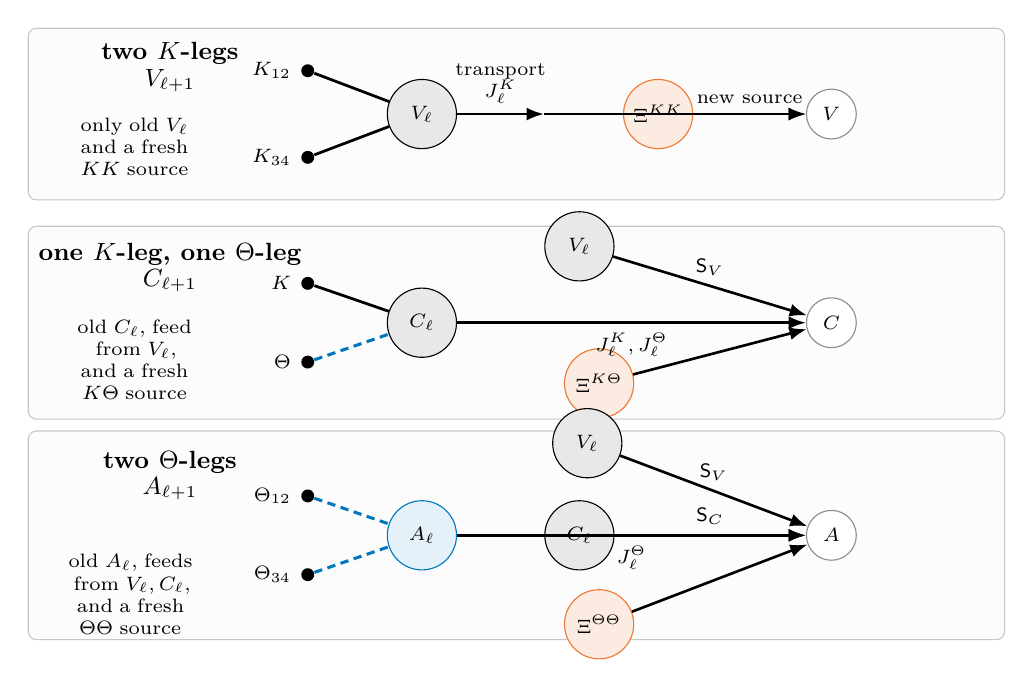
\begin{tikzpicture}[
  x=1cm,
  y=1cm,
  ext/.style={circle, fill=black, inner sep=1.65pt},
  kleg/.style={line width=1pt},
  thetaleg/.style={color=color1, dash pattern=on 3pt off 2pt, line width=1.1pt},
  flow/.style={-{Latex[length=2.2mm]}, line width=0.95pt},
  tensor/.style={circle, draw=black, fill=black!9, minimum size=25pt, inner sep=1pt},
  source/.style={circle, draw=color2, fill=color2!15, minimum size=25pt, inner sep=1pt},
  outnode/.style={circle, draw=black!45, fill=white, minimum size=18pt, inner sep=0.5pt},
  panel/.style={draw=black!22, rounded corners=3pt, fill=black!1, minimum width=12.4cm, minimum height=2.18cm},
  title/.style={font=\bfseries\small},
  note/.style={font=\scriptsize, align=center},
  sidenote/.style={font=\scriptsize, align=center, text width=2.35cm},
  every node/.style={font=\small}
]
\node[panel] at (0,0) {};
\node[title] at (-4.4,0.77) {two \(K\)-legs};
\node[title] at (-4.4,0.43) {\(V_{\ell+1}\)};
\node[sidenote] at (-4.85,-0.42) {only old \(V_\ell\)\\and a fresh \(KK\) source};
\node[ext,label=left:{\scriptsize \(K_{12}\)}] (v1) at (-2.65,0.55) {};
\node[ext,label=left:{\scriptsize \(K_{34}\)}] (v2) at (-2.65,-0.55) {};
\node[tensor] (Vold) at (-1.2,0.0) {\scriptsize \(V_\ell\)};
\node[source] (Vsrc) at (1.8,0.0) {\scriptsize \(\Xi^{KK}\)};
\node[outnode] (Vout) at (4.0,0.0) {\scriptsize \(V\)};
\draw[kleg] (v1) -- (Vold);
\draw[kleg] (v2) -- (Vold);
\draw[flow] (Vold) -- node[above,note] {transport\\\(J^K_\ell\)} (0.35,0.0);
\draw[flow] (0.35,0.0) -- (Vout);
\draw[flow] (Vsrc) -- node[above,note] {new source} (Vout);

\node[panel, minimum height=2.45cm] at (0,-2.65) {};
\node[title] at (-4.4,-1.78) {one \(K\)-leg, one \(\Theta\)-leg};
\node[title] at (-4.4,-2.12) {\(C_{\ell+1}\)};
\node[sidenote] at (-4.85,-3.12) {old \(C_\ell\), feed from \(V_\ell\),\\and a fresh \(K\Theta\) source};
\node[ext,label=left:{\scriptsize \(K\)}] (c1) at (-2.65,-2.15) {};
\node[ext,label=left:{\scriptsize \(\Theta\)}] (c2) at (-2.65,-3.15) {};
\node[tensor] (Cold) at (-1.2,-2.65) {\scriptsize \(C_\ell\)};
\node[tensor] (Cfeed) at (0.8,-1.68) {\scriptsize \(V_\ell\)};
\node[source] (Csrc) at (1.05,-3.42) {\scriptsize \(\Xi^{K\Theta}\)};
\node[outnode] (Cout) at (4.0,-2.65) {\scriptsize \(C\)};
\draw[kleg] (c1) -- (Cold);
\draw[thetaleg] (c2) -- (Cold);
\draw[flow] (Cold) -- node[below,note] {\(J^K_\ell,J^\Theta_\ell\)} (Cout);
\draw[flow] (Cfeed) -- node[above,note] {\(\mathsf S_V\)} (Cout);
\draw[flow] (Csrc) -- (Cout);

\node[panel, minimum height=2.65cm] at (0,-5.35) {};
\node[title] at (-4.4,-4.42) {two \(\Theta\)-legs};
\node[title] at (-4.4,-4.76) {\(A_{\ell+1}\)};
\node[sidenote] at (-4.9,-6.10) {old \(A_\ell\), feeds from \(V_\ell,C_\ell\),\\and a fresh \(\Theta\Theta\) source};
\node[ext,label=left:{\scriptsize \(\Theta_{12}\)}] (a1) at (-2.65,-4.85) {};
\node[ext,label=left:{\scriptsize \(\Theta_{34}\)}] (a2) at (-2.65,-5.85) {};
\node[tensor, draw=color1, fill=color1!10] (Aold) at (-1.2,-5.35) {\scriptsize \(A_\ell\)};
\node[tensor] (AfeedV) at (0.9,-4.18) {\scriptsize \(V_\ell\)};
\node[tensor] (AfeedC) at (0.8,-5.35) {\scriptsize \(C_\ell\)};
\node[source] (Asrc) at (1.05,-6.48) {\scriptsize \(\Xi^{\Theta\Theta}\)};
\node[outnode] (Aout) at (4.0,-5.35) {\scriptsize \(A\)};
\draw[thetaleg] (a1) -- (Aold);
\draw[thetaleg] (a2) -- (Aold);
\draw[flow] (Aold) -- node[below,note] {\(J^\Theta_\ell\)} (Aout);
\draw[flow] (AfeedV) -- node[above,note] {\(\mathsf S_V\)} (Aout);
\draw[flow] (AfeedC) -- node[above,note] {\(\mathsf S_C\)} (Aout);
\draw[flow] (Asrc) -- (Aout);
\end{tikzpicture}
}
\caption{Diagrammatic reduction of the tensor hierarchy. External \(K\)- and \(\Theta\)-legs choose the block being computed. Connected terms either transport an older tensor, feed a lower block into a higher one, or create a fresh low-rank source \(\Xi\).}
\label{fig:appendix-diagram-reduction}
\end{figure}

For the NTK-NTK block this gives the schematic reduction
\begin{equation}
\begin{aligned}
\cumul(\delta\Theta^{(\ell+1)}_{12},\delta\Theta^{(\ell+1)}_{34})
&=
\underbrace{J^\Theta_\ell
\cumul(\delta\Theta^{(\ell)}_{12},\delta\Theta^{(\ell)}_{34})
(J^\Theta_\ell)^\top}_{\text{transported old NTK-NTK diagram}}\\
&\quad+
\underbrace{\mathsf S_C[C_\ell]+\mathsf S_V[V_\ell]}_{\text{mixed diagrams feeding into NTK-NTK}}+
\underbrace{\Xi^{\Theta\Theta}_\ell}_{\text{new connected rank/projector source}}.
\end{aligned}
\label{eq:appendix-diagram-reduction-A}
\end{equation}
The same operation with two \(K\)-legs gives \(V_{\ell+1}\), and with one \(K\)-leg and one \(\Theta\)-leg gives \(C_{\ell+1}\). Thus the apparently large expansion collapses because every connected diagram has only two possible roles: it either transports an older tensor through \(J^K_\ell\) or \(J^\Theta_\ell\), or it creates a fresh source \(\Xi\). This is the mechanism behind the triangular recursion in \eqref{eq:tensor-triangular-recursion}.

\subsection{Basic tensor recursions}
The diagrammatic rules produce the same external tensor hierarchy as the dense finite-width expansion, but with low-rank sources. Let \(J^K_\ell\) and \(J^\Theta_\ell\) denote the deterministic linear transports for NNGP and NTK legs. The NNGP covariance block satisfies schematically
\begin{equation}
V_{\ell+1}
=J^K_\ell V_\ell (J^K_\ell)^\top+\Xi^{KK}_\ell,
\qquad
\Xi^{KK}_\ell
=r_\ell^{-1}\kappa_2(S^K,S^K)
+\gamma_{n_\ell,r_\ell}\mathfrak h^{KK}_\ell.
\label{eq:appendix-V-rec}
\end{equation}
For the mixed NNGP-NTK block \(C=(D,F)\),
\begin{equation}
C_{\ell+1}
=J^K_\ell C_\ell (J^\Theta_\ell)^\top
+\mathsf S_V[V_\ell]
+\Xi^{K\Theta}_\ell.
\label{eq:appendix-C-rec}
\end{equation}
For the NTK-NTK block \(A=(A,B)\),
\begin{equation}
A_{\ell+1}
=J^\Theta_\ell A_\ell (J^\Theta_\ell)^\top
+\mathsf S_C[C_\ell]+\mathsf S_V[V_\ell]
+\Xi^{\Theta\Theta}_\ell.
\label{eq:appendix-A-rec}
\end{equation}
The sources \(\Xi^{KK}\), \(\Xi^{K\Theta}\), and \(\Xi^{\Theta\Theta}\) are precisely the rank and projector cumulant vertices with the corresponding external legs. The next display should be read only as a source dictionary. It is not a separate calculation: it says which connected second cumulant is injected into each tensor block. The rank/projector blob labelled \(\kappa_2\) contributes the small factor \(r^{-1}\), \(1/n\), or \(\gamma_{n,r}\). The number of external \(\Theta\)-legs then determines how many NTK transports are accumulated over depth, and therefore whether the block grows like \(L\), \(L^2\), or \(L^3\).
\begin{equation}
\begin{tikzpicture}[baseline=(vbase)]
  \begin{feynman}
    \vertex (vbase) at (0,0) {};
    \vertex[dot, minimum size=3pt] (k1) at (0,0.45) {};
    \vertex[dot, minimum size=3pt] (k2) at (0,-0.45) {};
    \vertex[quarticblob] (v) at (1.6,0) {\scriptsize \(V\)};
    \vertex[rankblob] (rv) at (3.3,0) {\scriptsize \(\kappa_2\)};
    \diagram*{
      (k1) -- (v) -- (k2),
      (v) -- [color2, ghost, edge label={\scriptsize source}] (rv)
    };
  \end{feynman}
\end{tikzpicture}
\qquad
\begin{tikzpicture}[baseline=(cbase)]
  \begin{feynman}
    \vertex (cbase) at (0,0) {};
    \vertex[dot, minimum size=3pt] (k) at (0,0.45) {};
    \vertex[color1, dot, minimum size=3pt] (t) at (0,-0.45) {};
    \vertex[quarticblob] (c) at (1.6,0) {\scriptsize \(C\)};
    \vertex[rankblob] (rc) at (3.3,0) {\scriptsize \(\kappa_2\)};
    \diagram*{
      (k) -- (c),
      (t) -- [color1, ghost] (c),
      (c) -- [color2, ghost, edge label={\scriptsize source}] (rc)
    };
  \end{feynman}
\end{tikzpicture}
\qquad
\begin{tikzpicture}[baseline=(abase)]
  \begin{feynman}
    \vertex (abase) at (0,0) {};
    \vertex[color1, dot, minimum size=3pt] (t1) at (0,0.45) {};
    \vertex[color2, dot, minimum size=3pt] (t2) at (0,-0.45) {};
    \vertex[quarticblob] (a) at (1.6,0) {\scriptsize \(A\)};
    \vertex[rankblob] (ra) at (3.3,0) {\scriptsize \(\kappa_2\)};
    \diagram*{
      (t1) -- [color1, ghost] (a),
      (t2) -- [color2, ghost] (a),
      (a) -- [color2, ghost, edge label={\scriptsize source}] (ra)
    };
  \end{feynman}
\end{tikzpicture}
\label{eq:appendix-visual-VCA}
\end{equation}
Equivalently, the diagrammatic message is
\begin{center}
\small
\begin{tabular}{lllp{0.42\linewidth}}
\toprule
External legs & Tensor block & Fresh source size & Depth accumulation \\
\midrule
\(K,K\) & \(V=\cumul(K,K)\) & \(O(\barE)\) & no transported NTK leg, hence \(O(\barE L)\) \\
\(K,\Theta\) & \(C=(D,F)\) & \(O(\barE)\) & one transported NTK leg, hence \(O(\barE L^2)\) \\
\(\Theta,\Theta\) & \(A=(A,B)\) & \(O(\barE)\) & two transported NTK legs, hence \(O(\barE L^3)\) \\
\bottomrule
\end{tabular}
\end{center}
Thus the diagrams separate two effects that are easy to confuse. The orange/rank blob gives the perturbative smallness; it does not decide the power of \(L\). The external \(K\)- and \(\Theta\)-legs decide the depth power through deterministic transport.

\subsection{First NTK mean correction}
The familiar finite-width correction to the NTK mean has the same external five-term form:
\begin{equation}
\Theta^{\{1\}}_{\ell+1}
=\mathsf T_\Theta[\Theta^{\{1\}}_\ell]
+\mathsf T_K[K^{\{1\}}_\ell]
+\mathsf S_V[V_\ell]
+\mathsf S_D[D_\ell]
+\mathsf S_F[F_\ell].
\label{eq:appendix-theta-five}
\end{equation}
The low-rank difference is that the source tensors \(V,D,F\) are further resolved into the rank-state and projector vertices above. Thus the low-rank calculus does not change the external NTK grammar; it changes the internal expansion parameter from neural-index contractions to empirical-rank cumulants and frozen-projector cumulants.

\subsection{Full tensor dictionary}
\label{app:full-tensor-dictionary}
For four sample labels \(1,2,3,4\), write
\[
\delta K_{ab}^{(\ell)}:=K_{ab}^{(\ell)}-\E K_{ab}^{(\ell)},
\qquad
\delta\Theta_{ab}^{(\ell)}:=\Theta_{ab}^{(\ell)}-\E\Theta_{ab}^{(\ell)}.
\]
All coordinates below are centered two-point cumulants of these pair observables. Since the variables are centered, \(\cumul(X,Y)=\E[XY]\). In particular, \(V_{1234}^{(\ell)}=\E[\delta K_{12}^{(\ell)}\delta K_{34}^{(\ell)}]\), \(D_{1234}^{(\ell)}=\E[\delta K_{12}^{(\ell)}\delta\Theta_{34}^{(\ell)}]\), \(F_{1324}^{(\ell)}=\E[\delta K_{13}^{(\ell)}\delta\Theta_{24}^{(\ell)}]\), \(A_{1234}^{(\ell)}=\E[\delta\Theta_{12}^{(\ell)}\delta\Theta_{34}^{(\ell)}]\), and \(B_{1324}^{(\ell)}=\E[\delta\Theta_{13}^{(\ell)}\delta\Theta_{24}^{(\ell)}]\). The rank-four tensor basis is organized by the three pairings \((12|34)\), \((13|24)\), and \((14|23)\). The NNGP-NNGP block is
\begin{align}
\mathcal V_\ell
&=
\begin{pmatrix}
V_{1234}^{(\ell)}\\
V_{1324}^{(\ell)}\\
V_{1423}^{(\ell)}
\end{pmatrix}
:=
\begin{pmatrix}
\cumul(\delta K_{12}^{(\ell)},\delta K_{34}^{(\ell)})\\
\cumul(\delta K_{13}^{(\ell)},\delta K_{24}^{(\ell)})\\
\cumul(\delta K_{14}^{(\ell)},\delta K_{23}^{(\ell)})
\end{pmatrix}.
\label{eq:V-full-dictionary}
\end{align}
The mixed NNGP-NTK block is
\begin{align}
\mathcal C_\ell
&=
\begin{pmatrix}
D_{1234}^{(\ell)}\\
F_{1324}^{(\ell)}\\
F_{1423}^{(\ell)}
\end{pmatrix}
:=
\begin{pmatrix}
\cumul(\delta K_{12}^{(\ell)},\delta\Theta_{34}^{(\ell)})\\
\cumul(\delta K_{13}^{(\ell)},\delta\Theta_{24}^{(\ell)})\\
\cumul(\delta K_{14}^{(\ell)},\delta\Theta_{23}^{(\ell)})
\end{pmatrix}.
\label{eq:C-full-dictionary}
\end{align}
The NTK-NTK block is
\begin{align}
\mathcal A_\ell
&=
\begin{pmatrix}
A_{1234}^{(\ell)}\\
B_{1324}^{(\ell)}\\
B_{1423}^{(\ell)}
\end{pmatrix}
:=
\begin{pmatrix}
\cumul(\delta\Theta_{12}^{(\ell)},\delta\Theta_{34}^{(\ell)})\\
\cumul(\delta\Theta_{13}^{(\ell)},\delta\Theta_{24}^{(\ell)})\\
\cumul(\delta\Theta_{14}^{(\ell)},\delta\Theta_{23}^{(\ell)})
\end{pmatrix}.
\label{eq:A-full-dictionary}
\end{align}
This is the tensor dictionary behind the compact \(V,C,A\) notation in the main text: \(C=(D,F)\) and \(A=(A,B)\). The dense finite-width Feynman sectors remain the same, but their low-rank stochastic vertices are cumulants of the frozen projector \(G=(n/r)UU^\top\).

\subsection{Pairing extraction}
A rank-four orthogonally invariant tensor decomposes as
\begin{equation}
C_{i_1i_2i_3i_4}
=c_1\delta_{i_1i_2}\delta_{i_3i_4}
+c_2\delta_{i_1i_3}\delta_{i_2i_4}
+c_3\delta_{i_1i_4}\delta_{i_2i_3}.
\label{eq:appendix-pairing}
\end{equation}
Let \(B_1,B_2,B_3\) be the three pairings. The normalized pairing Gram matrix is
\begin{equation}
\overline G_N
=
\begin{pmatrix}
1&1/N&1/N\\
1/N&1&1/N\\
1/N&1/N&1
\end{pmatrix},
\qquad
\overline G_N^{-1}
=\frac{N}{N-1}I_3-\frac{N}{(N-1)(N+2)}\one\one^\top.
\label{eq:appendix-pairing-inv}
\end{equation}
If \(h=(\langle C,B_1\rangle,\langle C,B_2\rangle,\langle C,B_3\rangle)\) are measured contractions, the isolated tensor coefficients are \((c_1,c_2,c_3)^\top=\overline G_N^{-1}h\). This is why direct scalar-output cumulants should not be identified with the endpoint coefficients \(5\), \(21/20\), and \(173/720\) without a pairing-basis extraction.

\subsection{Centered RF-LR memory lemma}
For RF-LR, an old NTK line transported from layer \(k\) to \(L\) carries
\begin{equation}
B_{L:k}
=\prod_{s=k+1}^{L}\frac1r\dot\Sigma^{(s)}.
\label{eq:appendix-rflr-product}
\end{equation}
At ReLU edge of chaos, \(\dot\Sigma^{(s)}\to1/2\), so \(\|B_{L:k}\|\lesssim (2r)^{-(L-k)}\), up to polynomial endpoint factors. The corresponding centered transport diagram is
\begin{equation}
\begin{tikzpicture}[baseline=(y)]
  \begin{feynman}
    \vertex[projblob] (p1) at (0,0) {\scriptsize \(P\)};
    \vertex[rankblob] (y) at (1.1,0) {\scriptsize \(Y_k\)};
    \vertex[smallblob] (b1) at (2.3,0) {};
    \vertex (dots) at (3.0,0) {\(\cdots\)};
    \vertex[smallblob] (b2) at (3.8,0) {};
    \vertex[projblob] (p2) at (5.0,0) {\scriptsize \(P\)};
    \diagram*{
      (p1) -- [color1, ghost] (y) -- [color1, ghost, edge label={\scriptsize \(b\simeq(2r)^{-1}\)}] (b1),
      (b2) -- [color1, ghost] (p2)
    };
    \draw[color1,dash pattern=on 3pt off 3pt,line width=1pt] (b1) -- (dots);
    \draw[color1,dash pattern=on 3pt off 3pt,line width=1pt] (dots) -- (b2);
  \end{feynman}
\end{tikzpicture}
\label{eq:appendix-visual-centered-memory}
\end{equation}
Let \(P=I-\one\one^\top/m\) and \(Z_L=P(\widehat K_L-K_L)P\). The centered fluctuation admits the linearized expansion
\begin{equation}
Z_L
=\sum_{k=1}^{L}B_{L:k+1}Y_k
+\sum_{k=1}^{L}B_{L:k+1}R_k,
\label{eq:appendix-centered-expansion}
\end{equation}
where \(Y_k\) is a centered fresh rank source and \(R_k\) is quadratic in earlier fluctuations.

\begin{lemma}[Centered RF-LR memory]
\label{lem:centered-rflr-memory}
Assume, conditionally on the past,
\begin{equation}
\left\|\E[Y_k^2\mid\mathcal F_{k-1}]\right\|_{\op}
\le C\frac{m\eps_{\RF}}{r^2},
\qquad
\|Y_k\|_{\psi_1}\le C\frac{\sqrt{\eps_{\RF}}}{r},
\label{eq:appendix-Y-bound}
\end{equation}
and \(\|B_{L:k}\|\le q^{L-k}\) for some \(q<1\). If \(\|R_k\|_{\op}\le C m\eps_{\RF}/r^2\) with high probability, then, up to logarithmic factors,
\begin{equation}
\|Z_L\|_{\op}
\lesssim
\frac{\sqrt{m\eps_{\RF}\log(m/\delta)}}{r}
+
\frac{m\eps_{\RF}\log(m/\delta)}{r^2}
\label{eq:appendix-centered-lemma}
\end{equation}
with probability at least \(1-\delta\).
\end{lemma}

\begin{proof}
Set \(X_k=B_{L:k+1}Y_k\). The predictable matrix variance satisfies
\begin{equation}
\left\|\sum_{k=1}^{L}\E[X_k^2\mid\mathcal F_{k-1}]\right\|_{\op}
\le
C\frac{m\eps_{\RF}}{r^2}\sum_{k=1}^{L}q^{2(L-k)}
\le C'\frac{m\eps_{\RF}}{r^2}.
\end{equation}
Matrix Freedman or Bernstein gives the first term in \eqref{eq:appendix-centered-lemma}. For the quadratic remainder,
\begin{equation}
\left\|\sum_{k=1}^{L}B_{L:k+1}R_k\right\|_{\op}
\le
C\frac{m\eps_{\RF}}{r^2}\sum_{k=1}^{L}q^{L-k}
\le C'\frac{m\eps_{\RF}}{r^2}.
\end{equation}
\end{proof}

Combining Lemma \ref{lem:centered-rflr-memory} with Weyl's inequality gives the centered/angularized criterion. If the centered deterministic margin satisfies \(\lambda_{\min}(PK_LP)\gtrsim (rL)^{-1}\), and if \(\eps_{\RF}\simeq 1/r\), then the fluctuation bound is below the margin when
\begin{equation}
r\gtrsim mL^2
\label{eq:appendix-centered-L2}
\end{equation}
up to logarithms. Without removing the radial constant mode, a diffusive \(\sqrt L\) factor can reappear, giving the conservative cubic-depth criterion used for the unprojected RF-LR statement.

\section{Extended True Finite-Network Experiments}
\label{app:extended-experiments}
This appendix keeps the detailed diagnostics out of the main ten-page narrative while preserving the evidence used to interpret the finite-network checks.

\subsection{Experimental methodology}
All true finite-network experiments use scalar-output ReLU networks with the signed/isometric factorization \(W^{(\ell)}=\sigma_w n_{\ell-1}^{-1/2}\sqrt{n_\ell/r_\ell}\,U^{(\ell)}B^{(\ell)}\). The left factors \(U^{(\ell)}\) are sampled uniformly from the Stiefel manifold and held fixed; the empirical NTK is computed by PyTorch autograd with respect to the trainable right factors \(B^{(\ell)}\) and the readout. Inputs are synthetic, fixed across the compared initializations, and normalized to unit Euclidean norm. The reported quantities are not training accuracies: they are initialization-time NTK and NNGP diagnostics designed to test the rank-width perturbation theory.

For the clean true-NTK operator and rank-defect sweep, we use width \(n=128\), sample size \(m=8\), input dimension \(d=16\), ranks \(r\in\{8,16,32,64,128\}\), and depths \(L\in\{2,3,4,5,6,8,10\}\). For each pair \((r,L)\), 200 independent initializations are drawn. For a fixed \((r,L)\), we compute the empirical NTK Gram matrix \(\widehat\Theta\), subtract its initialization mean across seeds, and report the median and mean operator norm of the fluctuation. The normalization in Figure \ref{fig:true-ntk-operator-rank} is \(L^{3/2}\sqrt{m\varepsilon}\), with \(\varepsilon=1/n+\gamma_{n,r}\). The rank-defect panel fixes the largest depth in this sweep and varies \(r\), checking that the excess low-rank contribution follows the defect scale and disappears at \(r=n\). Exact full-rank matching is tested separately at \(n=r=128\), \(m=8\), \(d=16\), and depths up to \(L=200\); because the theorem is pathwise, this test measures numerical precision rather than a statistical average.

For direct finite-network cumulants, we again use \(n=128\), \(m=8\), \(d=16\), and ranks \(r\in\{8,16,32,64,128\}\). For every \((r,L)\), 2000 independent initializations are used. The standard long sweep uses depths \(L\in\{2,3,4,5,6,8,10,12,14,16,20\}\). The deep stress test uses \(L\in\{20,50,100,200\}\). For each initialization we compute the final hidden-feature Gram matrix \(K=h_Lh_L^\top/n\) and the empirical NTK \(\Theta=JJ^\top\). Across seeds we estimate the centered second cumulants \(V=\cumul(K,K)\), \(C=\cumul(K,\Theta)\), and \(A=\cumul(\Theta,\Theta)\) on fixed same-off-diagonal and disjoint-off-diagonal sample pairings. The log-log slopes in Table \ref{tab:effective-cumulant-slopes} are ordinary least-squares fits of \(\log|\text{cumulant}|\) against \(\log L\) over the listed depth set for each rank. These slopes are diagnostic effective exponents of contracted scalar-output observables; they are not estimates of isolated pairing-basis tensor constants.

The proxy experiments in the main text are separate Monte Carlo checks of closed-form quantities. The Stiefel-projector covariance experiment uses \(n=64\), ranks \(r\in\{4,8,16,32,64\}\), and 50,000 Stiefel samples to compare \(\Cov(G_{12},G_{12})\) with \(\gamma_{n,r}\). The scalar endpoint-constant experiment uses \(\varepsilon=10^{-3}\), depths \(L\in\{8,12,16,24,32,48,64,96,128,192,256\}\), and 200,000 Monte Carlo samples to check convergence of the normalized \(V\), \(C\), and \(A\) proxies to \(5\), \(21/20\), and \(173/720\). The operator proxy uses \(m=64\) and 300 repetitions per depth to check stability of the normalization \(L^{3/2}\sqrt{m\varepsilon}\). The RF-LR memory panel uses ranks \(2,4,8,16\) and tracks the product of old-NTK transport factors over ages up to 24 layers.

\begin{figure}[H]
\centering
\begin{minipage}{0.43\linewidth}
\centering
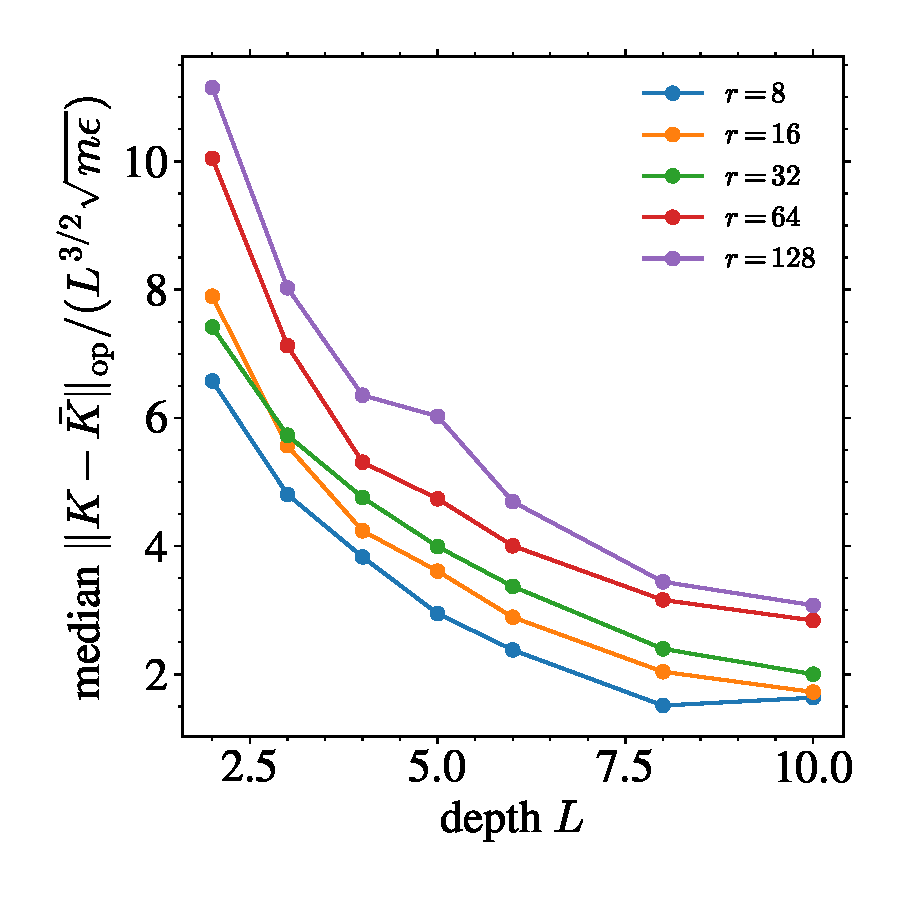
\includegraphics[width=0.92\linewidth]{../../data/feynman/true_finite_ntk_outputs_clean/true_finite_ntk_operator_ratio.pdf}
\end{minipage}
\hfill
\begin{minipage}{0.43\linewidth}
\centering
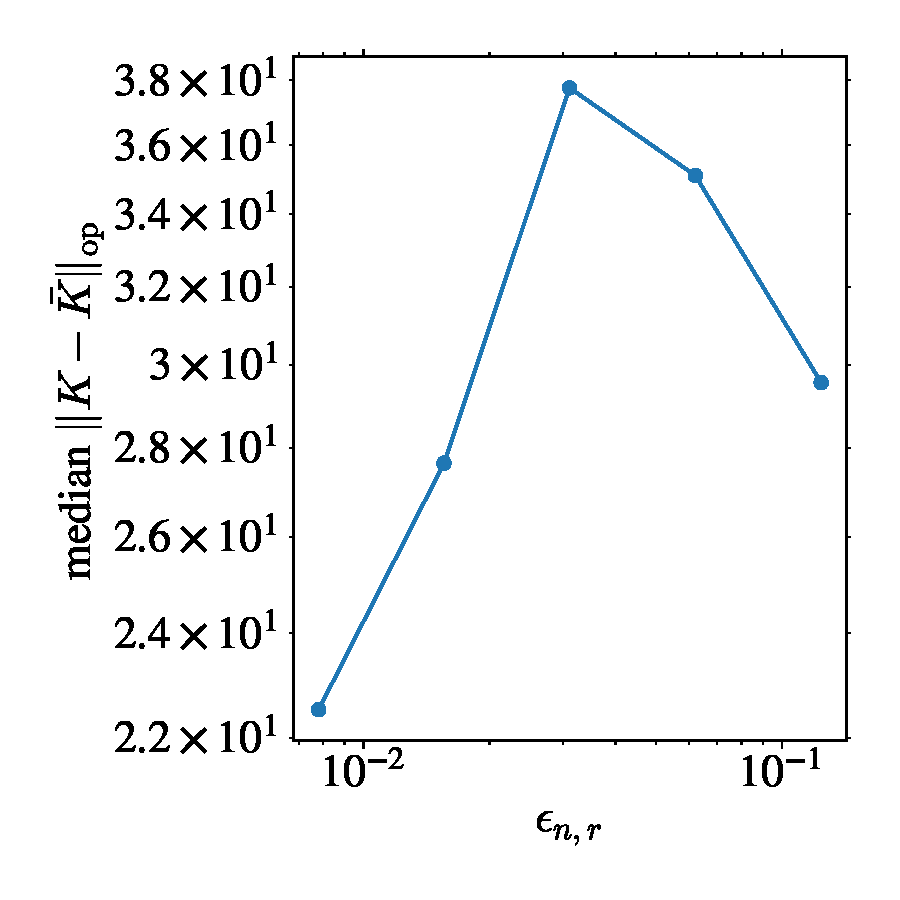
\includegraphics[width=0.92\linewidth]{../../data/feynman/true_finite_ntk_outputs_clean/true_finite_ntk_rank_defect_scaling.pdf}
\end{minipage}
\vspace{-0.5em}
\caption{True finite-network NTK checks computed by autodiff. Left: empirical operator deviations follow the predicted normalization. Right: the low-rank excess deviation tracks the rank-defect scale; at the full-rank endpoint the rank-defect contribution disappears, while ordinary finite-width and numerical residuals can remain.}
\label{fig:true-ntk-operator-rank}
\end{figure}

\begin{figure}[H]
\centering
\begin{minipage}{0.30\linewidth}
\centering
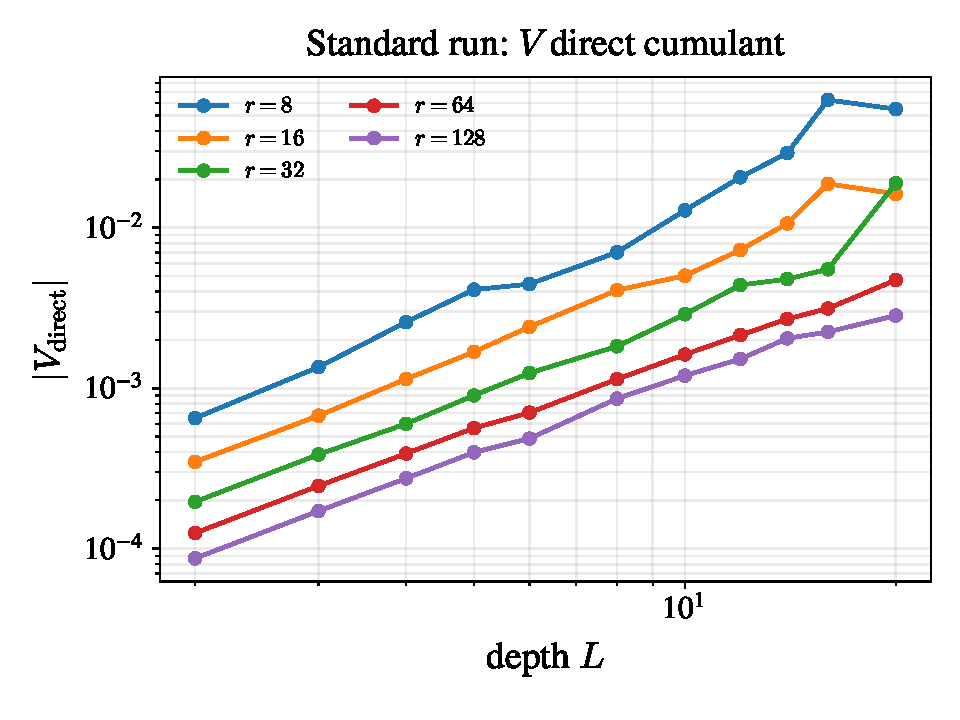
\includegraphics[width=0.92\linewidth]{../../data/feynman/true_finite_ntk_cumulants_very_long/cumulant_loglog_V_same_off.pdf}
\end{minipage}
\hfill
\begin{minipage}{0.30\linewidth}
\centering
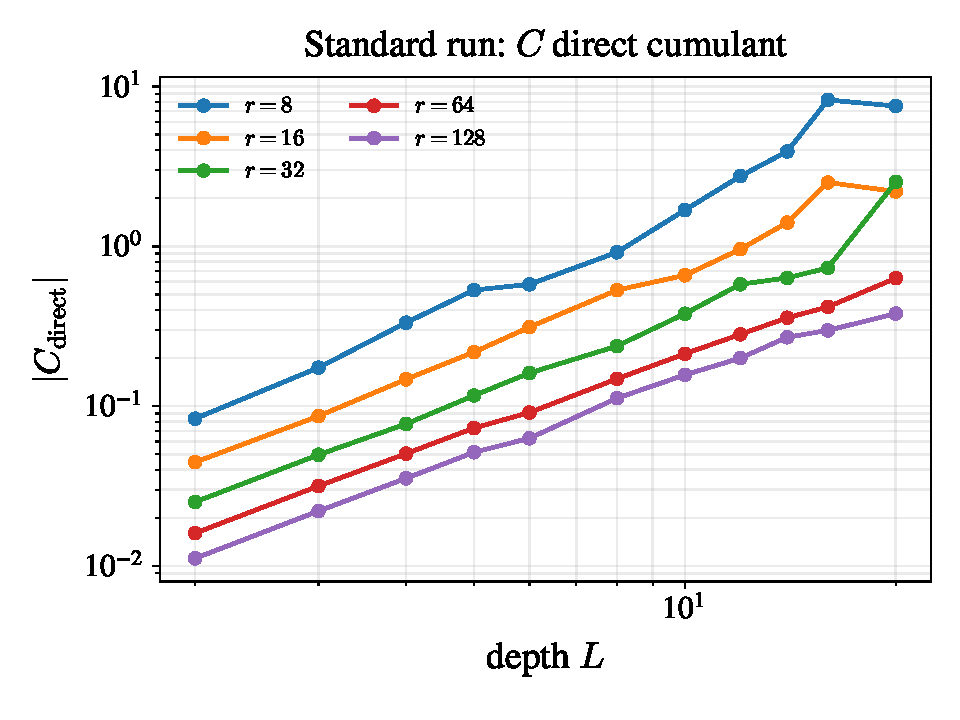
\includegraphics[width=0.92\linewidth]{../../data/feynman/true_finite_ntk_cumulants_very_long/cumulant_loglog_C_same_off.pdf}
\end{minipage}
\hfill
\begin{minipage}{0.30\linewidth}
\centering
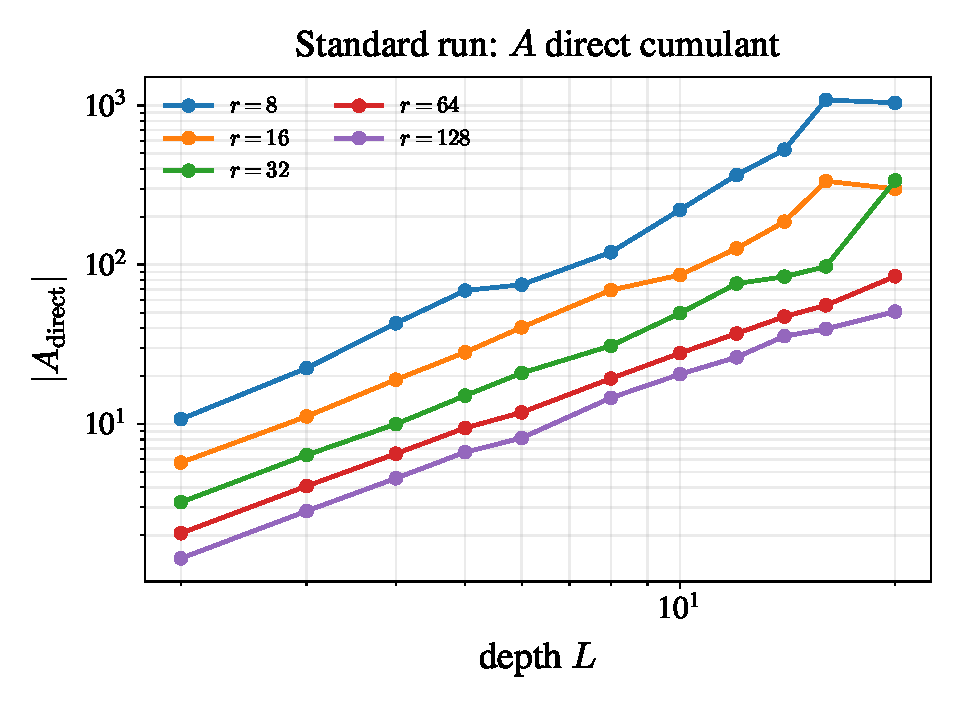
\includegraphics[width=0.92\linewidth]{../../data/feynman/true_finite_ntk_cumulants_very_long/cumulant_loglog_A_same_off.pdf}
\end{minipage}
\vspace{0.4em}
\begin{minipage}{0.30\linewidth}
\centering
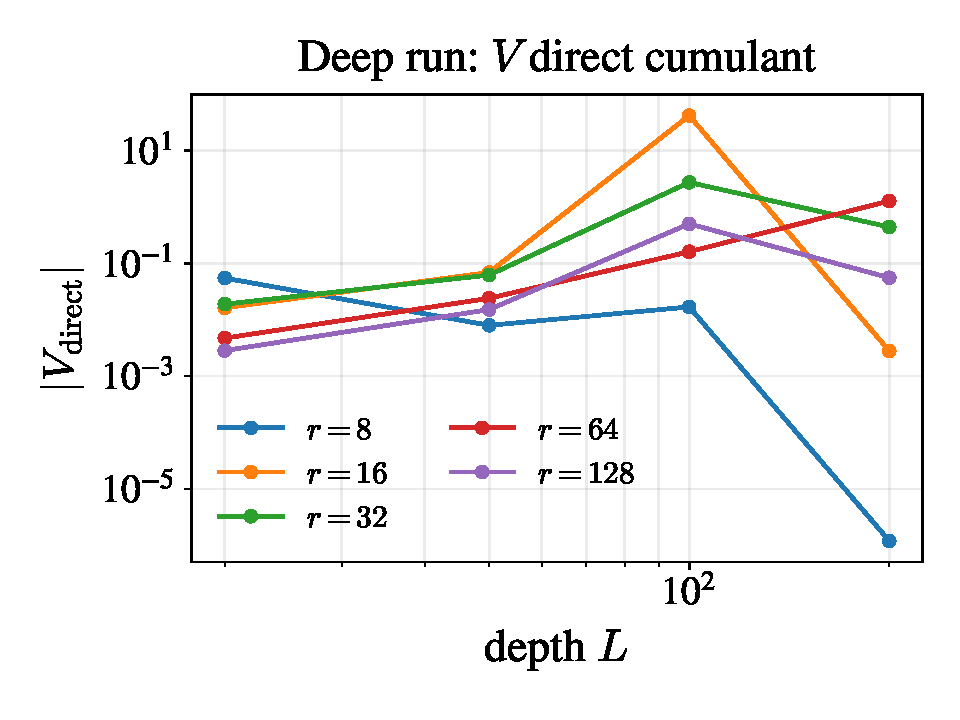
\includegraphics[width=0.92\linewidth]{../../data/feynman/true_finite_ntk_cumulants_depth_20_50_100_200/cumulant_loglog_V_same_off.pdf}
\end{minipage}
\hfill
\begin{minipage}{0.30\linewidth}
\centering
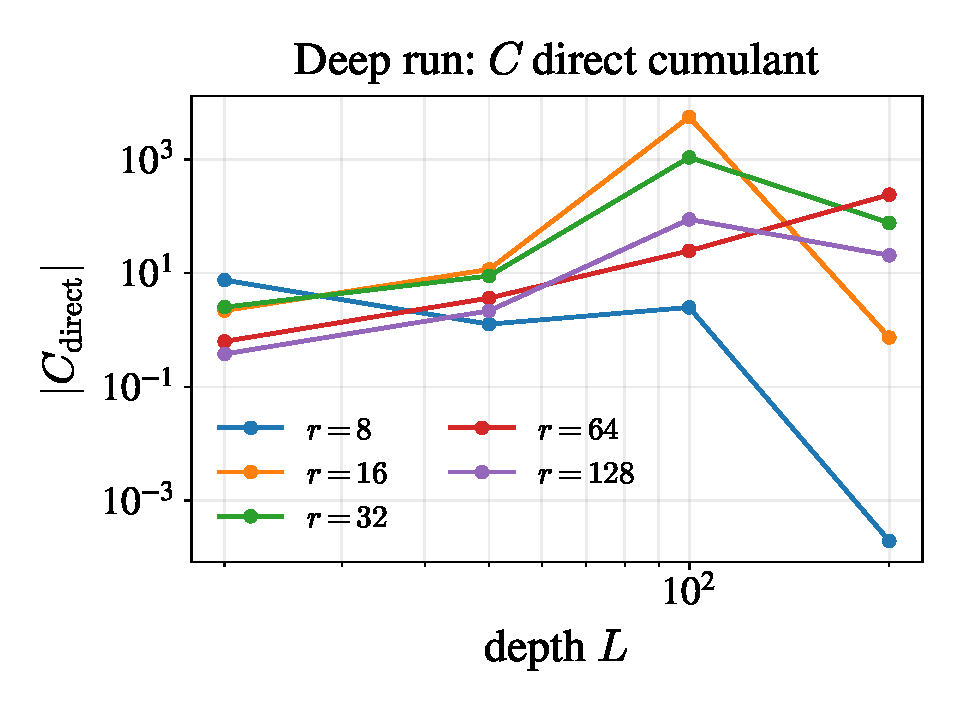
\includegraphics[width=0.92\linewidth]{../../data/feynman/true_finite_ntk_cumulants_depth_20_50_100_200/cumulant_loglog_C_same_off.pdf}
\end{minipage}
\hfill
\begin{minipage}{0.30\linewidth}
\centering
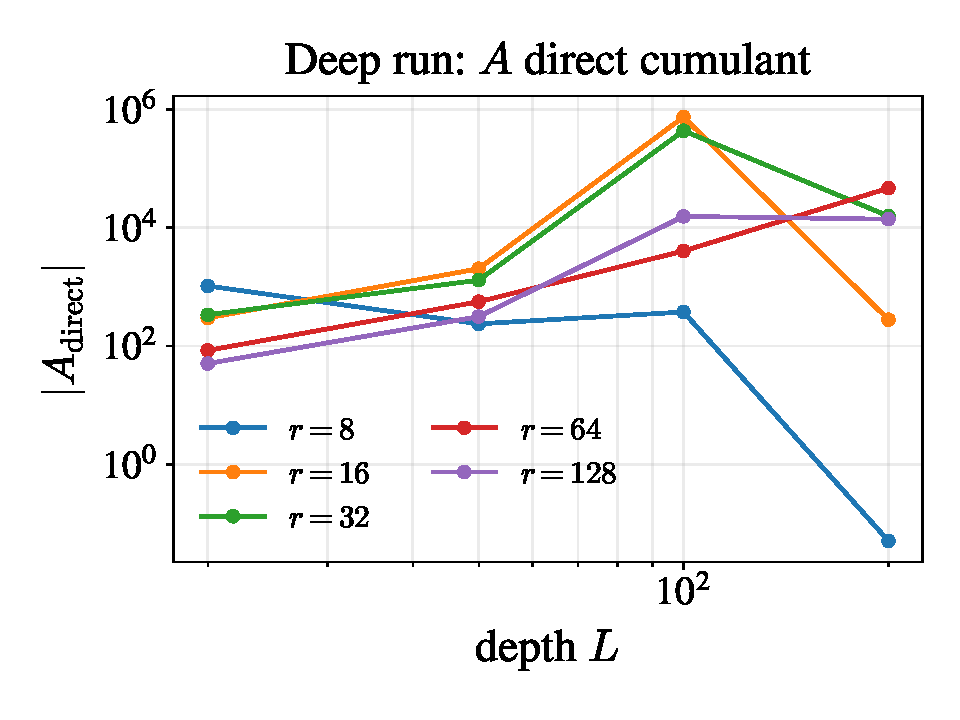
\includegraphics[width=0.92\linewidth]{../../data/feynman/true_finite_ntk_cumulants_depth_20_50_100_200/cumulant_loglog_A_same_off.pdf}
\end{minipage}
\vspace{-0.5em}
\caption{Log-log finite-network cumulant magnitudes. Top: the standard long run. Bottom: the \(L\in\{20,50,100,200\}\) deep stress test. These plots show effective depth slopes directly, before normalizing by the proposed \(L\), \(L^2\), and \(L^3\) scales.}
\label{fig:appendix-cumulant-loglog}
\end{figure}

\begin{table}[H]
\centering
\caption{Exact full-rank matching for true empirical NTKs at \(n=r=128\), \(m=8\), \(d=16\). Differences remain at numerical precision up to depth \(L=200\), confirming Theorem \ref{thm:pathwise}.}
\label{tab:full-rank-matching}
\begin{tabular}{ccc}
\toprule
Depth & max absolute NTK difference & relative difference \\
\midrule
2 & \(8.88\cdot10^{-16}\) & \(8.09\cdot10^{-17}\) \\
4 & \(3.55\cdot10^{-15}\) & \(1.31\cdot10^{-16}\) \\
6 & \(5.33\cdot10^{-15}\) & \(4.05\cdot10^{-16}\) \\
8 & \(3.55\cdot10^{-15}\) & \(4.20\cdot10^{-16}\) \\
10 & \(6.22\cdot10^{-15}\) & \(1.14\cdot10^{-15}\) \\
20 & \(1.95\cdot10^{-14}\) & \(3.77\cdot10^{-15}\) \\
50 & \(5.68\cdot10^{-14}\) & \(6.68\cdot10^{-16}\) \\
100 & \(2.14\cdot10^{-15}\) & \(2.35\cdot10^{-14}\) \\
200 & \(8.08\cdot10^{-14}\) & \(1.27\cdot10^{-14}\) \\
\bottomrule
\end{tabular}
\end{table}

\section{MNIST Parameter-Efficiency Snapshot}
\label{app:mnist-details}
This auxiliary experiment is included only as empirical motivation for the rank bottleneck question; it is not used in the NTK proofs. The numerical summary is reported in Table \ref{tab:intro-mnist-lowrank}. MNIST images are flattened to \(784\) dimensions and normalized with the standard MNIST mean and variance. All models are trained with cross-entropy using Adam with learning rate \(10^{-3}\), batch size \(128\), \(30\) epochs, seed \(42\), and gradient clipping at norm \(1\). The dense baseline is a ReLU MLP with hidden width \(512\) and two hidden layers. The low-rank models use the same width and a rank bottleneck; in the small-rank rows, one random feature side of the bottleneck is held fixed and the low-rank trainable maps and classifier are optimized.

\section{Why Strict Positive NMF Is Not Covered}
This appendix explains why signed isometric low rank is not the same mathematical model as nonnegative matrix factorization.
The model in \eqref{eq:intro-model} is signed and isometric. The right factor \(B\) is unconstrained and the frozen left factor \(U\) has orthonormal columns. Strict nonnegative matrix factorization imposes a cone constraint and changes the tangent space even at initialization. Its NTK is a projected or conic kernel, not the fixed linear-subspace kernel analyzed here. Therefore the results should not be cited as a theorem for positive NMF without a separate analysis of active constraints, boundary faces, and cone-projected gradients.

\section{Proof Details for Endpoint Constants}
\label{app:proof-endpoint-constants}
This appendix gives the elementary ReLU moment calculation that produces the endpoint constants used in the main text. For \(g\sim\mathcal N(0,1)\), let
\[
X_0=2(g_+)^2,
\qquad
Y_0=2\one_{\{g>0\}}.
\]

\begin{figure}[H]
\centering
\resizebox{\linewidth}{!}{%
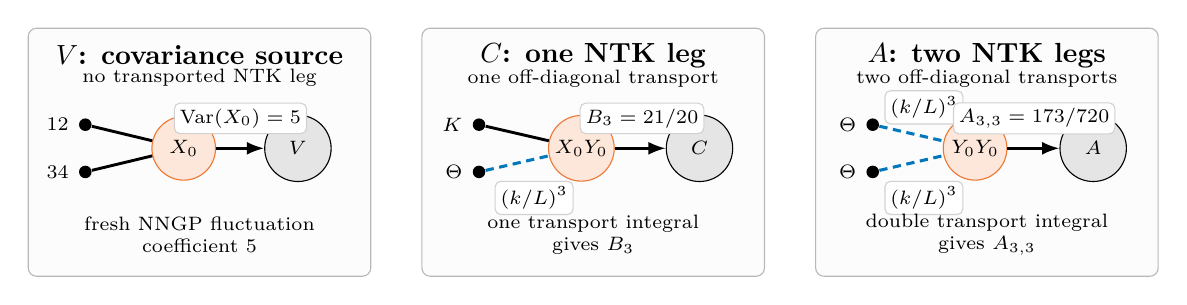
\begin{tikzpicture}[
  x=1cm,
  y=1cm,
  panel/.style={draw=black!28, rounded corners=3pt, fill=black!1, minimum width=4.35cm, minimum height=3.15cm},
  ext/.style={circle, fill=black, inner sep=1.6pt},
  nngp/.style={line width=1.05pt},
  ntk/.style={color=color1, dash pattern=on 3pt off 2pt, line width=1.1pt},
  src/.style={circle, draw=color2, fill=color2!18, minimum size=23pt, inner sep=1.5pt},
  tensor/.style={circle, draw=black, fill=black!10, minimum size=24pt, inner sep=1.5pt},
  flow/.style={-{Latex[length=2.2mm]}, line width=0.9pt},
  tag/.style={draw=black!18, rounded corners=2pt, fill=white, inner sep=2pt, font=\scriptsize},
  every node/.style={font=\small}
]
\node[panel] at (0,0) {};
\node[font=\bfseries] at (0,1.23) {\(V\): covariance source};
\node[font=\scriptsize, align=center] at (0,0.94) {no transported NTK leg};
\node[ext,label=left:{\scriptsize \(12\)}] (v1) at (-1.45,0.35) {};
\node[ext,label=left:{\scriptsize \(34\)}] (v2) at (-1.45,-0.25) {};
\node[src] (vs) at (-0.2,0.05) {\scriptsize \(X_0\)};
\node[tensor] (vt) at (1.25,0.05) {\scriptsize \(V\)};
\draw[nngp] (v1) -- (vs);
\draw[nngp] (v2) -- (vs);
\draw[flow] (vs) -- (vt);
\node[tag] at (0.52,0.43) {\(\Var(X_0)=5\)};
\node[font=\scriptsize, align=center] at (0,-1.05) {fresh NNGP fluctuation\\coefficient \(5\)};

\node[panel] at (5.0,0) {};
\node[font=\bfseries] at (5.0,1.23) {\(C\): one NTK leg};
\node[font=\scriptsize, align=center] at (5.0,0.94) {one off-diagonal transport};
\node[ext,label=left:{\scriptsize \(K\)}] (c1) at (3.55,0.35) {};
\node[ext,label=left:{\scriptsize \(\Theta\)}] (c2) at (3.55,-0.25) {};
\node[src] (cs) at (4.85,0.05) {\scriptsize \(X_0Y_0\)};
\node[tensor] (ct) at (6.35,0.05) {\scriptsize \(C\)};
\draw[nngp] (c1) -- (cs);
\draw[ntk] (c2) -- (cs);
\draw[flow] (cs) -- (ct);
\node[tag] at (4.25,-0.58) {\((k/L)^3\)};
\node[tag] at (5.62,0.43) {\(B_3=21/20\)};
\node[font=\scriptsize, align=center] at (5.0,-1.05) {one transport integral\\gives \(B_3\)};

\node[panel] at (10.0,0) {};
\node[font=\bfseries] at (10.0,1.23) {\(A\): two NTK legs};
\node[font=\scriptsize, align=center] at (10.0,0.94) {two off-diagonal transports};
\node[ext,label=left:{\scriptsize \(\Theta\)}] (a1) at (8.55,0.35) {};
\node[ext,label=left:{\scriptsize \(\Theta\)}] (a2) at (8.55,-0.25) {};
\node[src] (as) at (9.85,0.05) {\scriptsize \(Y_0Y_0\)};
\node[tensor] (at) at (11.35,0.05) {\scriptsize \(A\)};
\draw[ntk] (a1) -- (as);
\draw[ntk] (a2) -- (as);
\draw[flow] (as) -- (at);
\node[tag] at (9.20,0.57) {\((k/L)^3\)};
\node[tag] at (9.20,-0.58) {\((k/L)^3\)};
\node[tag] at (10.60,0.43) {\(A_{3,3}=173/720\)};
\node[font=\scriptsize, align=center] at (10.0,-1.05) {double transport integral\\gives \(A_{3,3}\)};
\end{tikzpicture}
}
\caption{Endpoint diagrams for the constants in \eqref{eq:endpoint-constants}. Each panel separates the local ReLU atom from the external transport: \(V\) has no transported NTK leg, \(C\) has one off-diagonal NTK leg, and \(A\) has two.}
\label{fig:endpoint-constant-diagrams}
\end{figure}

Here \(X_0\) is the scalar ReLU covariance atom and \(Y_0\) is the scalar derivative atom appearing on an NTK leg. Since \(\E[g_+^2]=1/2\) and \(\E[g_+^4]=3/2\),
\[
\E X_0=1,
\qquad
\E X_0^2=6,
\qquad
\Var(X_0)=5.
\]
Also \(\E Y_0=1\), \(\E Y_0^2=2\), and therefore \(\Var(Y_0)=1\). Finally,
\[
\E X_0Y_0=\E\!\left[4(g_+)^2\one_{\{g>0\}}\right]=4\E[g_+^2]=2,
\qquad
\Cov(X_0,Y_0)=2-1=1.
\]
Thus a fresh \(K\)-\(K\) source has endpoint coefficient \(5\).

It remains to explain the transported NTK legs. If a leg born at layer \(k\) is transported to depth \(L\), the ReLU edge-of-chaos off-diagonal derivative satisfies
\[
\prod_{j=k+1}^{L}\dot{\mathcal C}(\rho_j)
=\prod_{j=k+1}^{L}\left(1-\frac3j+O\!\left(\frac{\log j}{j^2}\right)\right)
=\left(\frac{k}{L}\right)^3(1+o(1)).
\]
More generally, write the transport exponent as \(\lambda\). The finite depth sum for one transported NTK leg is a Riemann/Beta-sum limit,
\[
B_\lambda
=\lim_{L\to\infty}\frac1L\sum_{k=1}^{L}
\left(\frac{k}{L}\right)^\lambda
\left(1+4\frac{k}{L}\right)
=\frac{1}{\lambda+1}+\frac{4}{\lambda+2}
=\frac1{\lambda+1}\left(5-\frac4{\lambda+2}\right).
\]
The two-leg calculation is the same pairing-basis projection with two transported legs. Its endpoint sum is
\[
A_{\lambda,\mu}
=\frac{1}{(\lambda+1)(\mu+1)}
\left(5-\frac4{\lambda+2}-\frac4{\mu+2}
+\frac4{\lambda+\mu+3}\right).
\]
Consequently, for the isolated off-diagonal ReLU modes used in the main text, \(\lambda=\mu=3\), and
\[
V=5,
\qquad
C=B_3=\frac{21}{20},
\qquad
A=A_{3,3}=\frac{173}{720}.
\]

\end{document}
